\section{Data and Monte Carlo simulations samples}
%\begin{tcolorbox}[breakable,colback=black!5!white,colframe=red!80!black,width=\textwidth]
%\chapter*{Data and Monte Carlo samples}
%\end{tcolorbox}
\label{chap:samples}

\subsection{Signal samples}

Signal samples of a spin-2 (Bulk Graviton) decaying in a pair of \Z bosons are exploited in the analysis. To target the final state, one of the two \Z bosons is forced to decay into neutrinos, while the other \Z is forced to decay hadronically. The signal samples are produced in the narrow-width approximation by setting the resonance with to 0.1\% of its mass. Twelve mass points with 100000 events each are simulated, with a $m_{\G}$ ranging from 600 \GeV up to 4500 \GeV.

\noindent Additionally, samples of a spin-1 HVT-like \Wp resonance decaying in a \Z boson and a \W boson are studied. The \Z boson is forced to decay into neutrinos, and the \W boson is forced to decay hadronically. Also in this case the signal samples are produced in the narrow-width approximation by setting the resonance with to 0.1\% of its mass. Twelve mass points with 100000 events each are simulated, with a $m_{\Wp}$ ranging from 600 \GeV up to 4500 \GeV.

\noindent The signal samples are generated at leading-order (LO) with the {\sc MadGraph5\_aMCatNLO v 2.2.2}~\cite{bib:MADGRAPH} matrix element generator, while hadronization and fragmentation are handled by \PYTHIA 8~\cite{bib:PYTHIA} version 8.2121 with CUETP8M1~\cite{bib:CUETP8M1} tuning. A full detector simulation and event reconstruction has been performed with \GEANTfour~\cite{bib:GEANT4} and CMSSW. The detector alignement scenario, calibrations and pile-up distributions are generated according to the expectations in 2016 data.
%All signal samples belong to the {\tt RunIISummer16MiniAODv2\_PUMoriond17-80X\_mcRun2} campaign.

\noindent All the signal samples used in the analysis and the related properties are reported in Tables~\ref{tab:signal_samples}-\ref{tab:signal_samples_W}.
%Missing W'
%and ~\ref{tab:signal_samples_W}. 
 
 \begin{table}[!htb]
   \begin{center}
   \begin{tabular}{lccc}
 Signal process &  $m_{\G}$ & Events & $\sigma\times\mathcal{B}$ (\pb) \\
 \hline 
\BGinv & 600 GeV & 100000 & 0.27964\\
\BGinv & 800 GeV  & 100000 & 0.27964\\
\BGinv & 1000 GeV  & 100000 & 0.27964\\
\BGinv & 1200 GeV  & 100000 & 0.27964\\
\BGinv & 1400 GeV  & 100000 & 0.27964\\
\BGinv & 1800 GeV  & 100000 & 0.27964\\
\BGinv & 2000 GeV  & 100000 & 0.27964\\
\BGinv & 2500 GeV  & 100000 & 0.27964\\
\BGinv & 3000 GeV  & 100000 & 0.27964\\
\BGinv & 3500 GeV  & 100000 & 0.27964\\
\BGinv & 4000 GeV  & 100000 & 0.27964\\
\BGinv & 4500 GeV  & 100000 & 0.27964\\
   \end{tabular}
   \end{center}
   \caption{Spin-2 (Bulk Graviton) signal samples and production cross sections (assumed to be $1\pb$) multiplied by the respective branching fractions of the \Z decays considered ($\mathcal{B}(\Z \to \nu\nu) = 0.20$, $\mathcal{B}(\Z \to qq) = 0.6991$). \label{tab:signal_samples}}
 \end{table}

 \begin{table}[!htb]
   \begin{center}
   \begin{tabular}{lccc}
 Signal process &  $m_{\Wp}$ & Events & $\sigma\times\mathcal{B}$ (\pb) \\
 \hline
\Wpinv & 600 GeV & 100000 & 0.13482\\
\Wpinv & 800 GeV  & 100000 & 0.13482\\
\Wpinv & 1000 GeV  & 100000 & 0.13482\\
\Wpinv & 1200 GeV  & 100000 & 0.13482\\
\Wpinv & 1400 GeV  & 100000 & 0.13482\\
\Wpinv & 1800 GeV  & 100000 & 0.13482\\
\Wpinv & 2000 GeV  & 100000 & 0.13482\\
\Wpinv & 2500 GeV  & 100000 & 0.13482\\
\Wpinv & 3000 GeV  & 100000 & 0.13482\\
\Wpinv & 3500 GeV  & 100000 & 0.13482\\
\Wpinv & 4000 GeV  & 100000 & 0.13482\\
\Wpinv & 4500 GeV  & 100000 & 0.13482\\
   \end{tabular}
   \end{center}
   \caption{Spin-1 (W') signal samples and production cross sections (assumed to be $1\pb$) multiplied by the \Z and \W branching fraction ($\mathcal{B}(\Z \to \nu\nu) = 0.2$, $\mathcal{B}(\W \to qq) = 0.6760$).\label{tab:signal_samples_W}}
 \end{table}


\subsection{Signal characterization}

This analysis is performed in a high mass region (from 1~\TeV to 4.5~\TeV). The \MADGRAPH algorithm generates the hard process production in the collision with \pt = 0. In the next step of the simulation, during the hadronization, \PYTHIA adds the QCD ISR (initial state radiation) and consequently a resonance \pt different from 0.
%The transverse mass and \pt distributions of the heavy resonance after the \PYTHIA simulation are shown in fig.~\ref{fig:genSignal1} for Bulk Graviton signal samples (and in fig.~\ref{fig:genSignal2} for \Wp signal samples). The typical \pt is small compared to the mass of the resonance, and about two thirds of the events have \pt smaller than 50 \GeV. The \pt distributions of the electroweak bosons, along with the mass of the hadronically decaying \Z (\W) and the angular separation of the two electroweak bosons in the transverse plane are shown as well.
Kinematical distributions at generator level are showed in fig.~\ref{fig:genGravSignal1}-\ref{fig:genGravSignal3} for spin-2 Bulk Graviton signal, and in fig.~\ref{fig:genWprimeSignal1}-\ref{fig:genWprimeSignal3} for spin-1 HVT \Wp signal.

 \begin{figure}[!htb]
   \begin{center}
     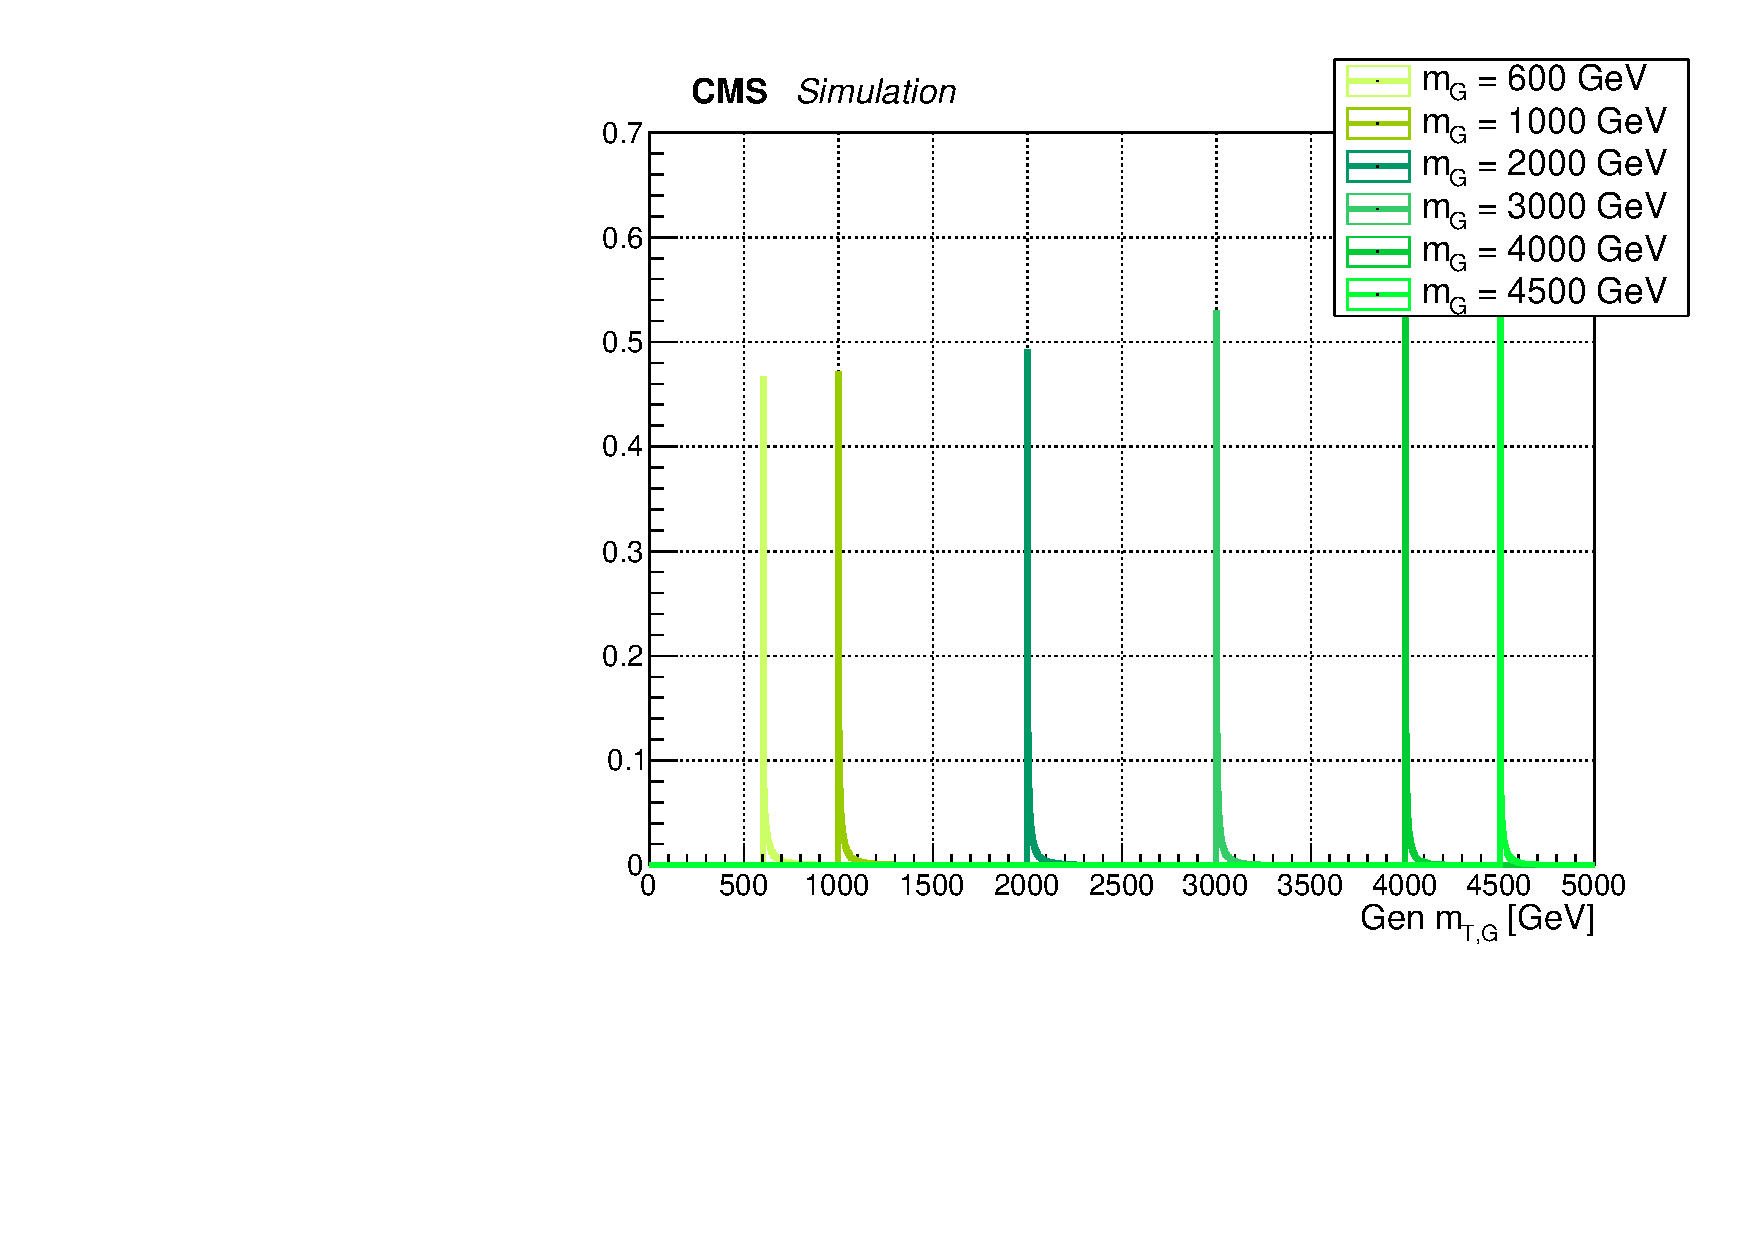
\includegraphics[width=.495\textwidth]{Gen_v9/XZZInv_g_XMT.pdf}%GenPhi1pt.pdf}
     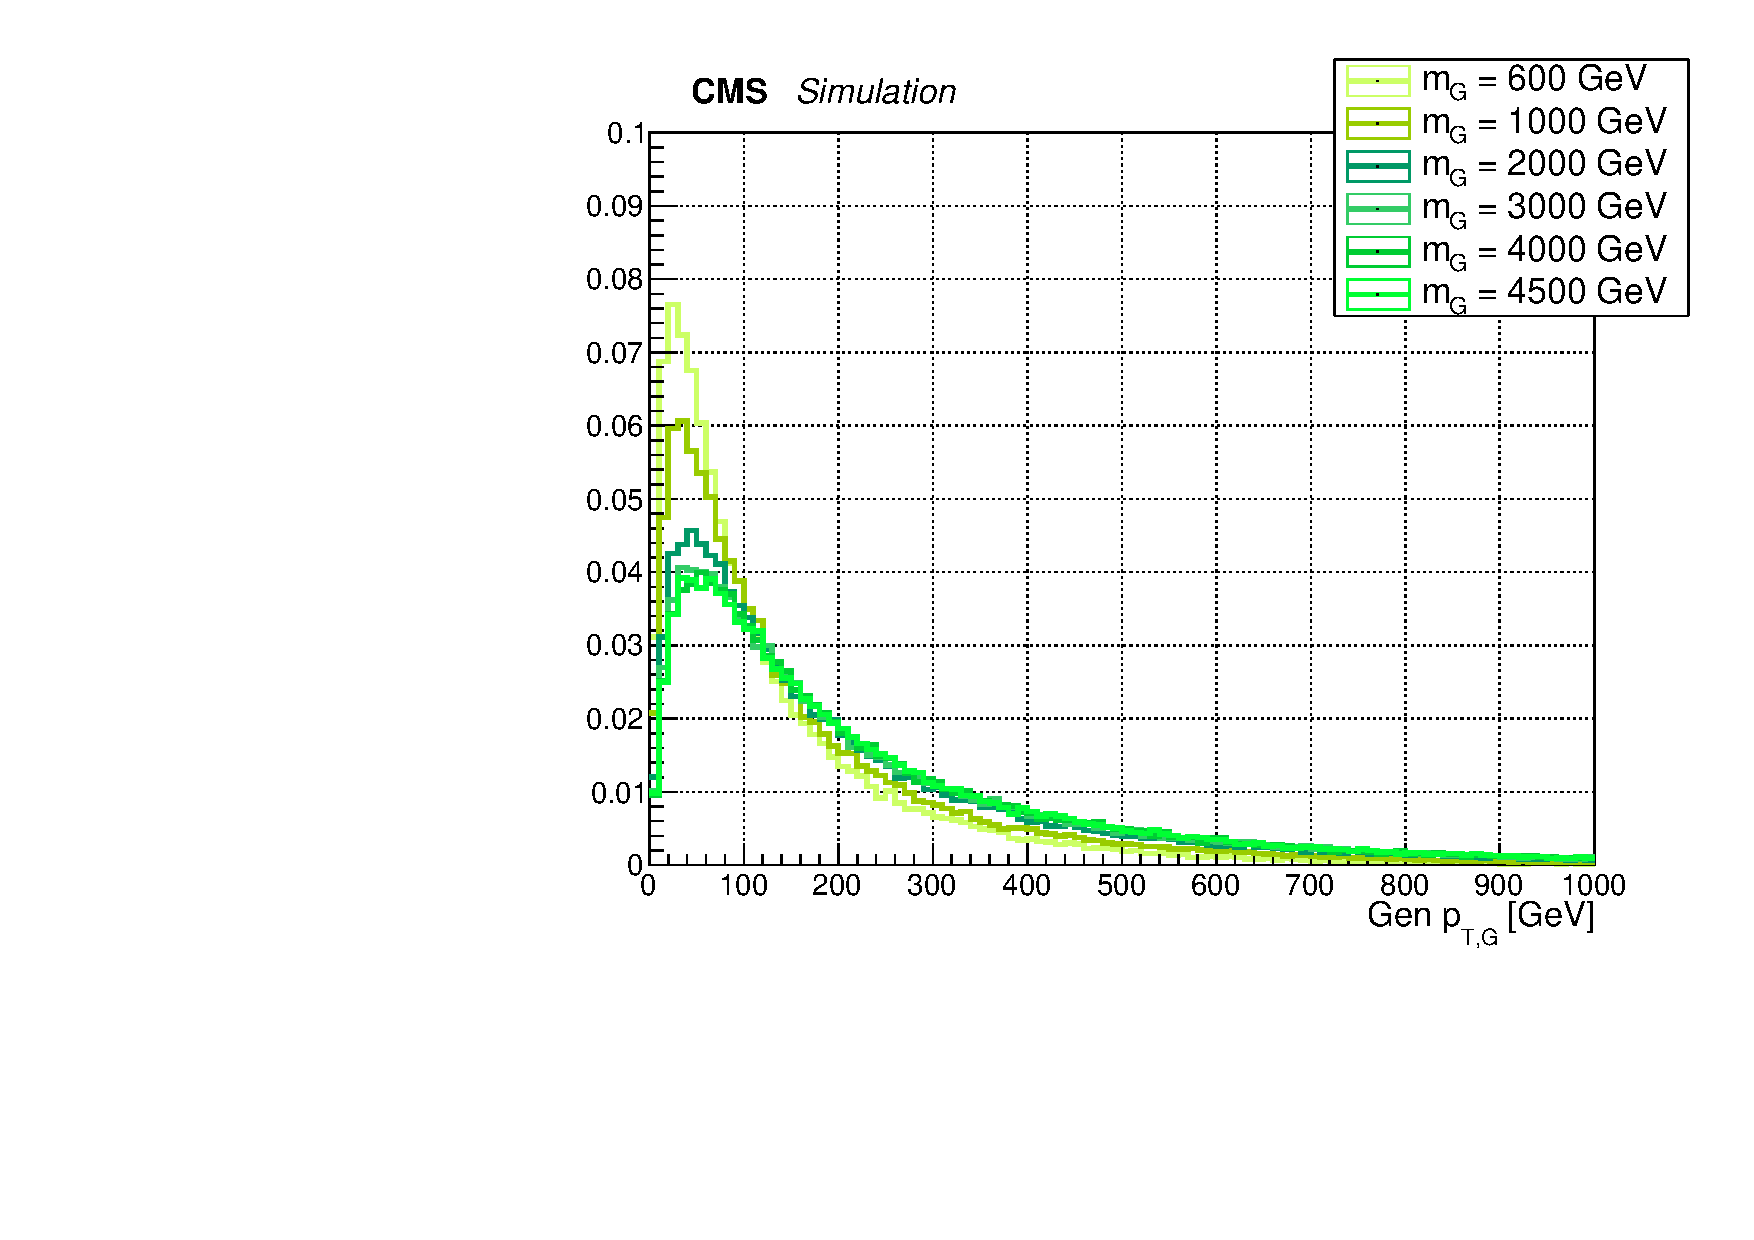
\includegraphics[width=.495\textwidth]{Gen_v9/XZZInv_g_XPt.pdf}%GenPhi1y.pdf}
     %\\
     %\includegraphics[width=.495\textwidth]{Gen_v7/g_ZLepMass.pdf}%GenZmass.pdf}
     %\includegraphics[width=.495\textwidth]{Gen_v7/g_ZHadMass.pdf}%GenHmass.pdf}
     \\
     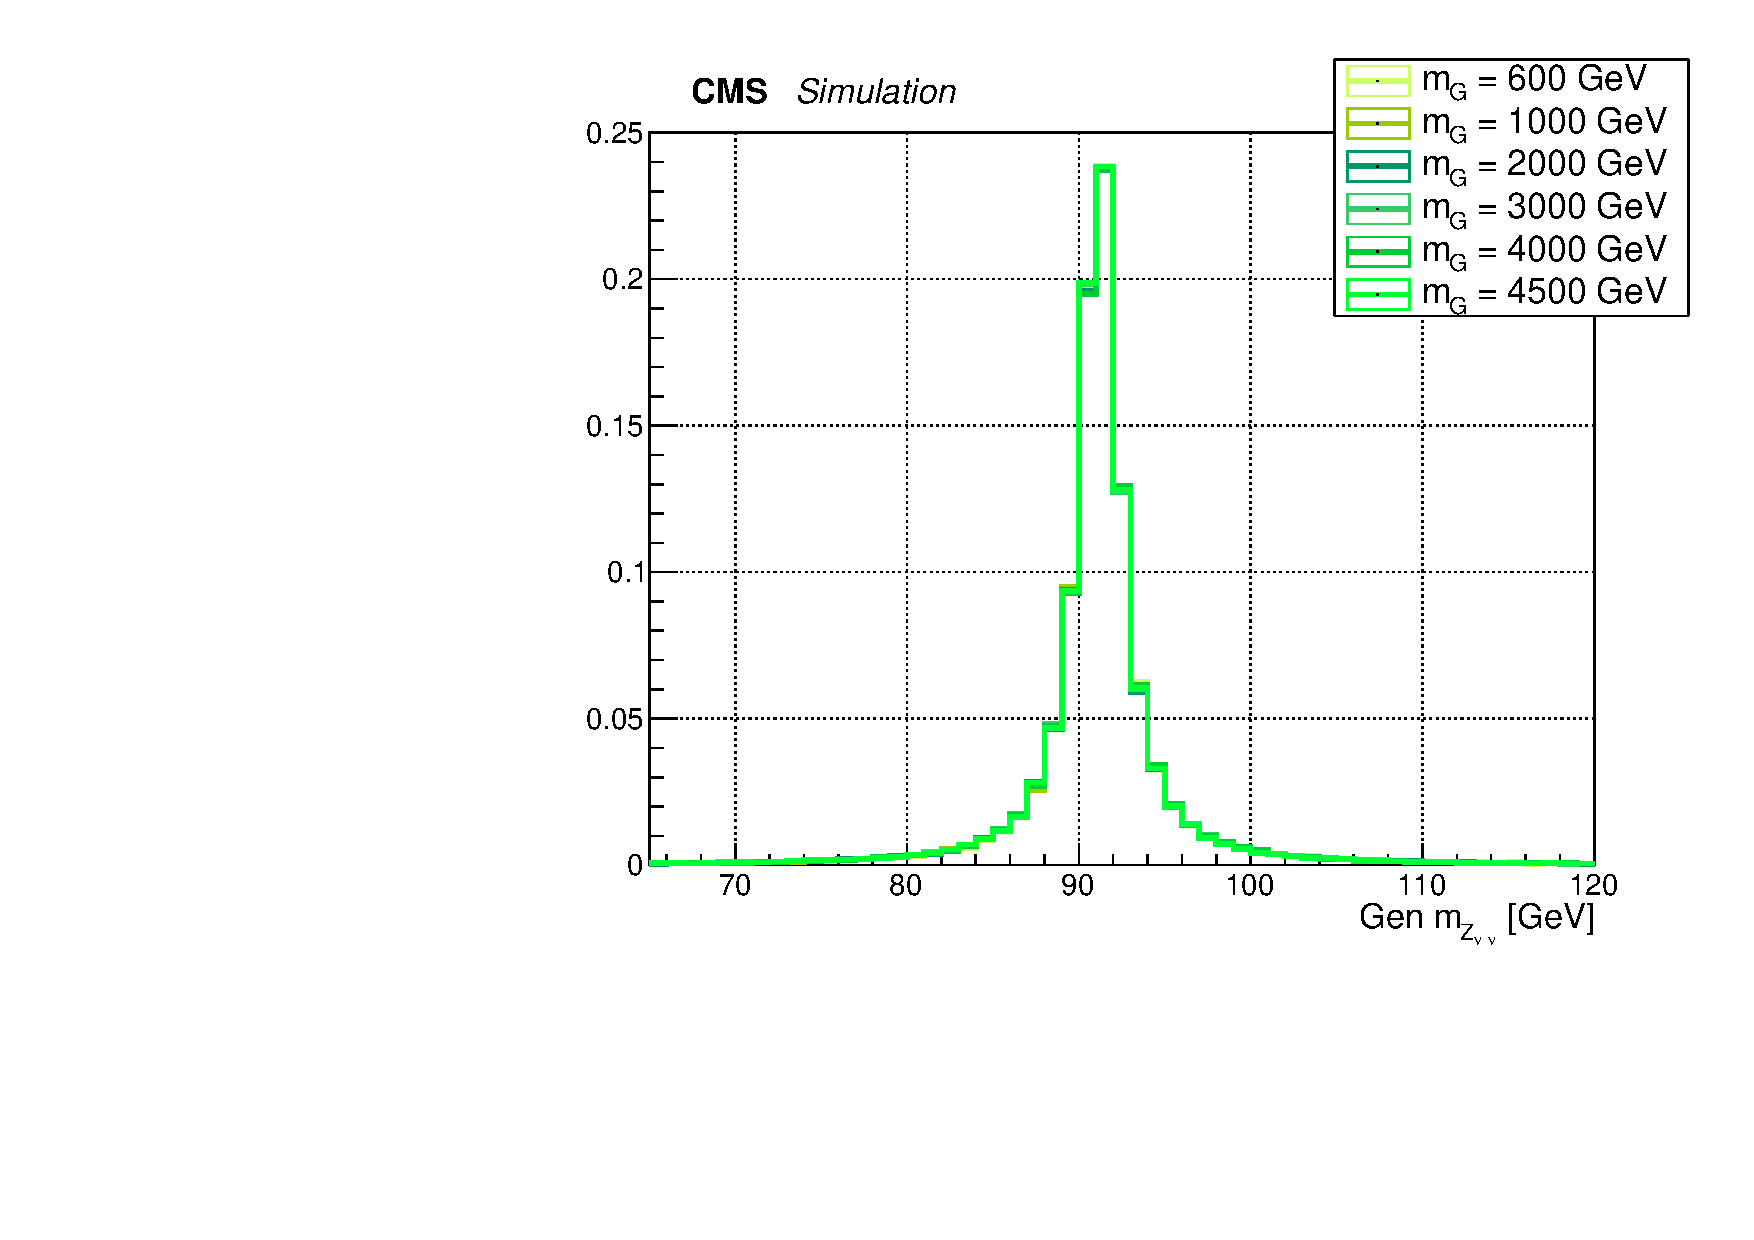
\includegraphics[width=.495\textwidth]{Gen_v9/XZZInv_g_ZLepMass.pdf}%GenZpt.pdf}
     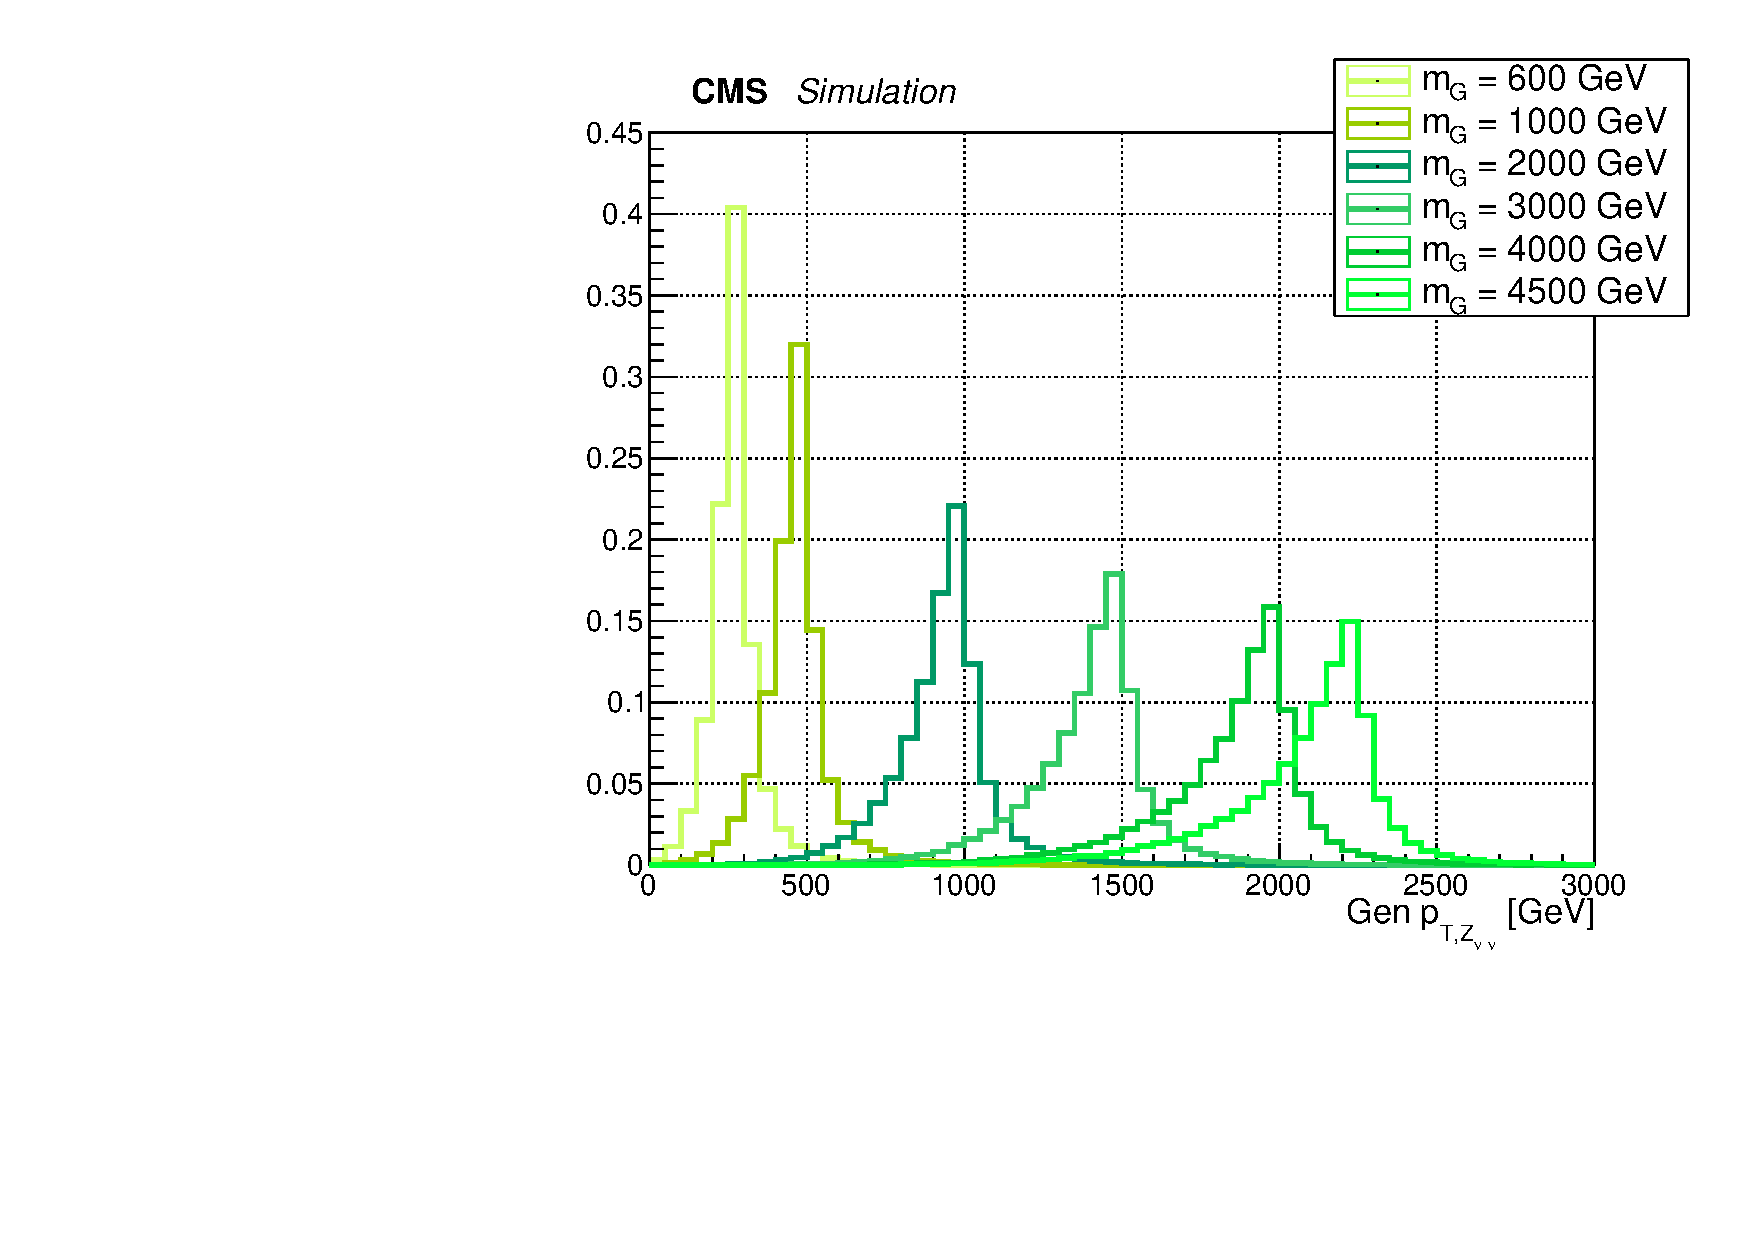
\includegraphics[width=.495\textwidth]{Gen_v9/XZZInv_g_ZLepPt.pdf}%GenHpt.pdf}
     \\
     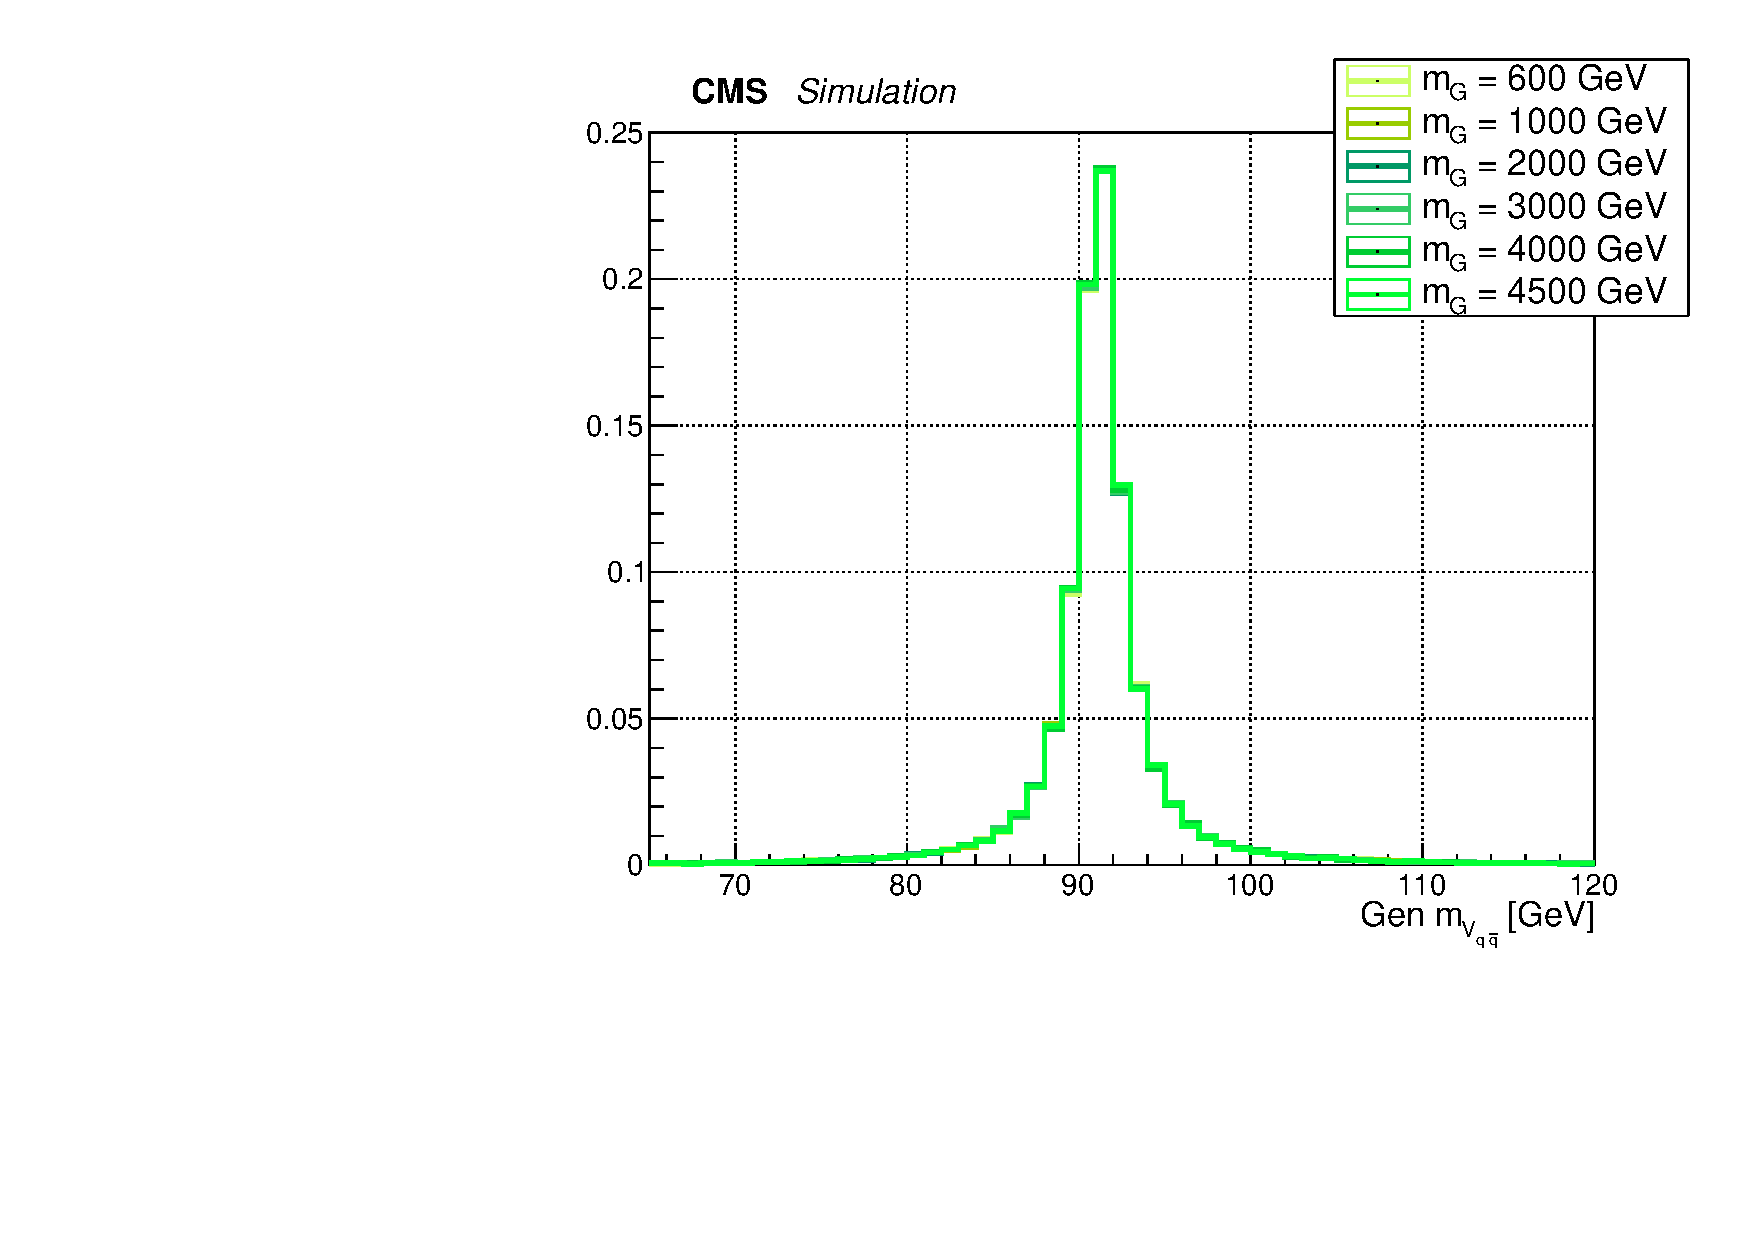
\includegraphics[width=.495\textwidth]{Gen_v9/XZZInv_g_VHadMass.pdf}%GenZdR.pdf}
     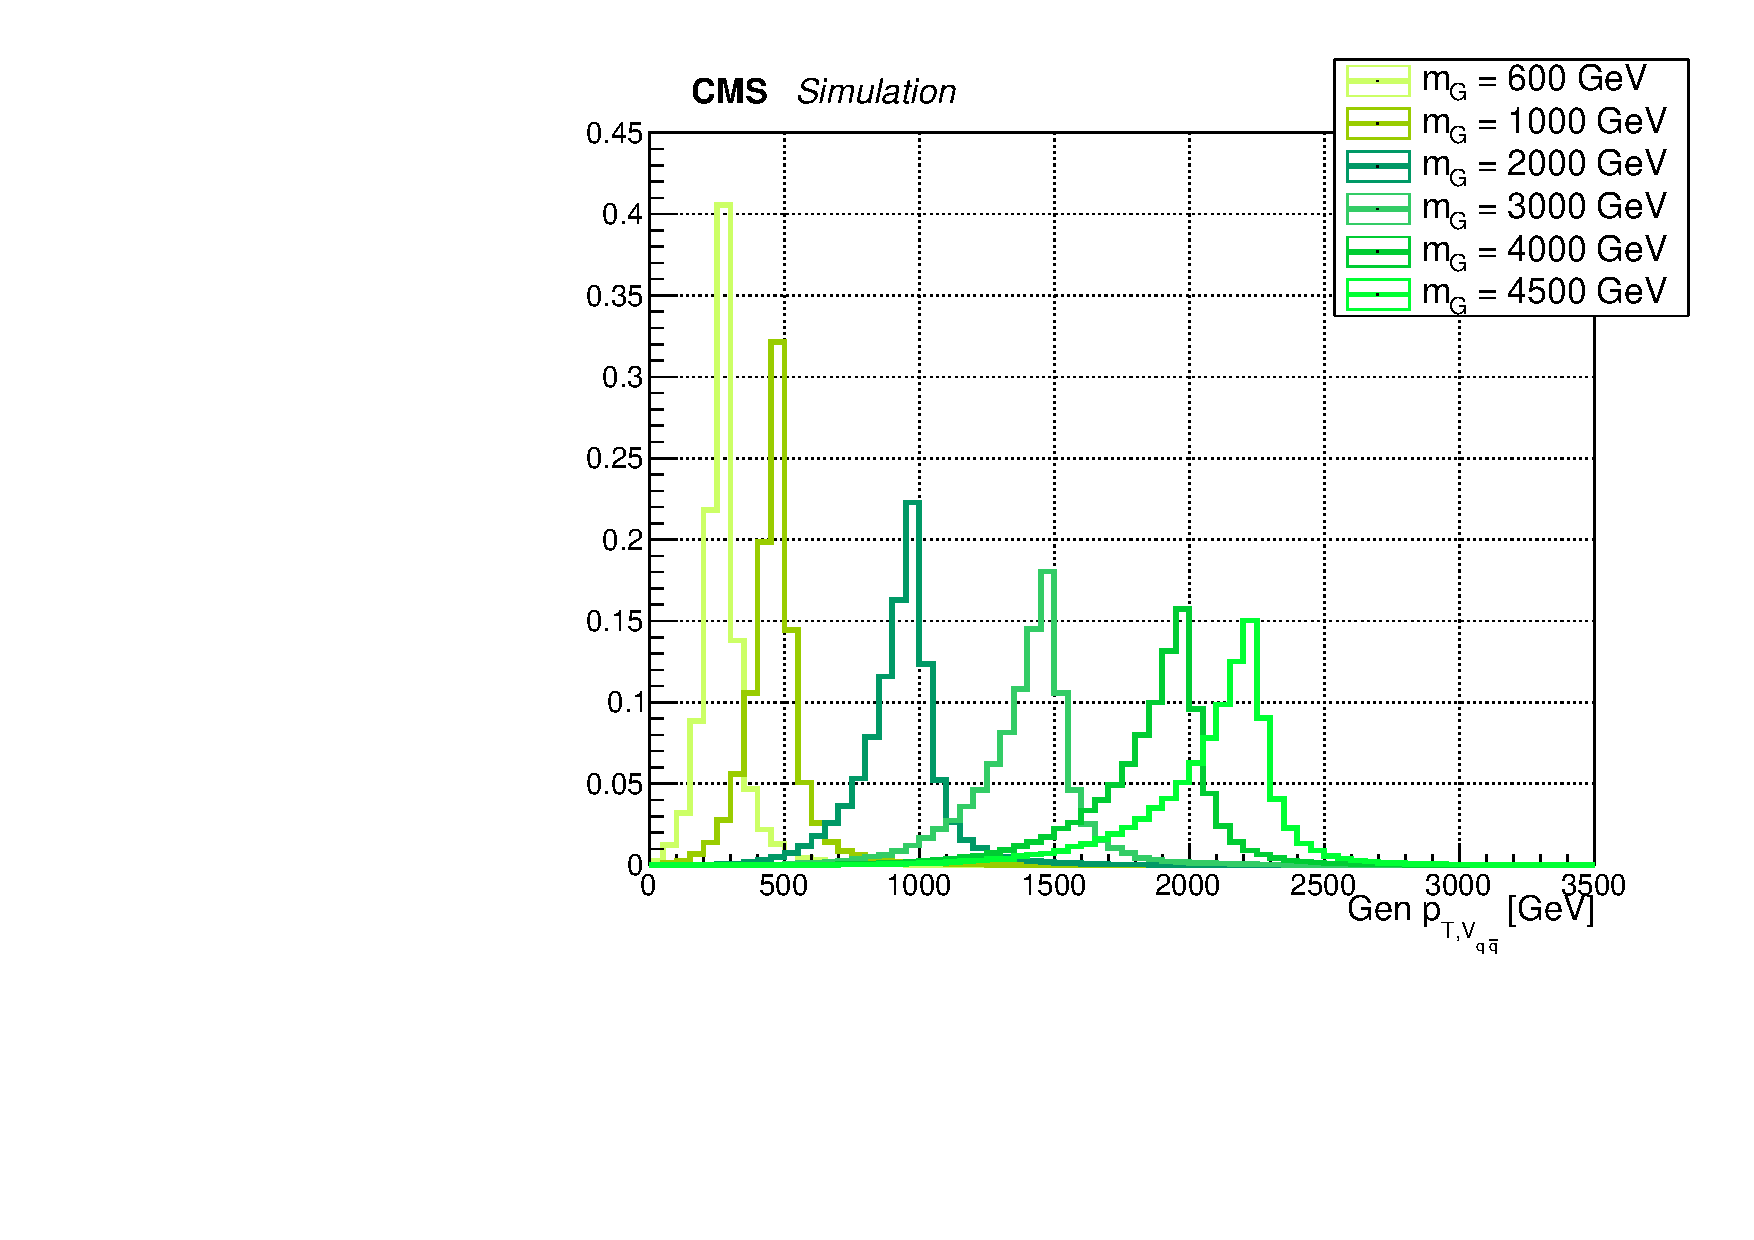
\includegraphics[width=.495\textwidth]{Gen_v9/XZZInv_g_VHadPt.pdf}%GenHdR.pdf}
   \end{center}
   \caption{Main signal kinematic quantities at generation level after parton showering, for spin-2 Bulk Graviton signal, considering different mass hypoteses ($m_{\G} = 0.6, 1, 2, 3, 4, 4.5$ TeV). Top: graviton transverse mass and \pt distributions. Center: invisibly decaying \Z mass and \pt. Bottom: hadronically decaying \Z mass and \pt.}
   \label{fig:genGravSignal1}
 \end{figure}

 \begin{figure}[!htb]
   \begin{center}
     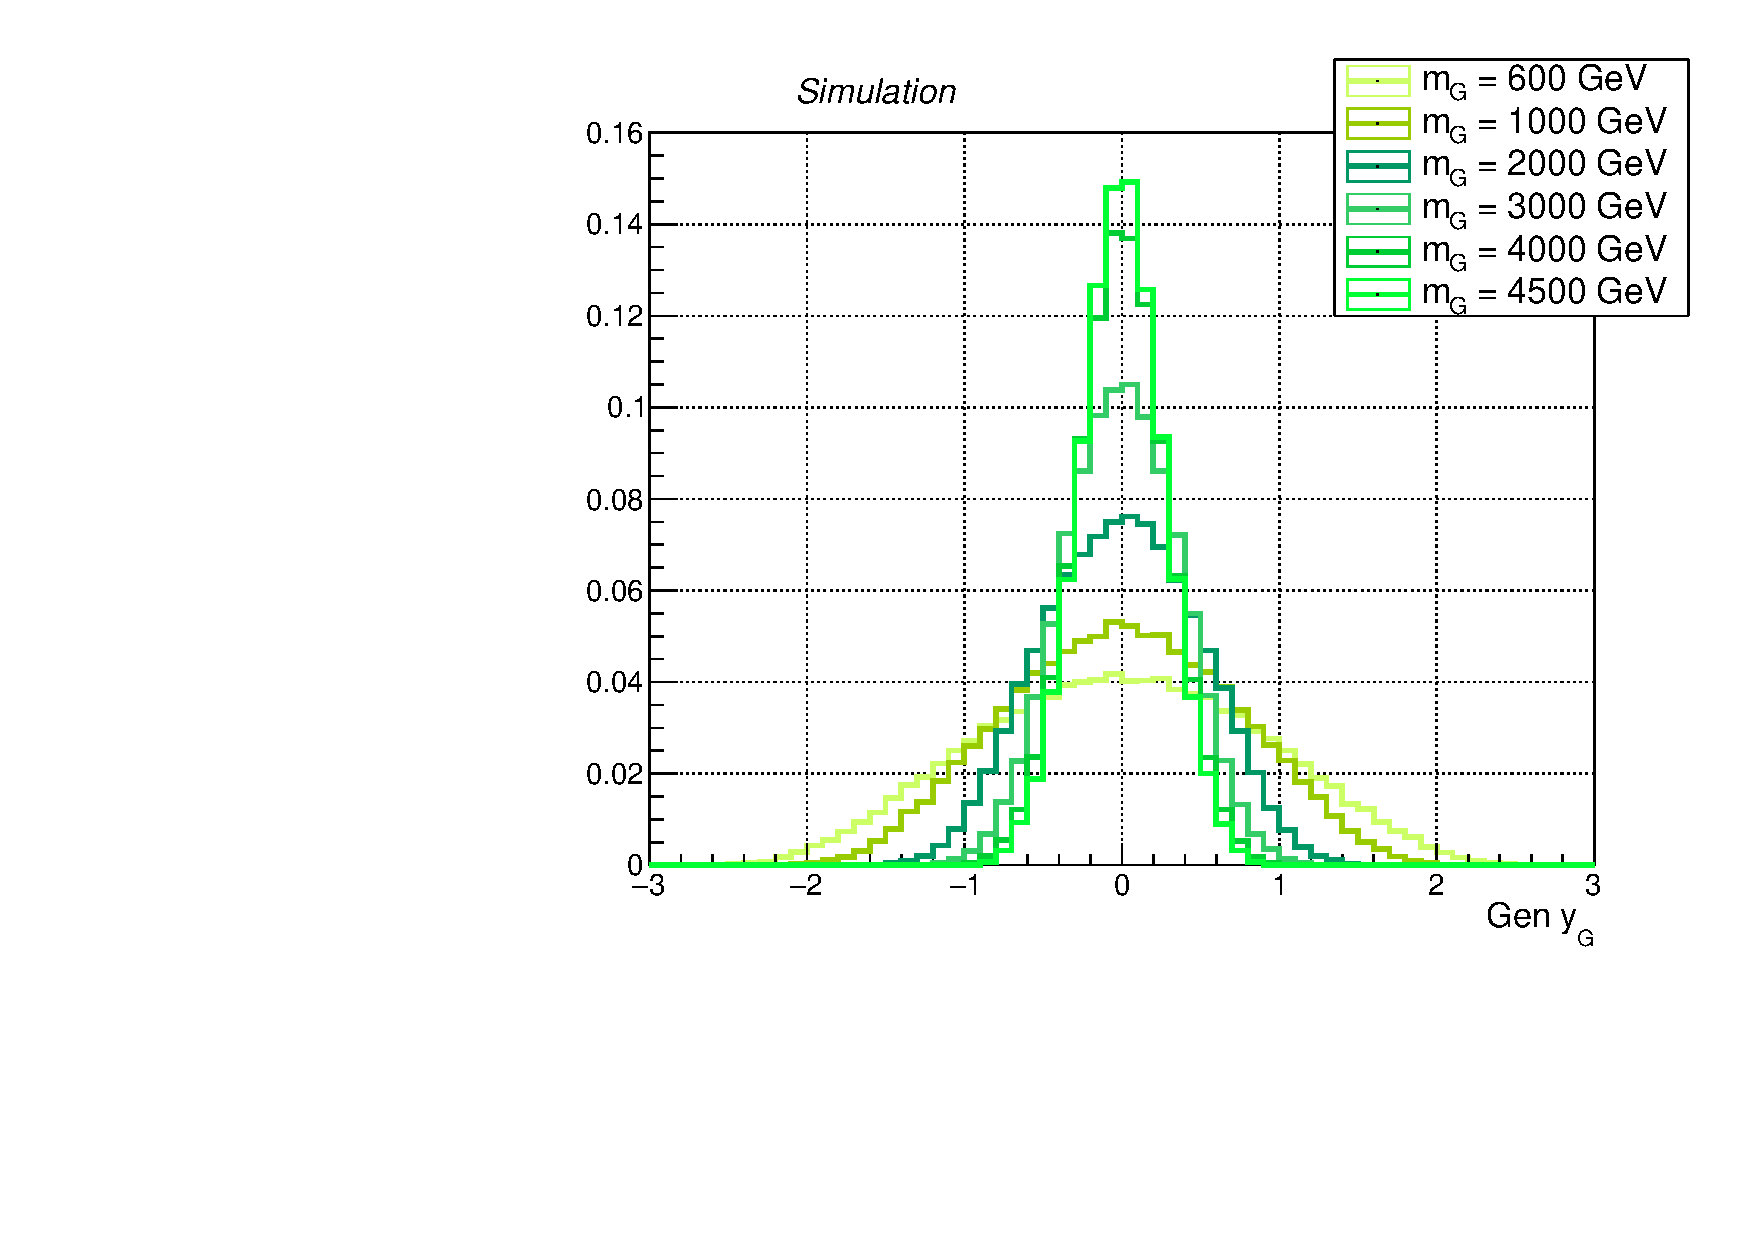
\includegraphics[width=.495\textwidth]{Gen_v9/XZZInv_g_XRapidity.pdf}%GenPhi1pt.pdf}
     %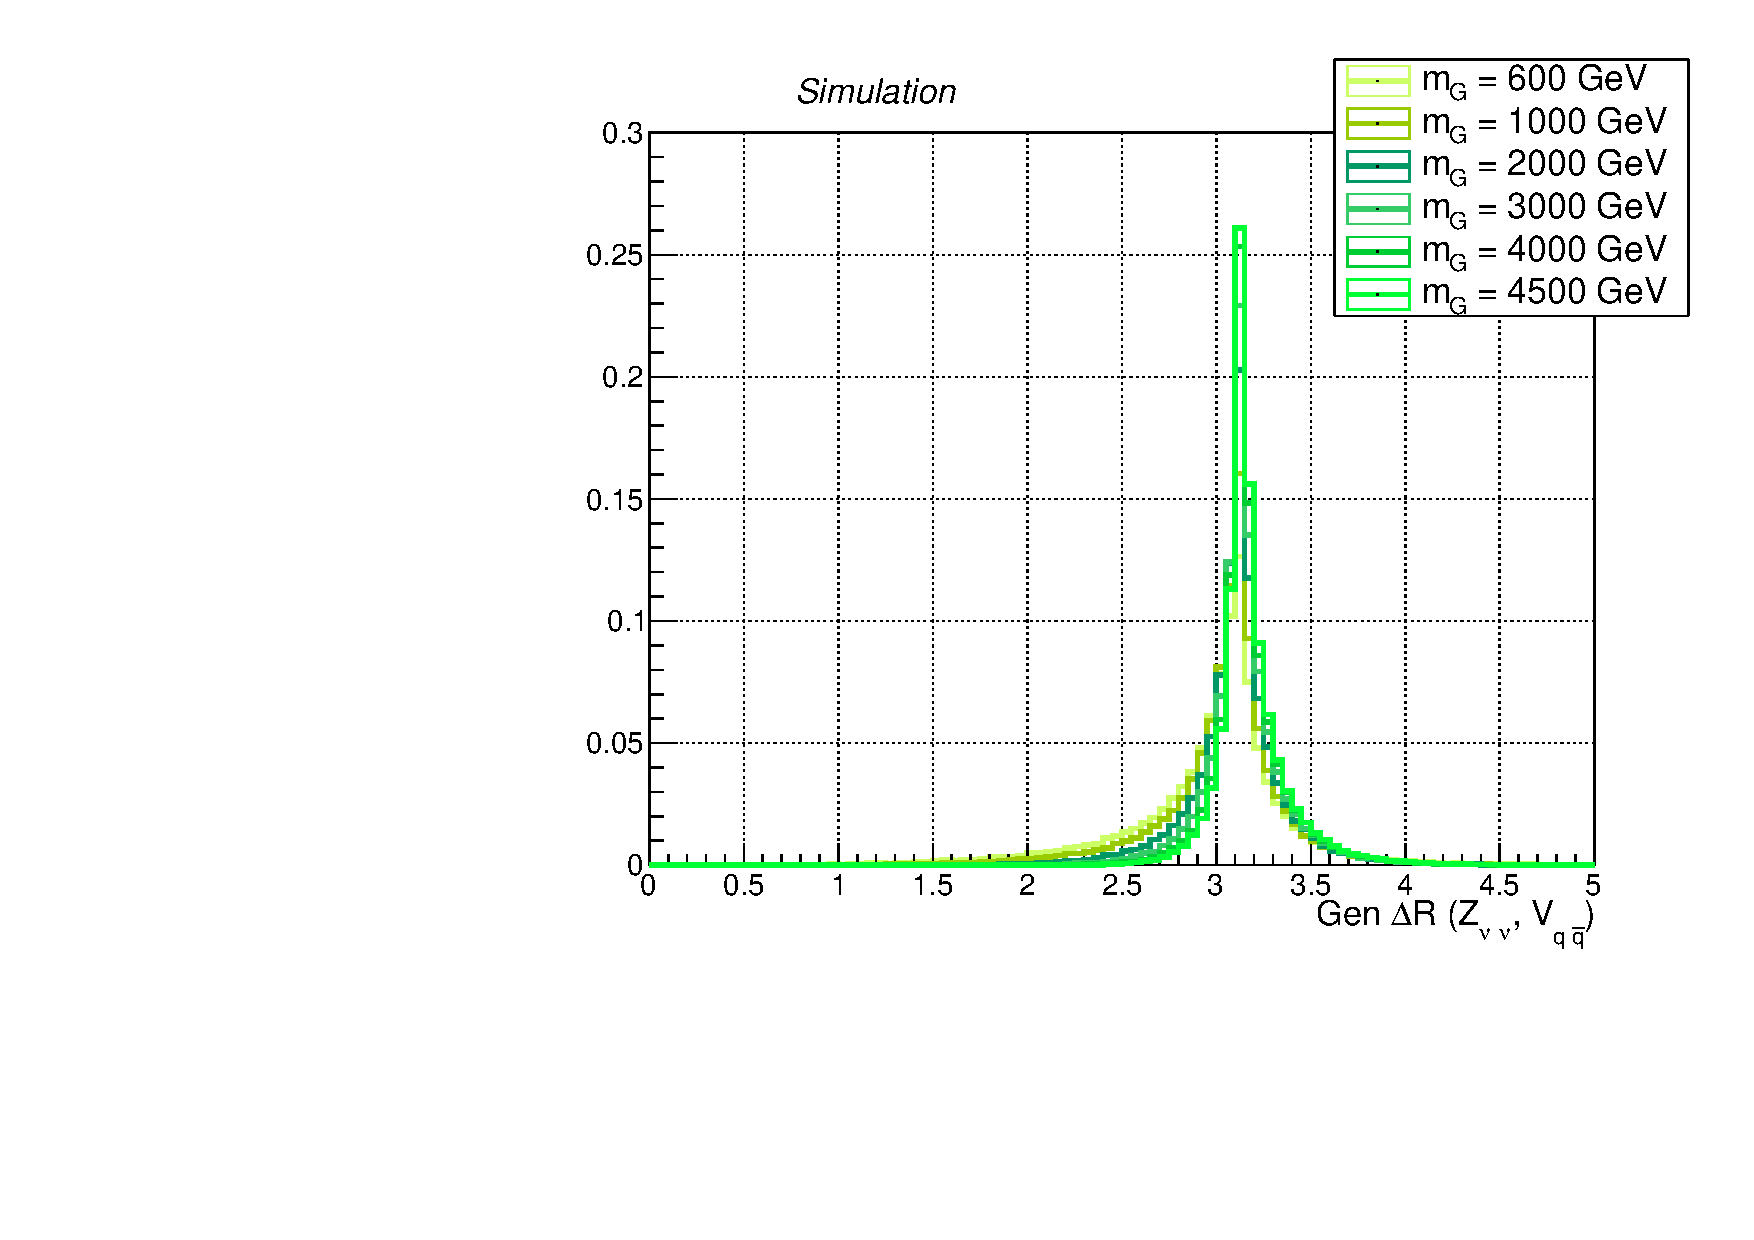
\includegraphics[width=.495\textwidth]{Gen_v9/XZZInv_g_VZDR.pdf}%GenPhi1y.pdf}
     %\\
     %\includegraphics[width=.495\textwidth]{Gen_v7/g_ZLepMass.pdf}%GenZmass.pdf}
     %\includegraphics[width=.495\textwidth]{Gen_v7/g_ZHadMass.pdf}%GenHmass.pdf}
     \\
     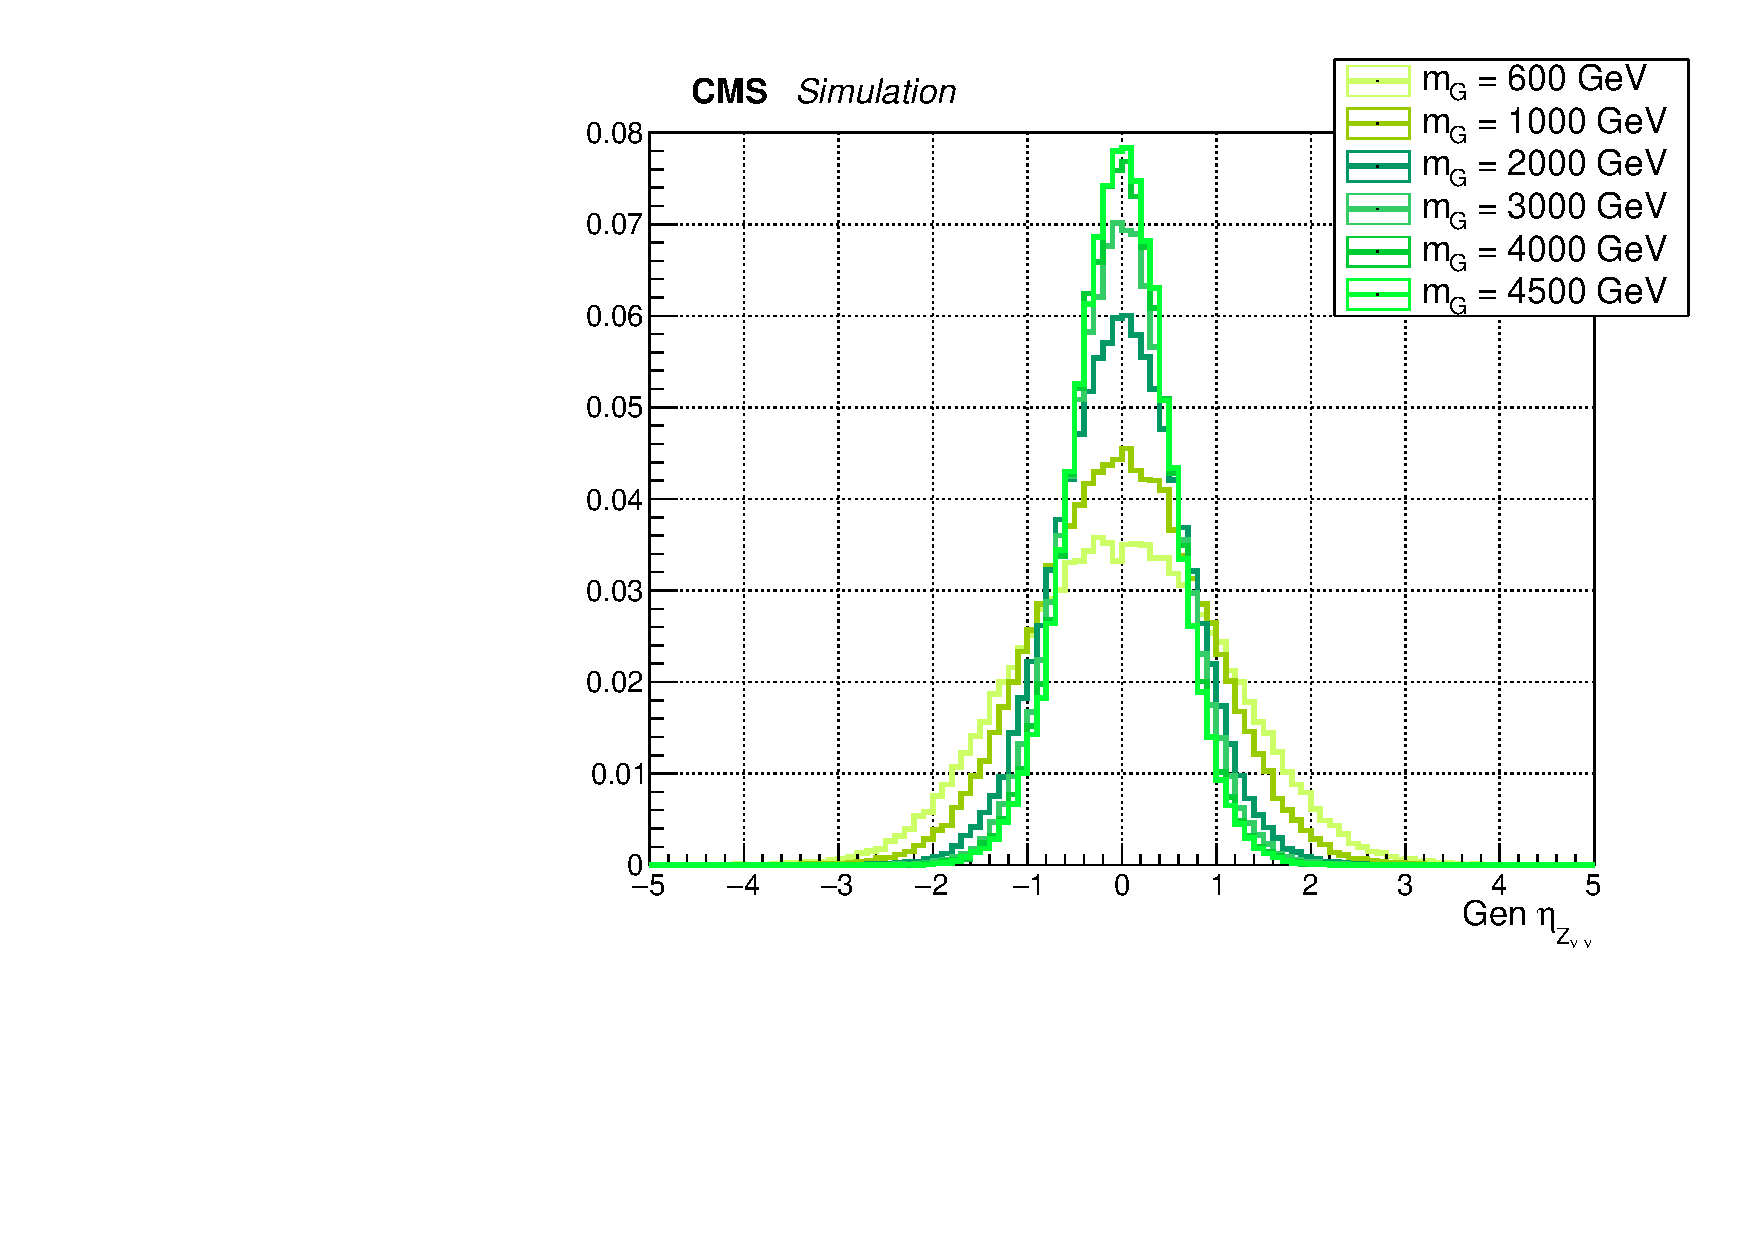
\includegraphics[width=.495\textwidth]{Gen_v9/XZZInv_g_ZLepEta.pdf}%GenZpt.pdf}
     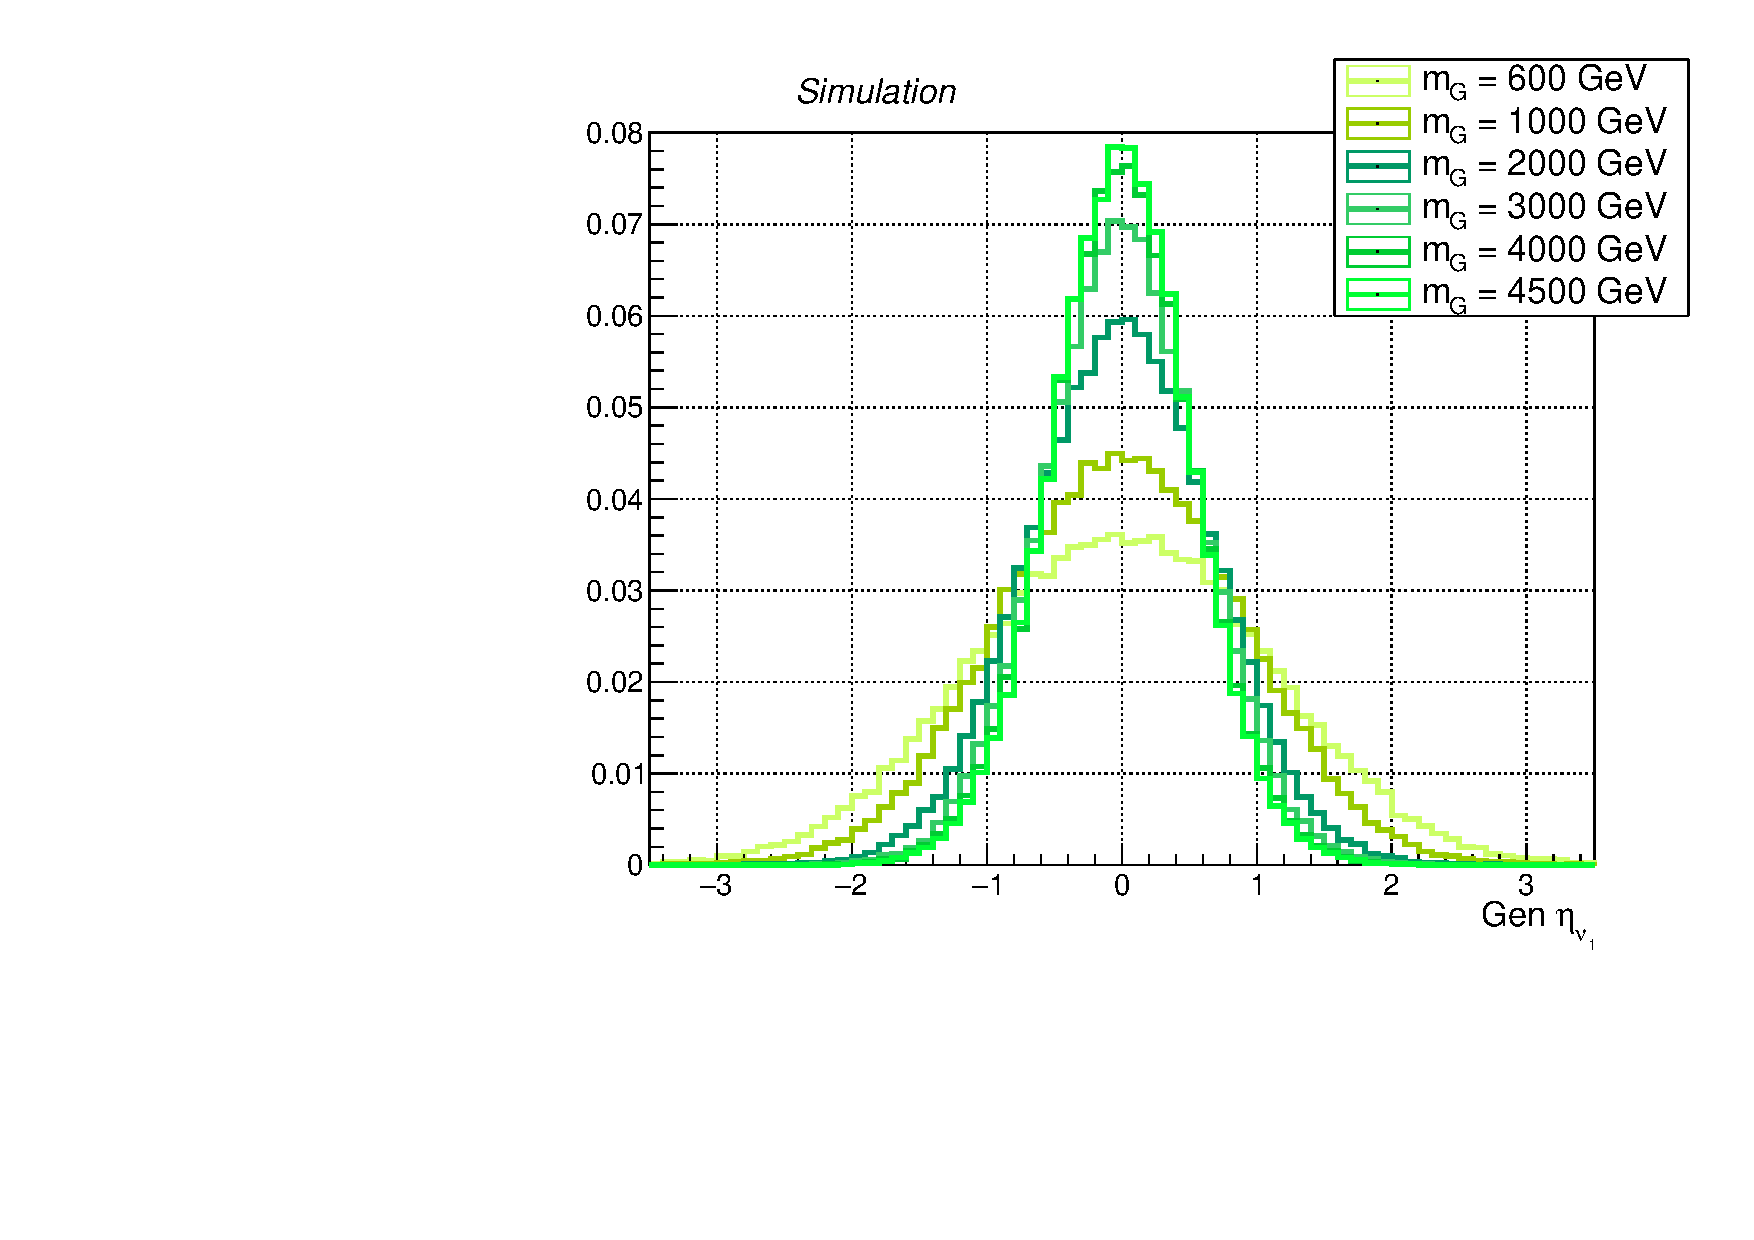
\includegraphics[width=.495\textwidth]{Gen_v9/XZZInv_g_Lep1Eta.pdf}%GenHpt.pdf}
     \\
     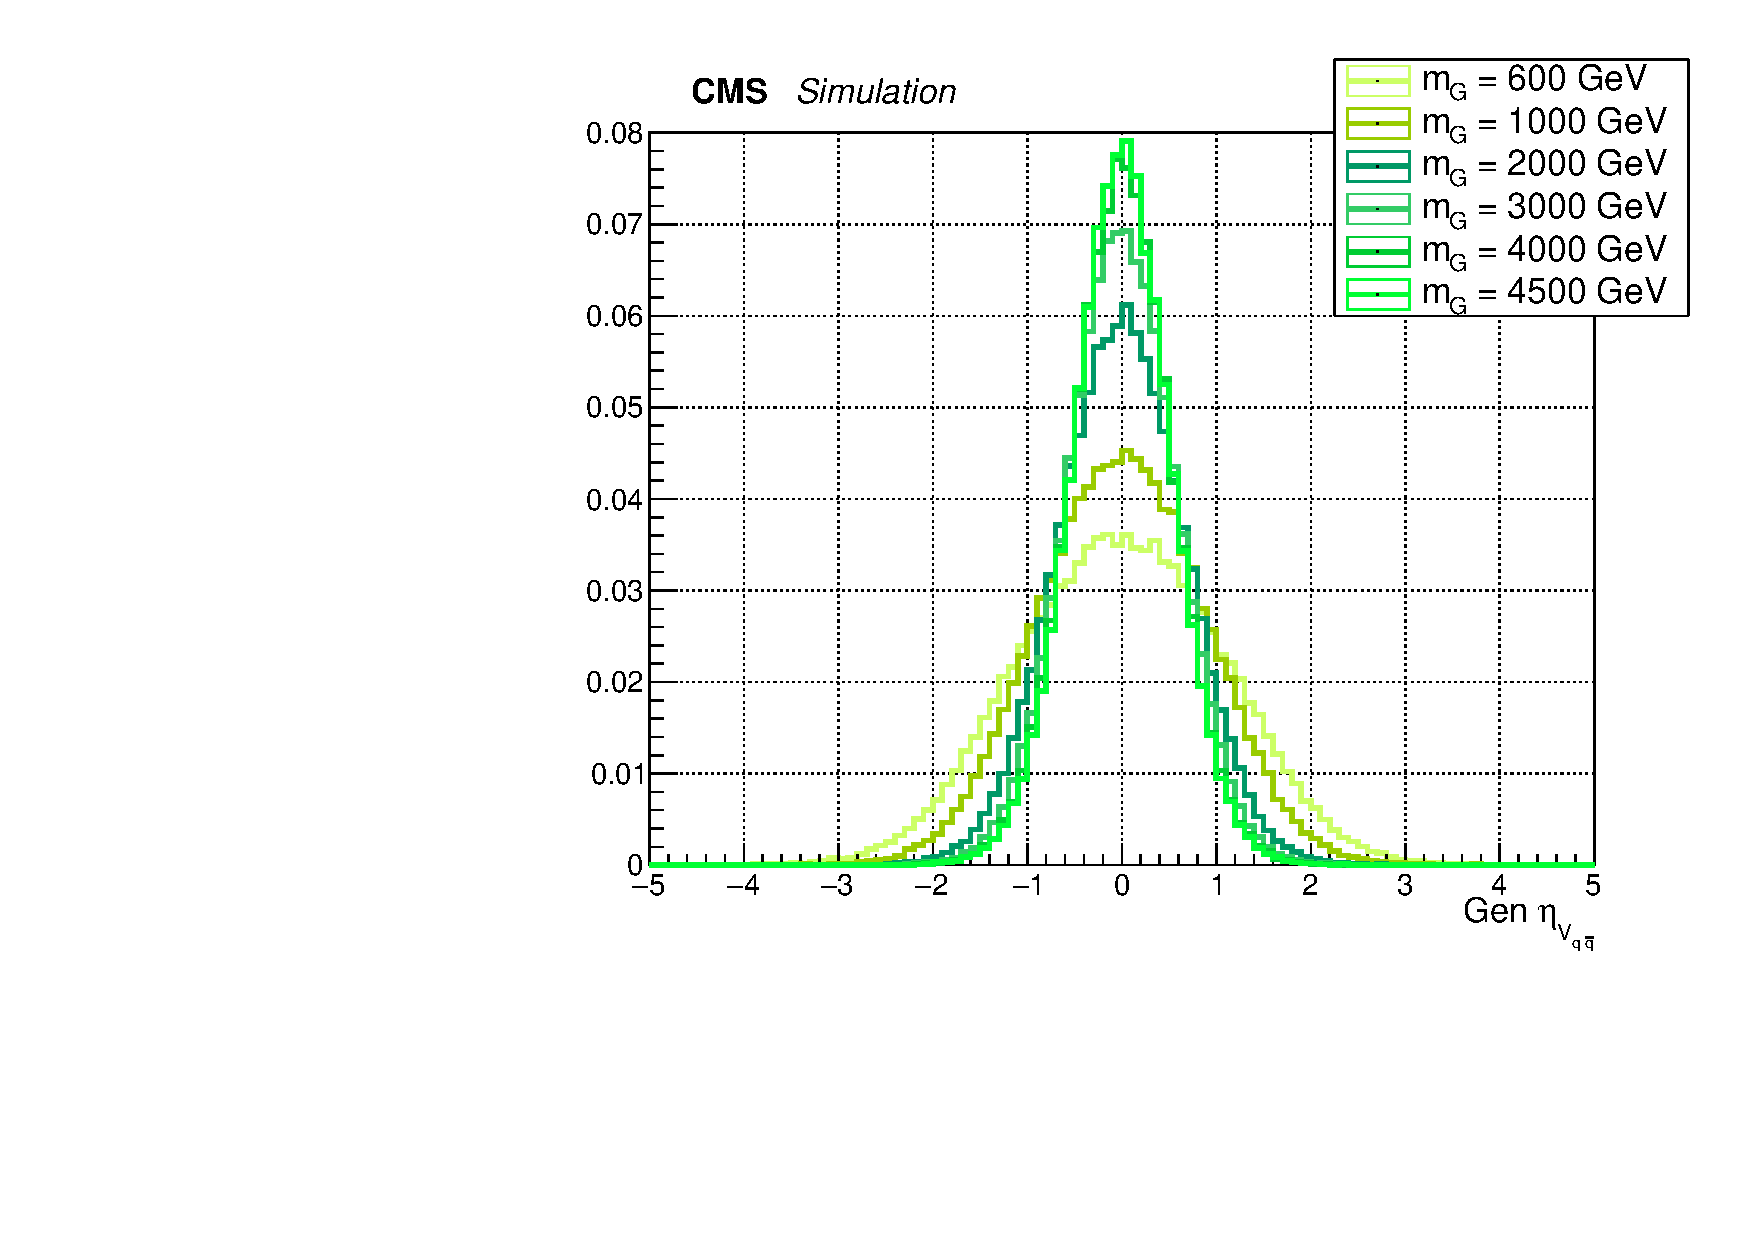
\includegraphics[width=.495\textwidth]{Gen_v9/XZZInv_g_VHadEta.pdf}%GenZdR.pdf}
     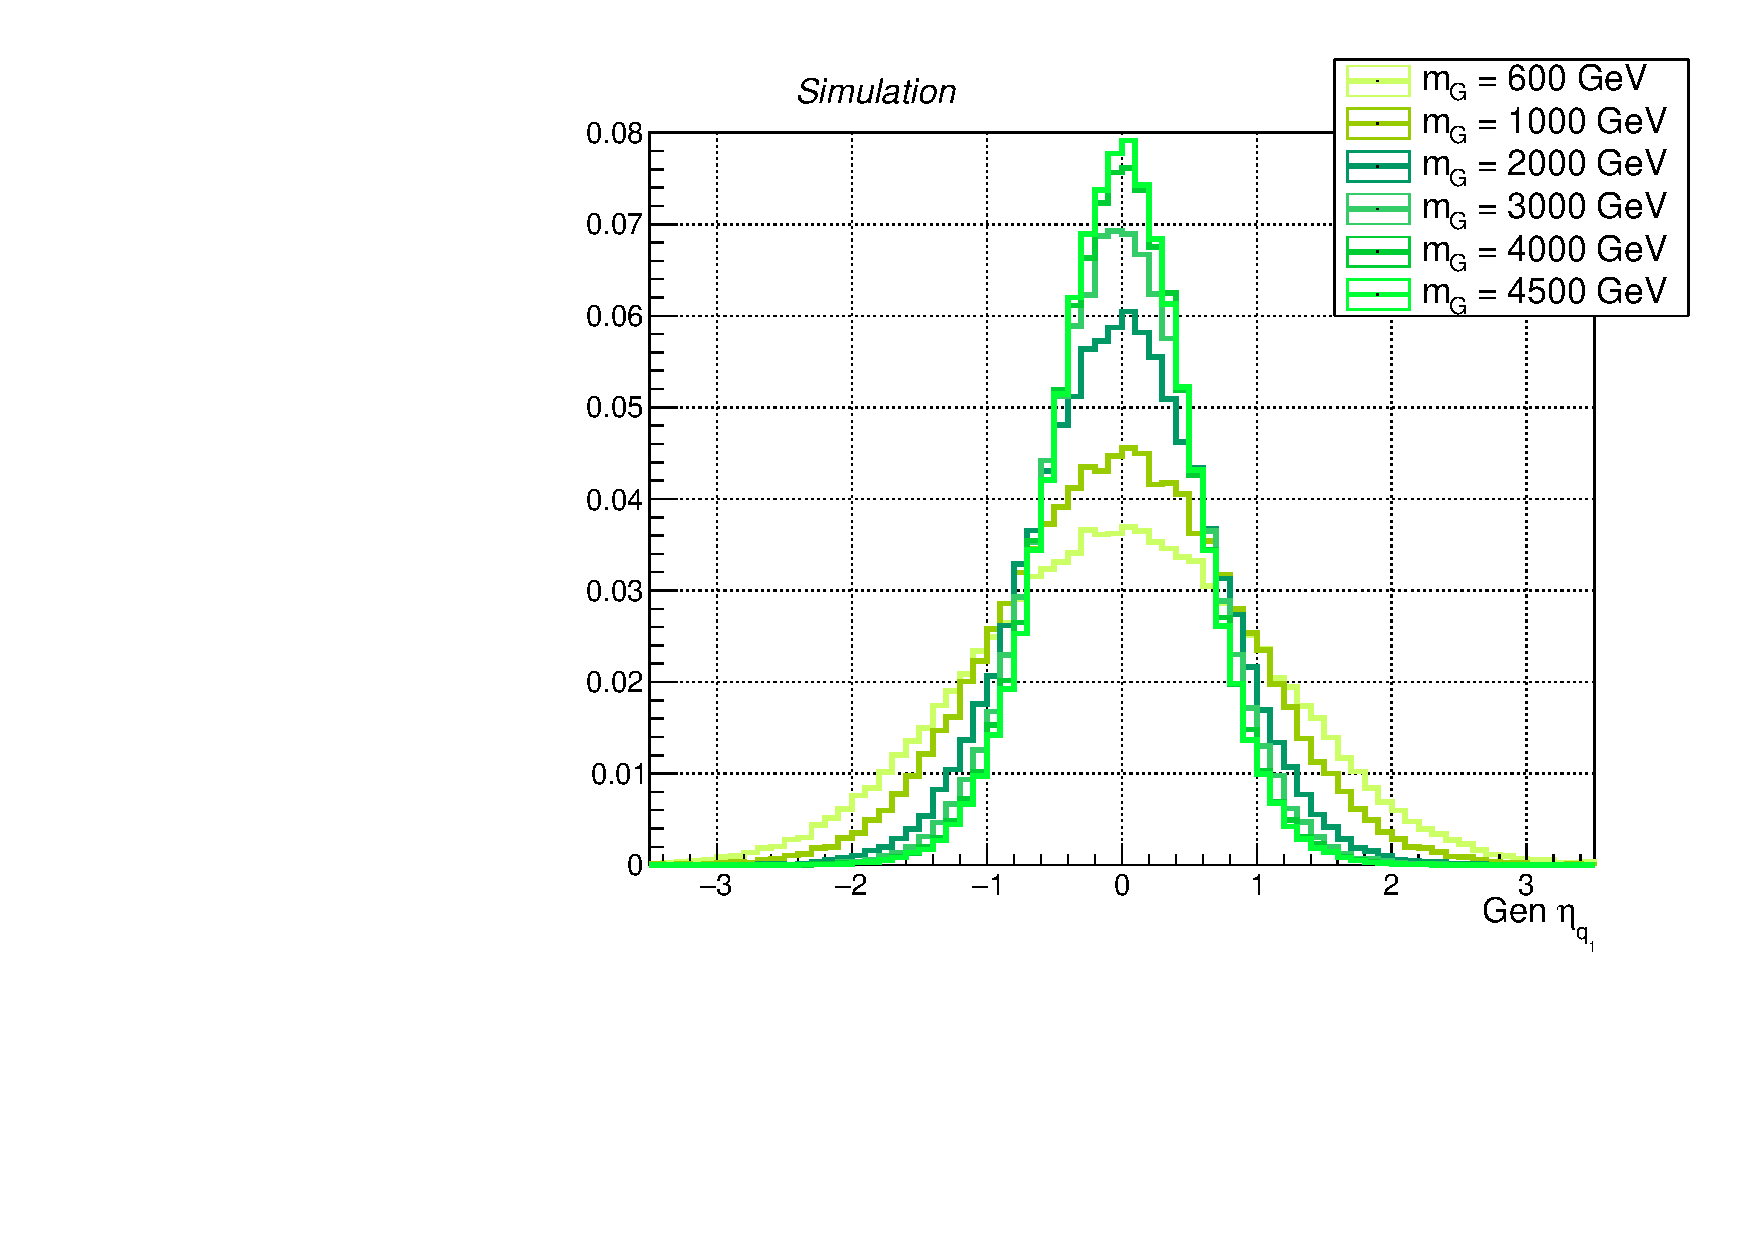
\includegraphics[width=.495\textwidth]{Gen_v9/XZZInv_g_Had1Eta.pdf}%GenHdR.pdf}
   \end{center}
   \caption{Main signal kinematic quantities at generation level after parton showering, for spin-2 Bulk Graviton signal, considering different mass hypoteses ($m_{\G} = 0.6, 1, 2, 3, 4, 4.5$ TeV). Top: graviton rapidity $\mathcal{Y}$. Center: pseudorapidity $\eta$ of the invisibly decaying \Z, and pseudorapidity of the leading neutrino. Bottom: pseudorapidity $\eta$ of the hadronically decaying \Z, and pseudorapidity of the leading quark.}
   \label{fig:genGravSignal2}
 \end{figure}

 \begin{figure}[!htb]
   \begin{center}
     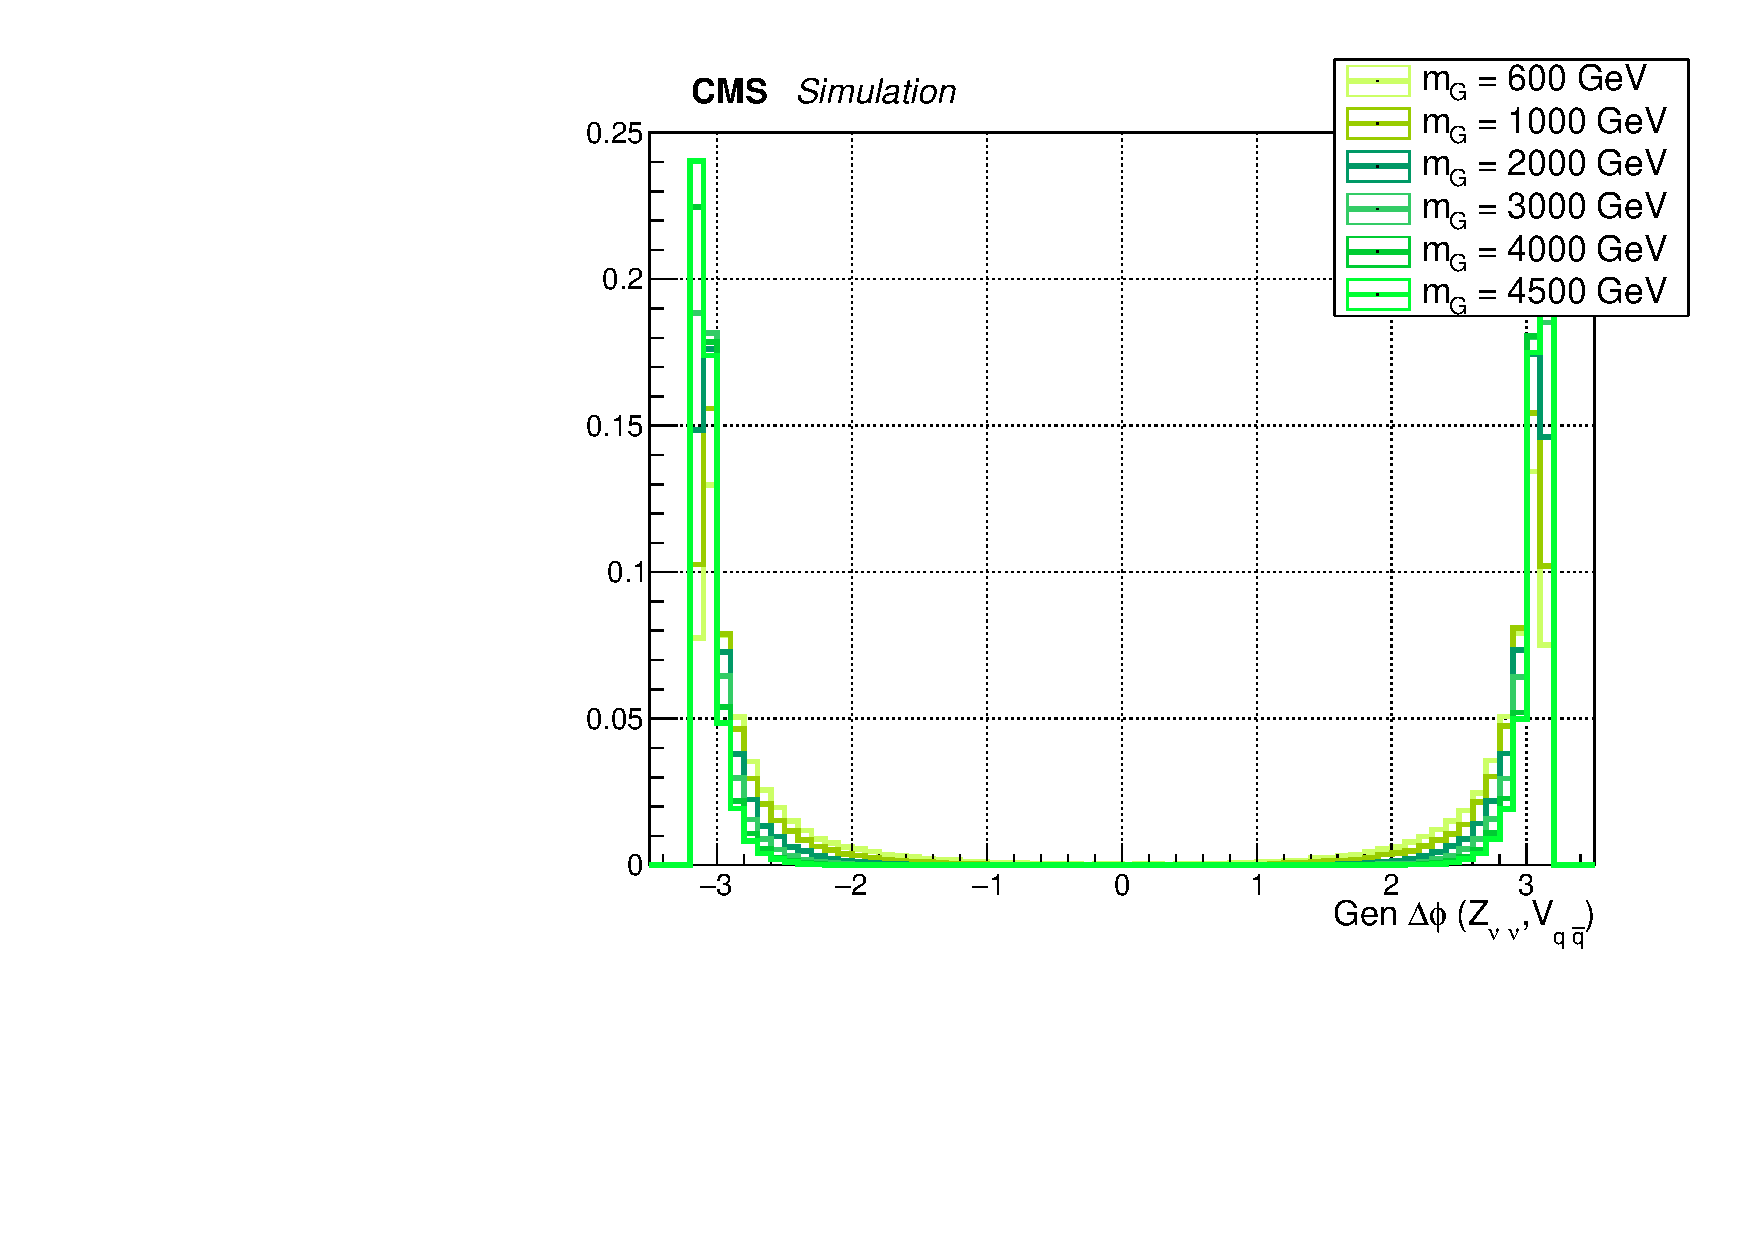
\includegraphics[width=.495\textwidth]{Gen_v9/XZZInv_g_VZDPhi.pdf}%GenPhi1pt.pdf}
     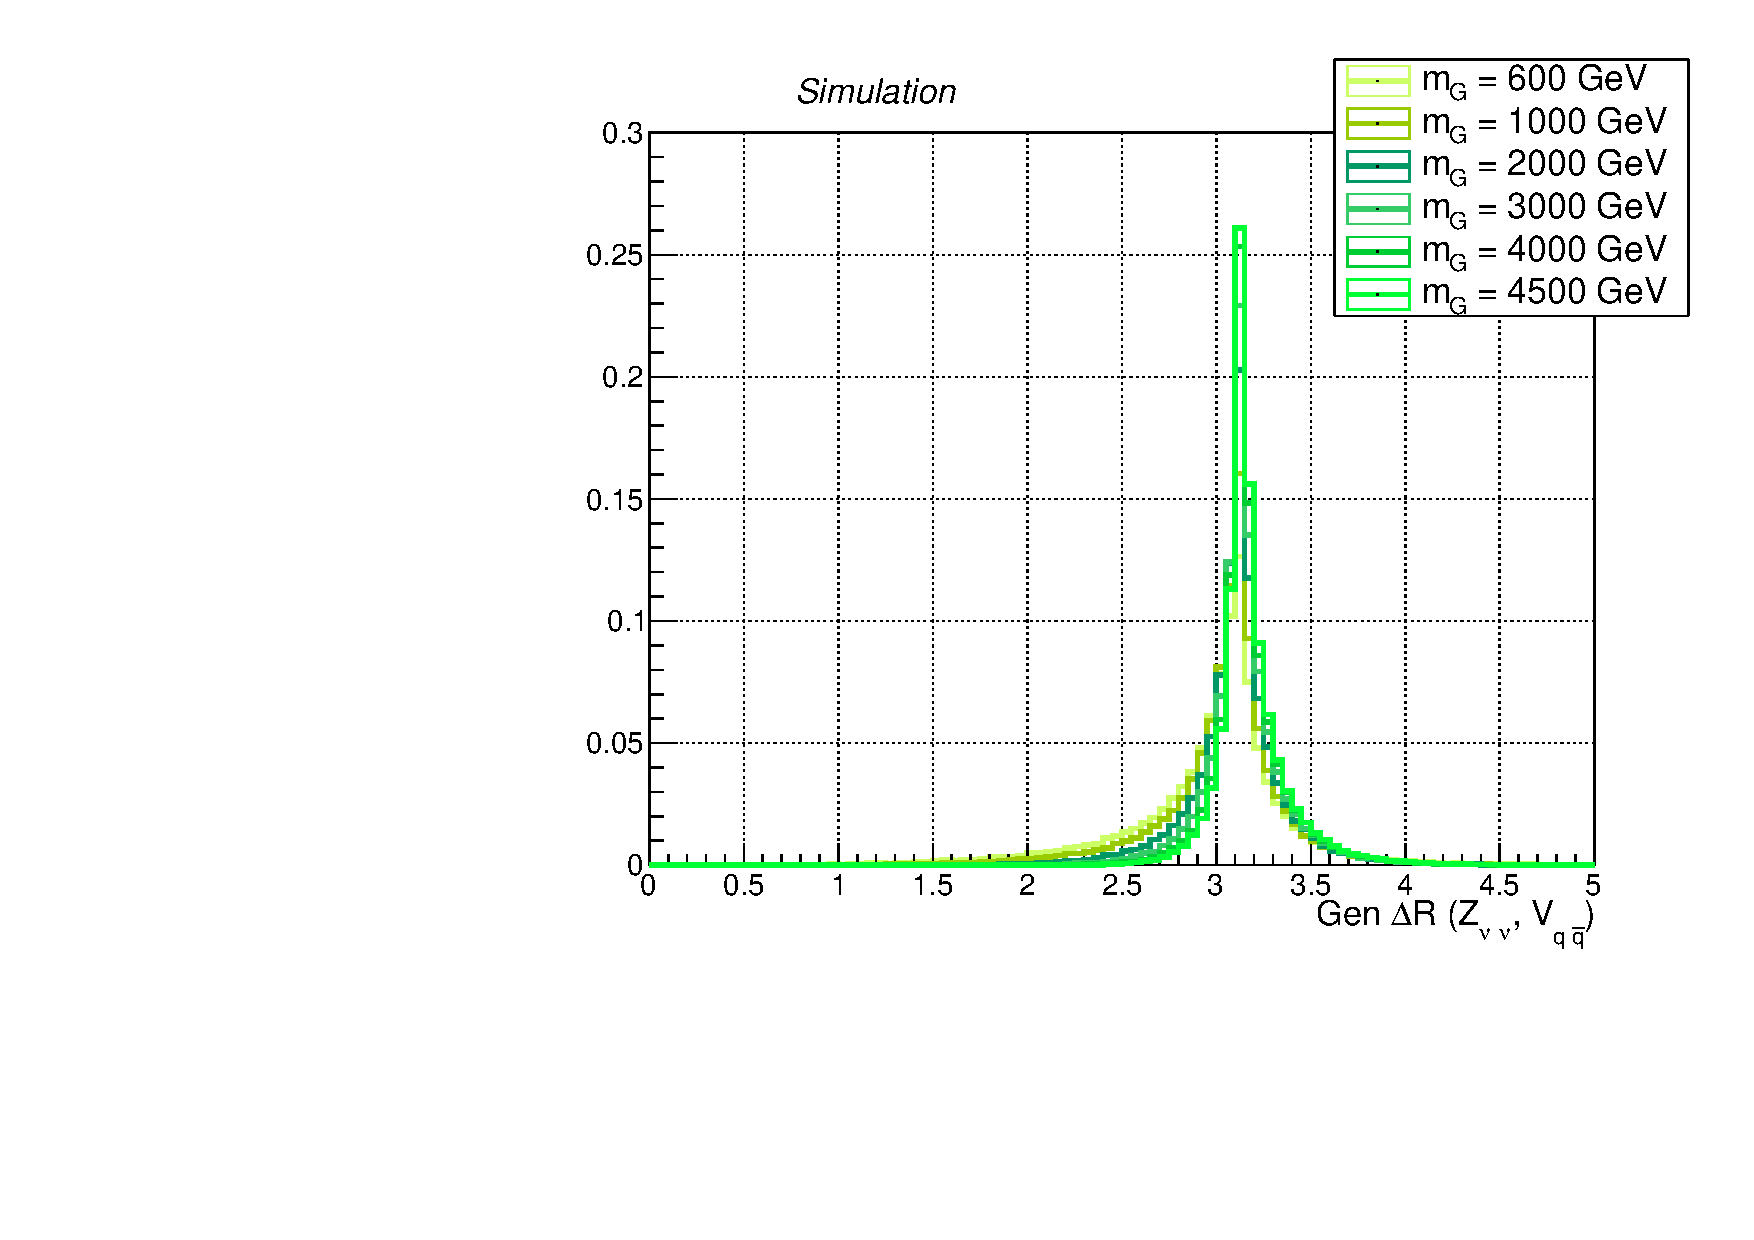
\includegraphics[width=.495\textwidth]{Gen_v9/XZZInv_g_VZDR.pdf}%GenPhi1y.pdf}
     %\\
     %\includegraphics[width=.495\textwidth]{Gen_v7/g_ZLepMass.pdf}%GenZmass.pdf}
     %\includegraphics[width=.495\textwidth]{Gen_v7/g_ZHadMass.pdf}%GenHmass.pdf}
     \\
     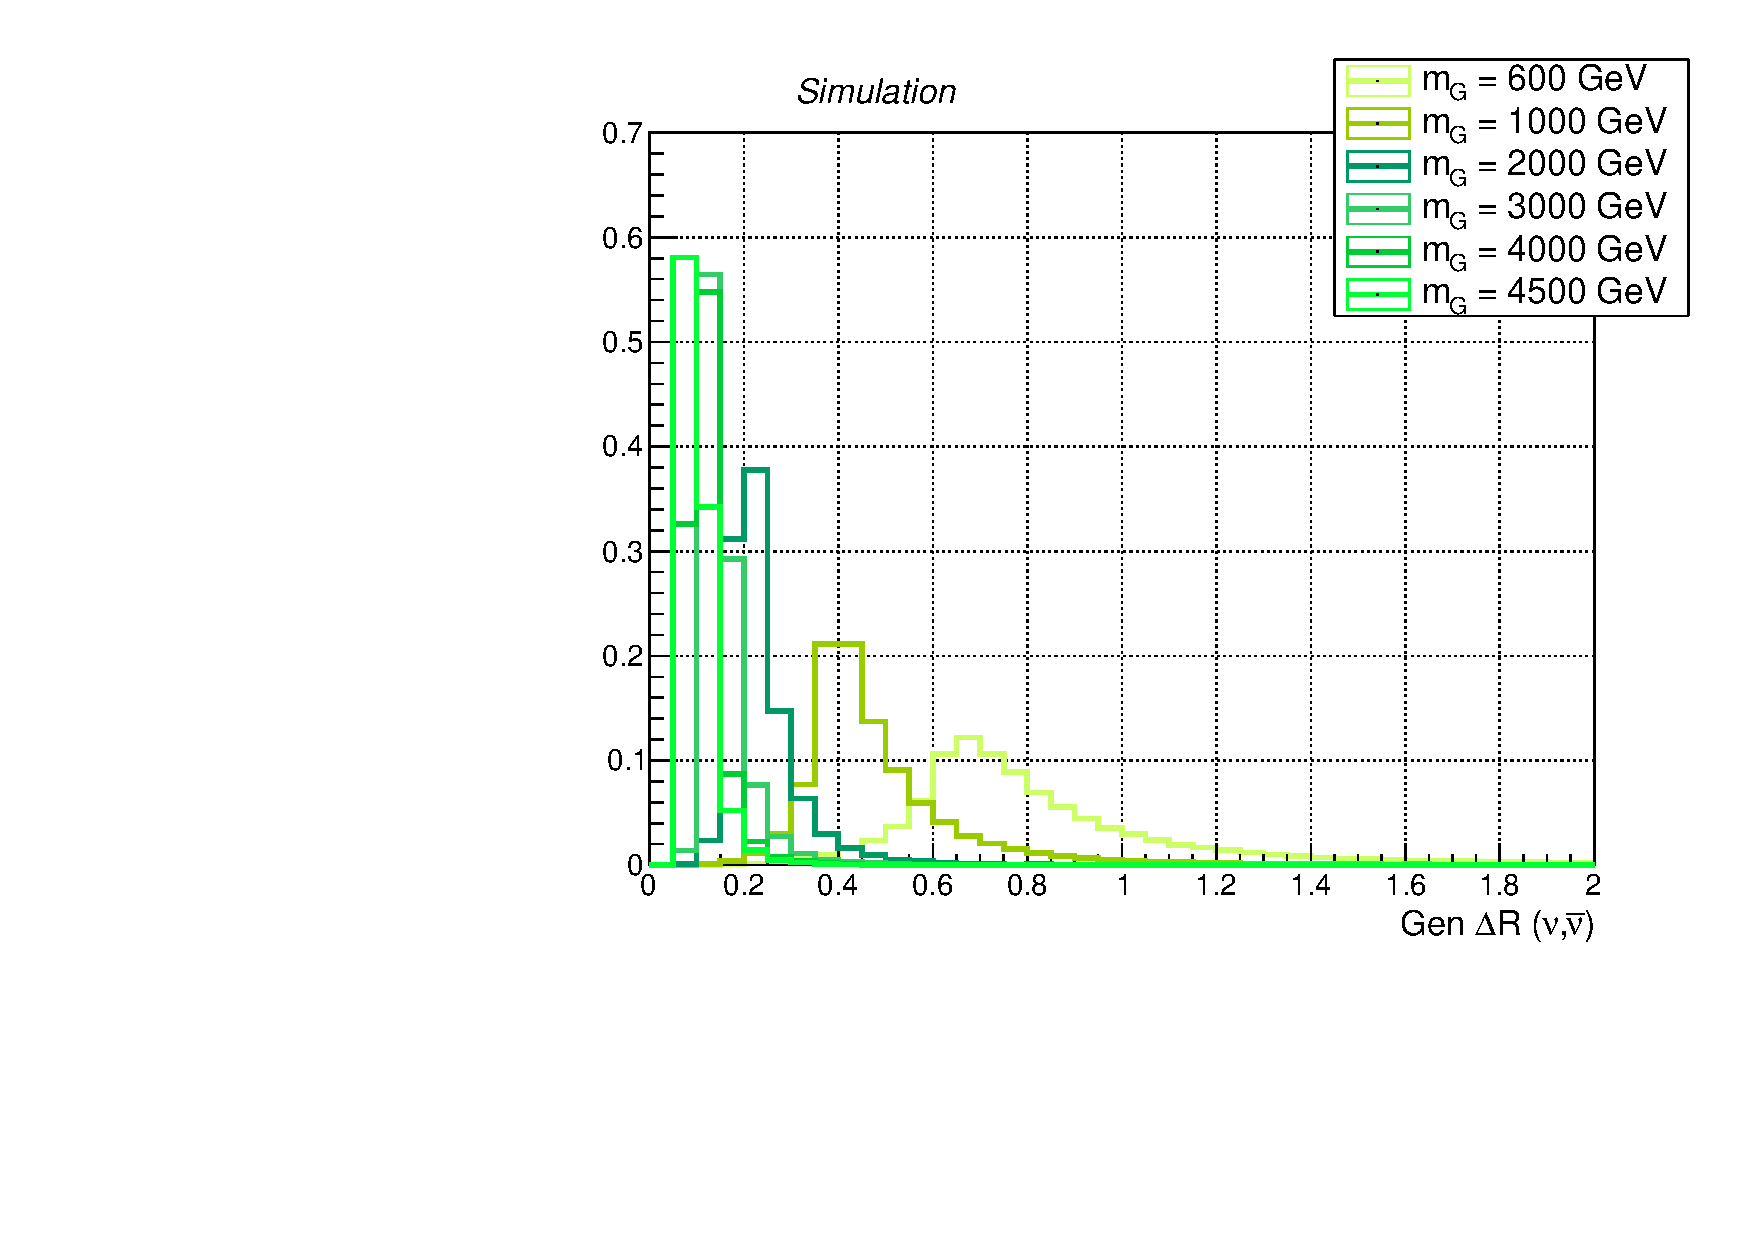
\includegraphics[width=.495\textwidth]{Gen_v9/XZZInv_g_LepDR.pdf}%GenZpt.pdf}
     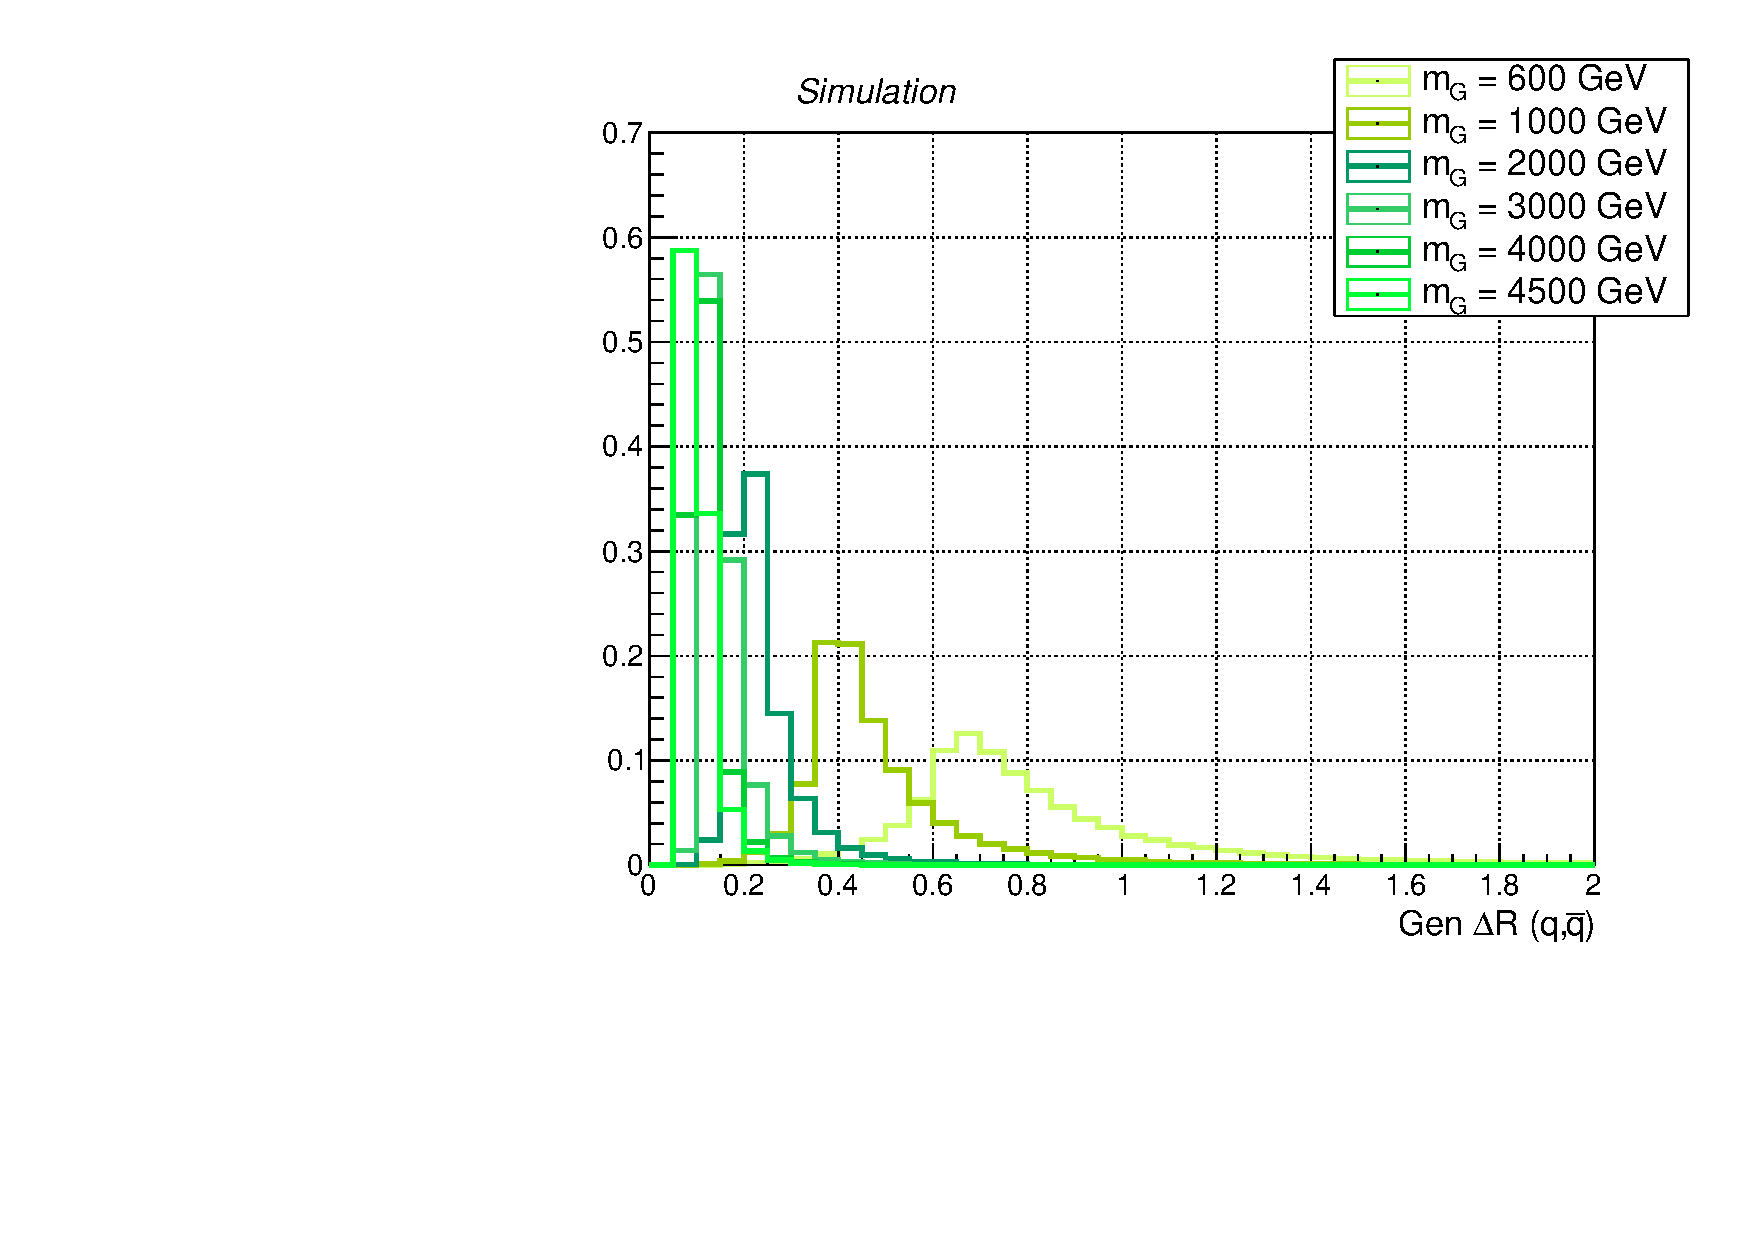
\includegraphics[width=.495\textwidth]{Gen_v9/XZZInv_g_HadDR.pdf}%GenHpt.pdf}
     \\
     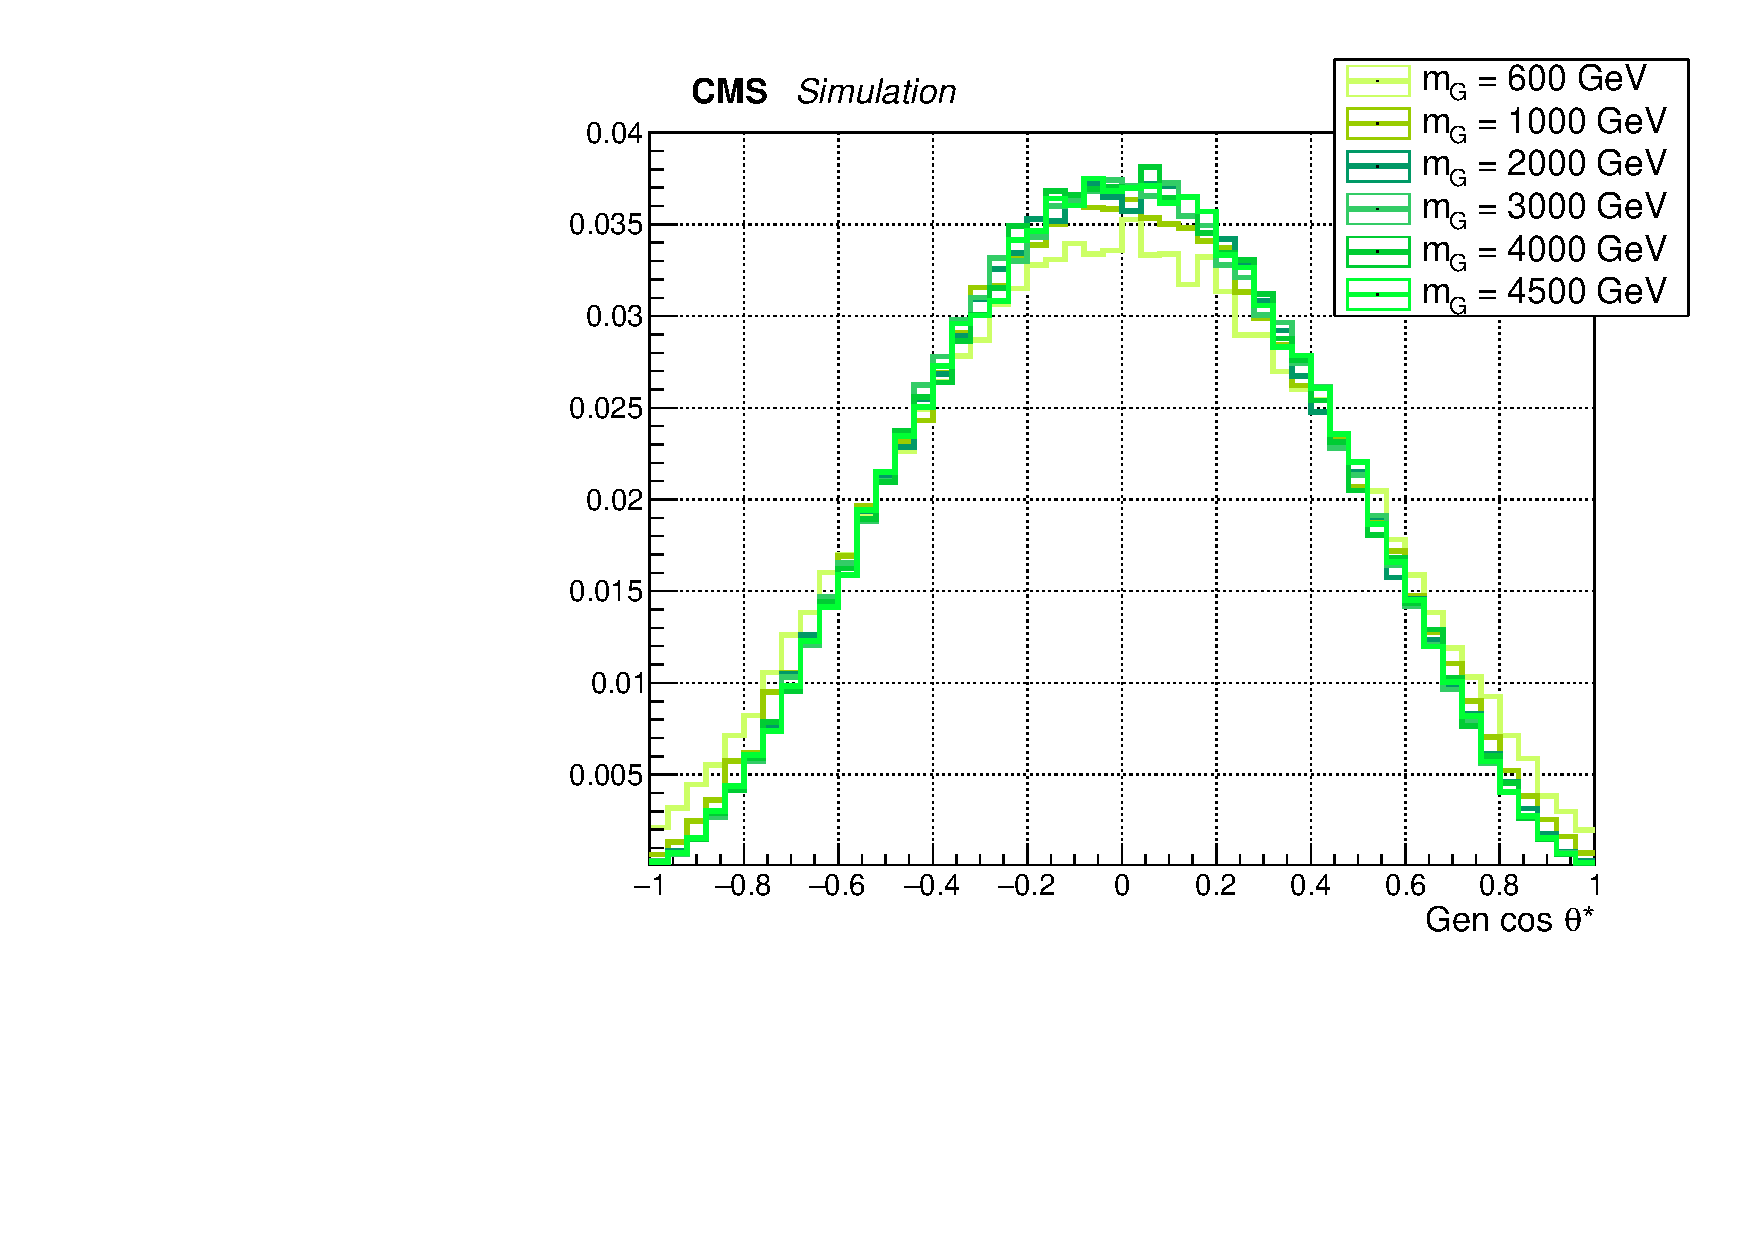
\includegraphics[width=.495\textwidth]{Gen_v9/XZZInv_g_CosThetaStar.pdf}%GenZdR.pdf}
     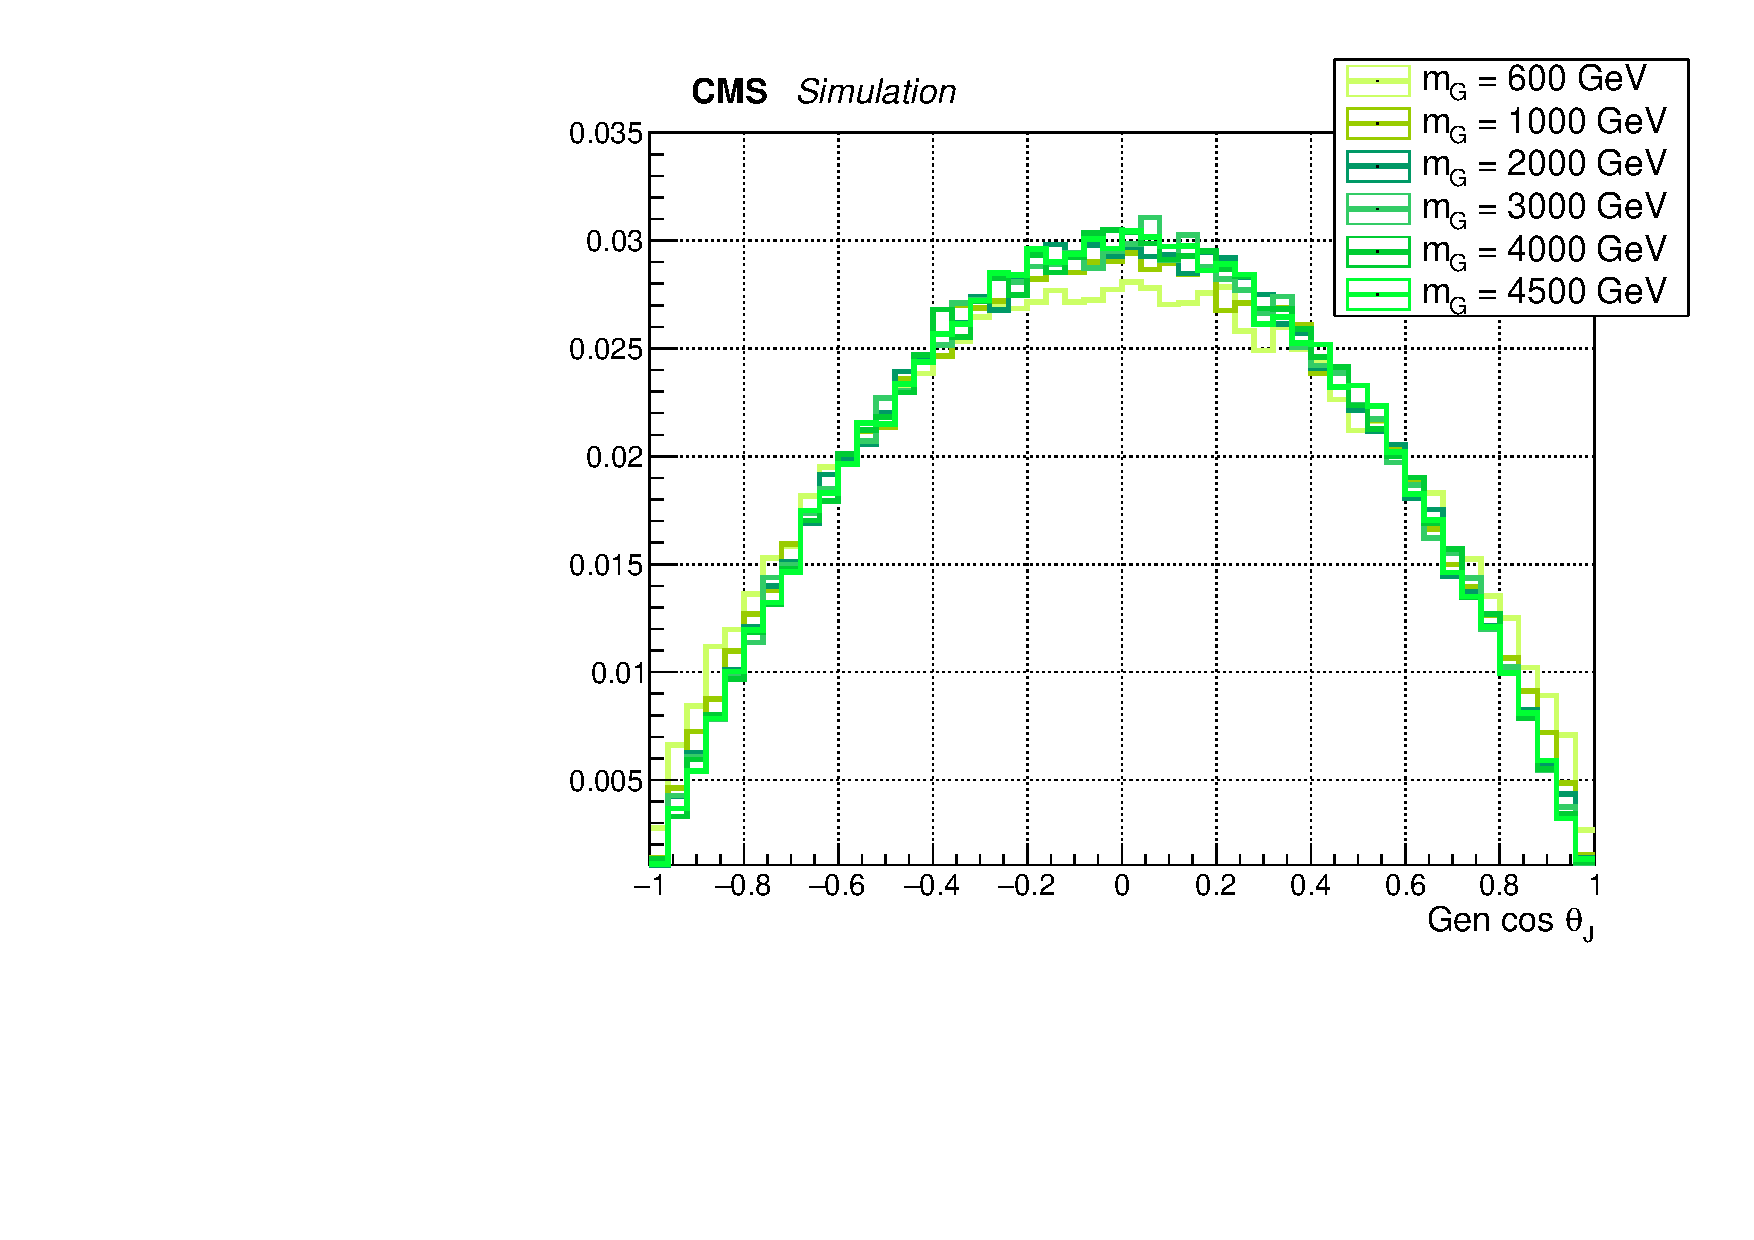
\includegraphics[width=.495\textwidth]{Gen_v9/XZZInv_g_CosThetaJ.pdf}%GenHdR.pdf}
   \end{center}
   \caption{Main signal kinematic quantities at generation level after parton showering, for spin-2 Bulk Graviton signal, considering different mass hypoteses ($m_{\G} = 0.6, 1, 2, 3, 4, 4.5$ TeV). Top: angular separation in the transverse plane $\Delta \phi$ (left) and solid angle $\Delta R$ (right) between leptonic \Z and hadronic \Z. Center: solid angle between the neutrinos and the quarks. Bottom: distribution of $\cos{\theta}^{*}$ and $\cos{\theta}_{J}$ (described in text).}
   \label{fig:genGravSignal3}
 \end{figure}

 \begin{figure}[!htb]
   \begin{center}
     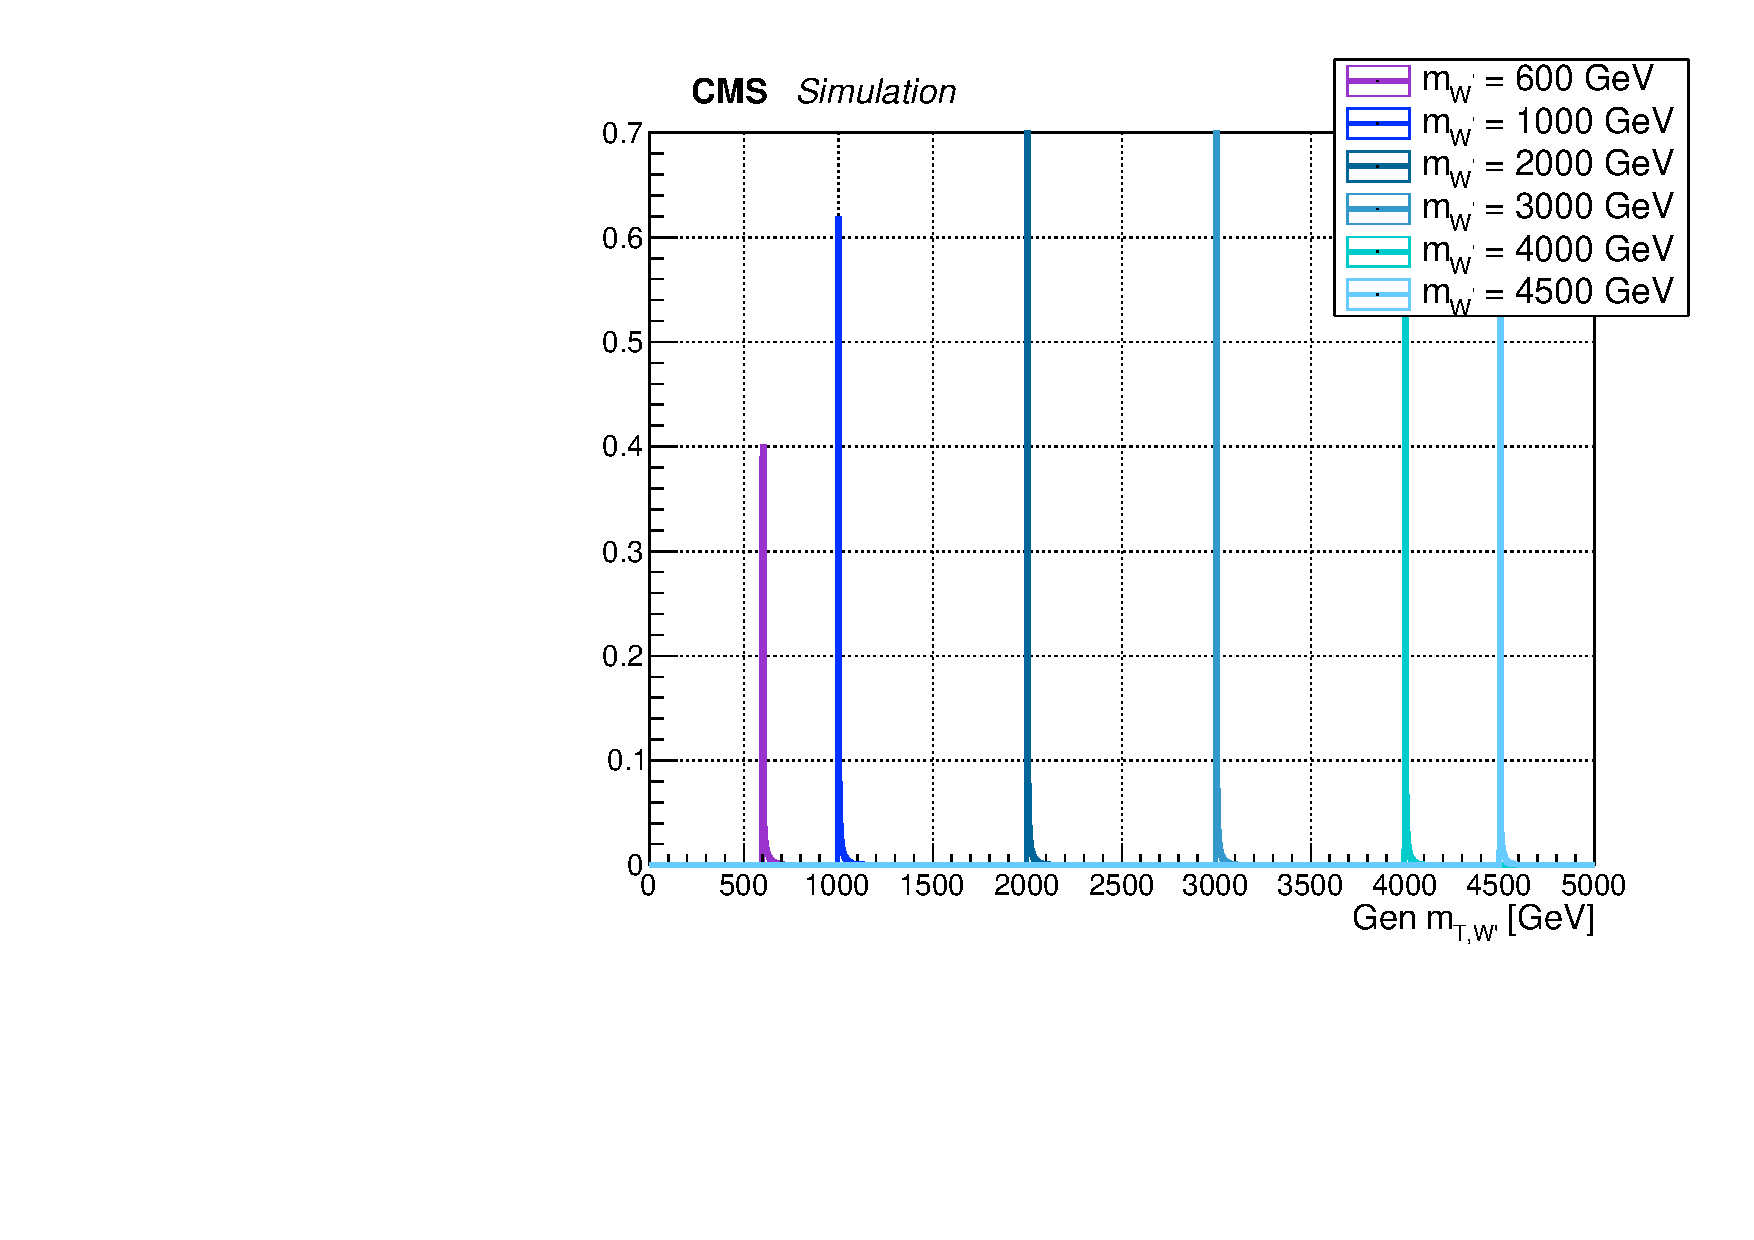
\includegraphics[width=.495\textwidth]{Gen_v9/XWZInv_g_XMT.pdf}%GenPhi1pt.pdf}
     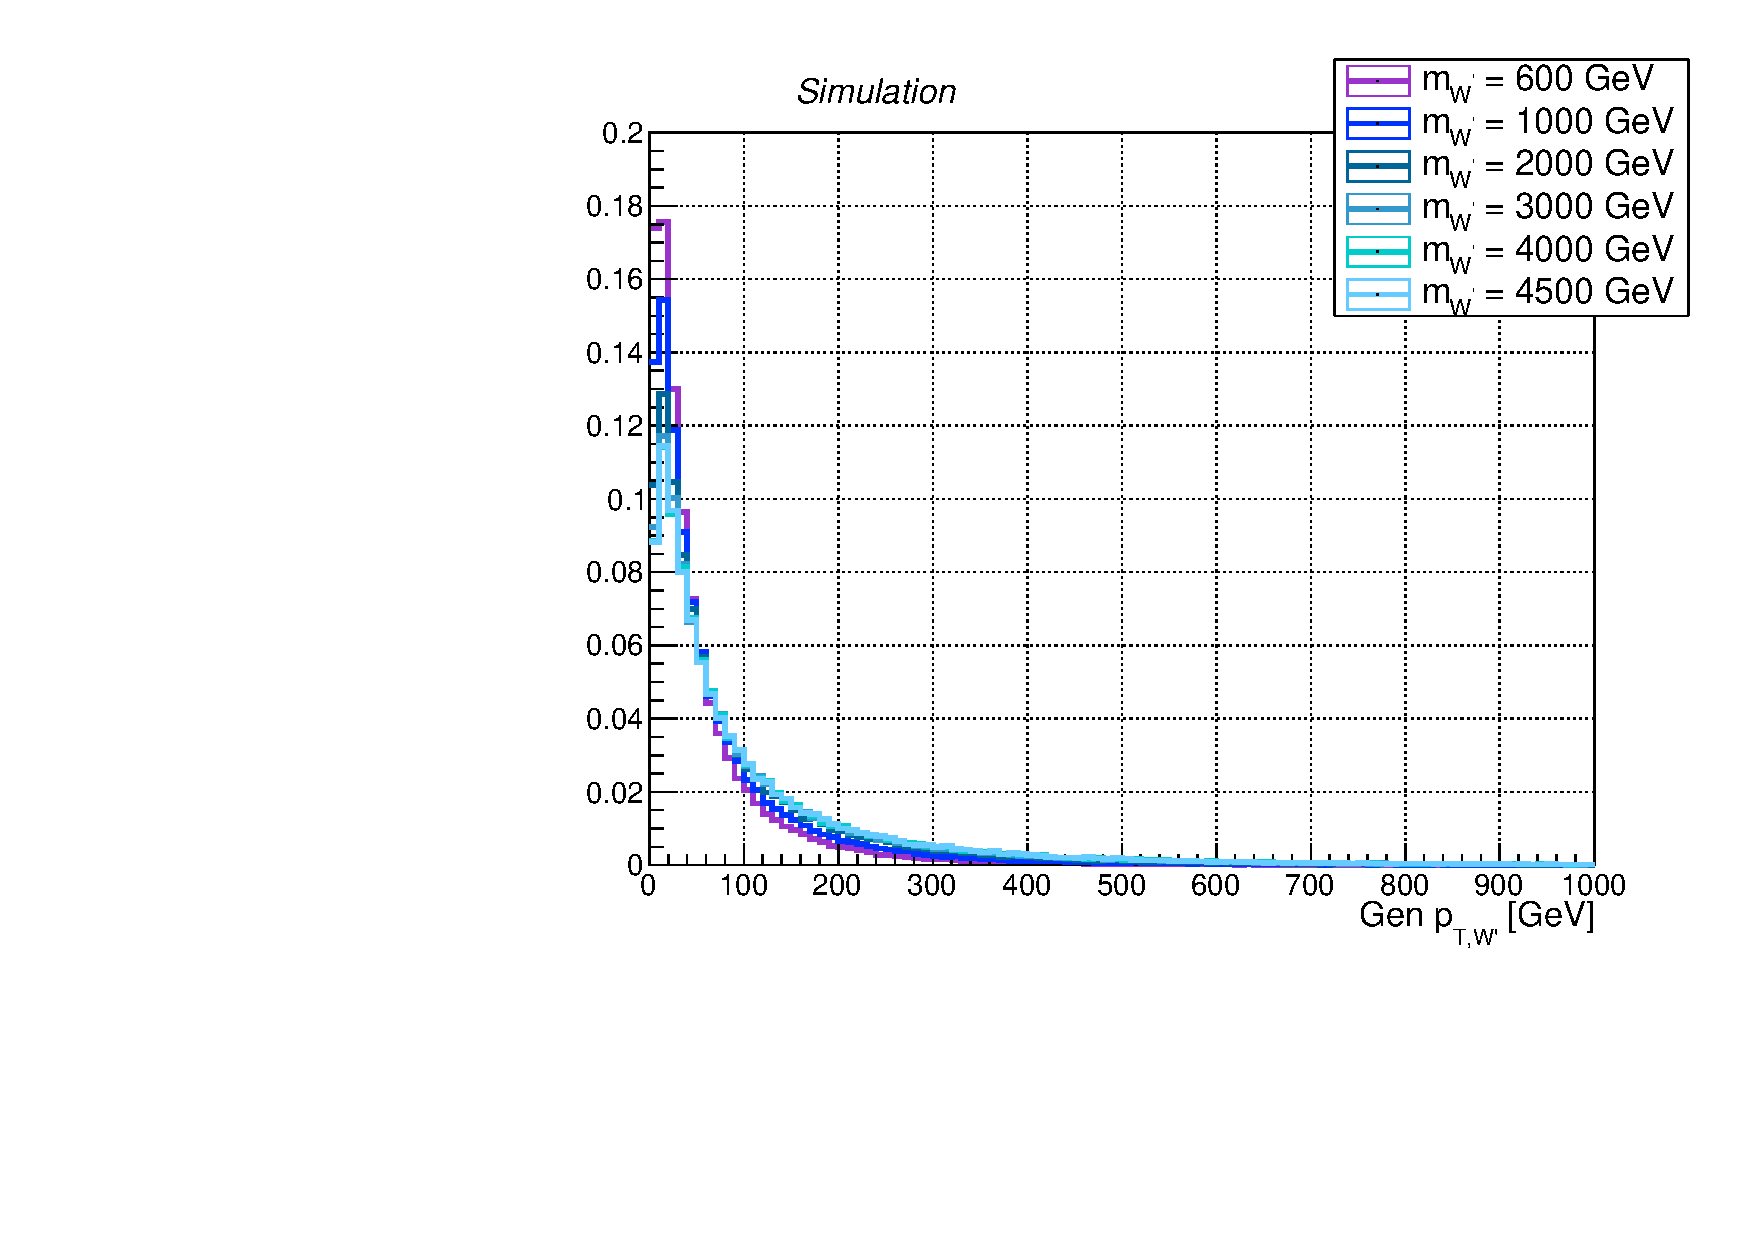
\includegraphics[width=.495\textwidth]{Gen_v9/XWZInv_g_XPt.pdf}%GenPhi1y.pdf}
     %\\
     %\includegraphics[width=.495\textwidth]{Gen_v7/g_ZLepMass.pdf}%GenZmass.pdf}
     %\includegraphics[width=.495\textwidth]{Gen_v7/g_ZHadMass.pdf}%GenHmass.pdf}
     \\
     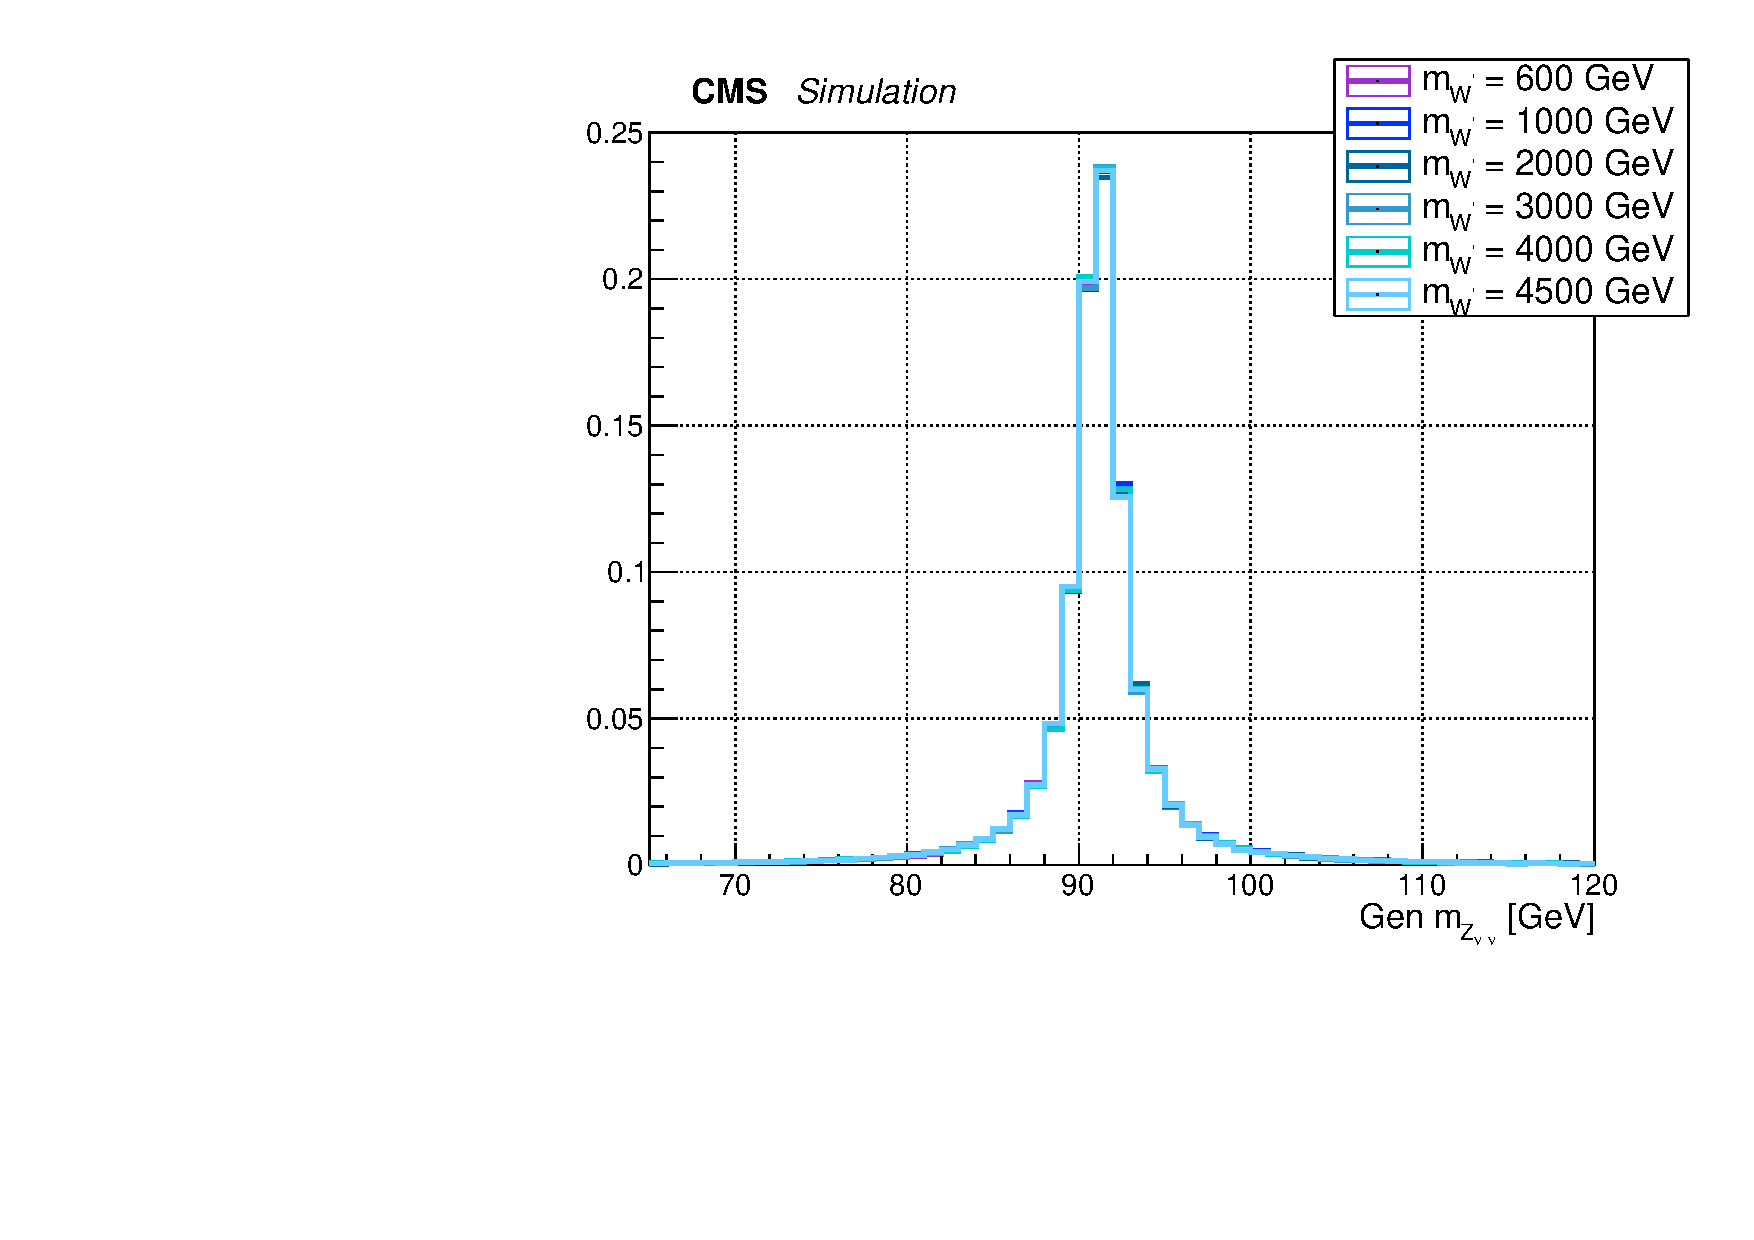
\includegraphics[width=.495\textwidth]{Gen_v9/XWZInv_g_ZLepMass.pdf}%GenZpt.pdf}
     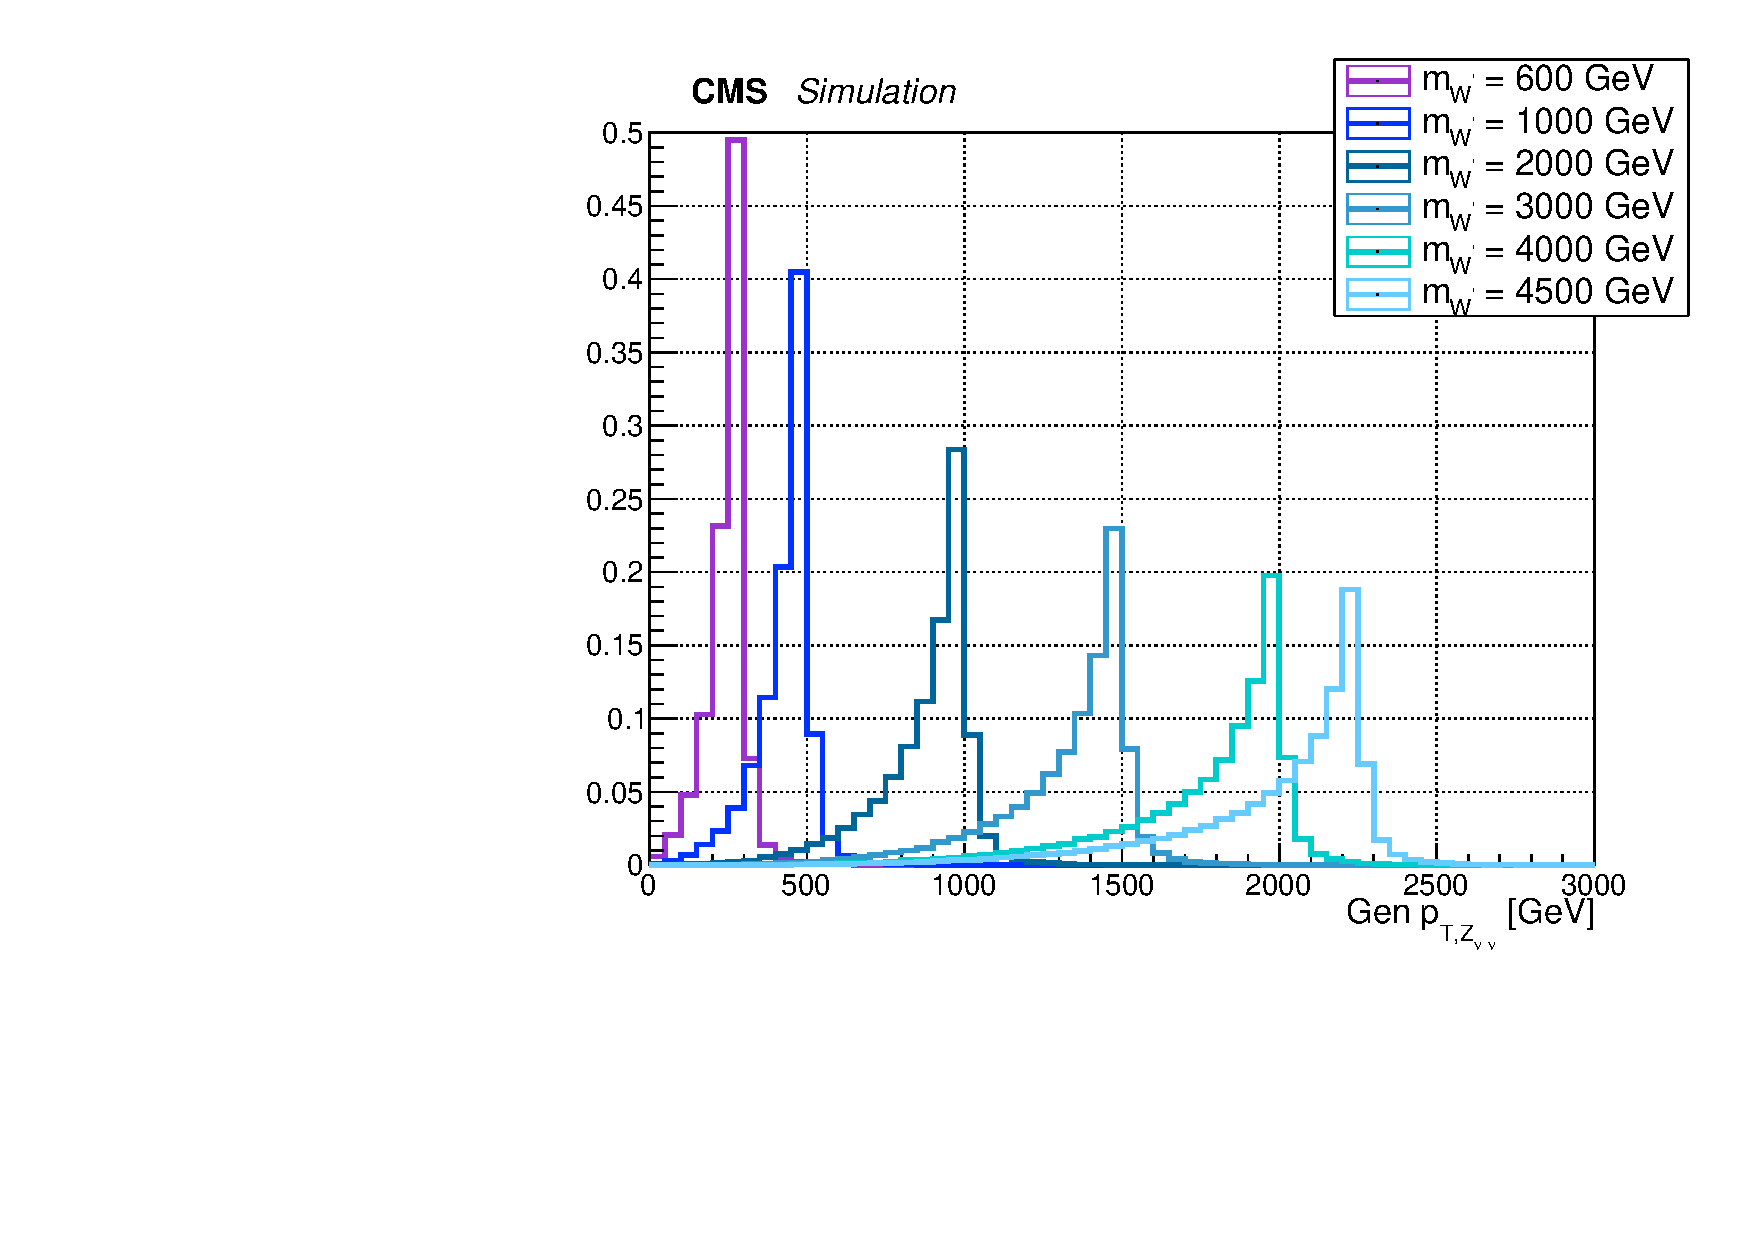
\includegraphics[width=.495\textwidth]{Gen_v9/XWZInv_g_ZLepPt.pdf}%GenHpt.pdf}
     \\
     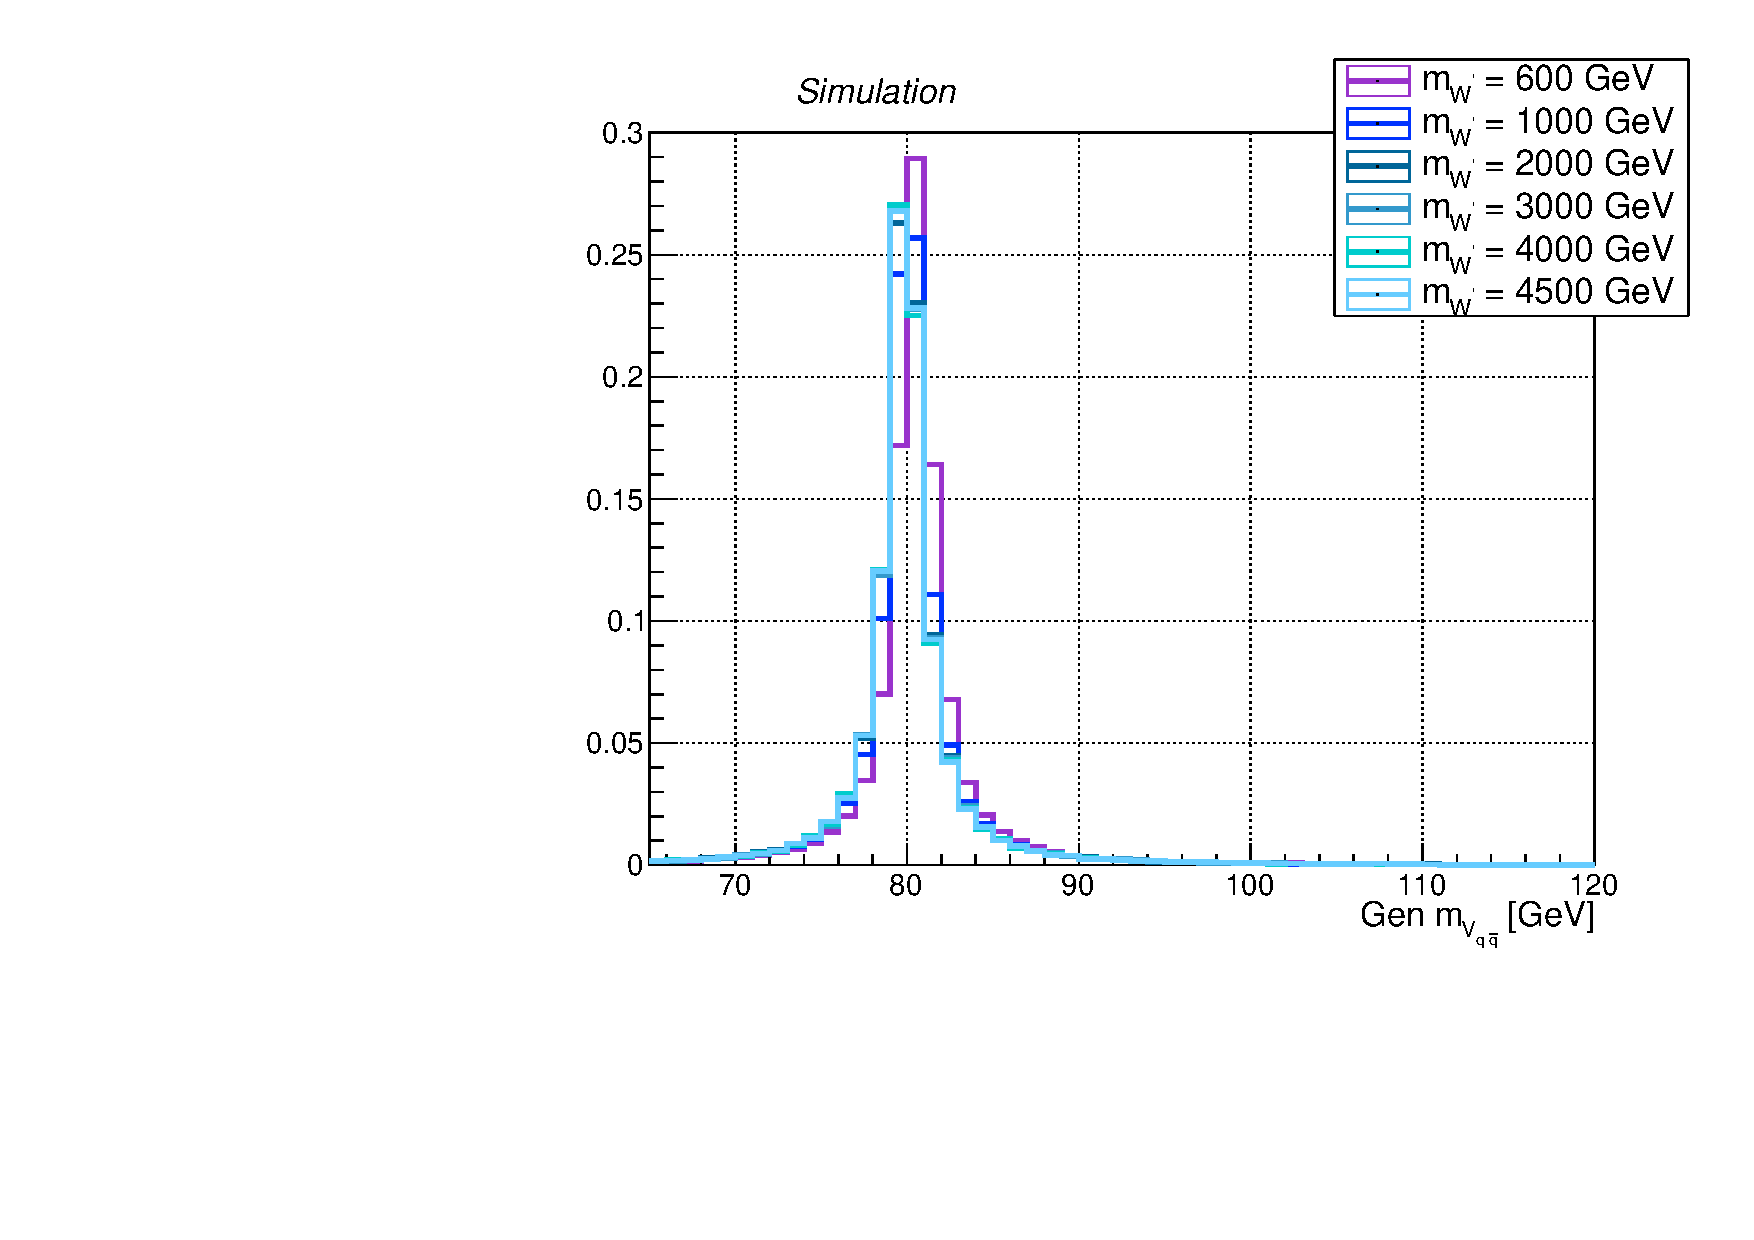
\includegraphics[width=.495\textwidth]{Gen_v9/XWZInv_g_VHadMass.pdf}%GenZdR.pdf}
     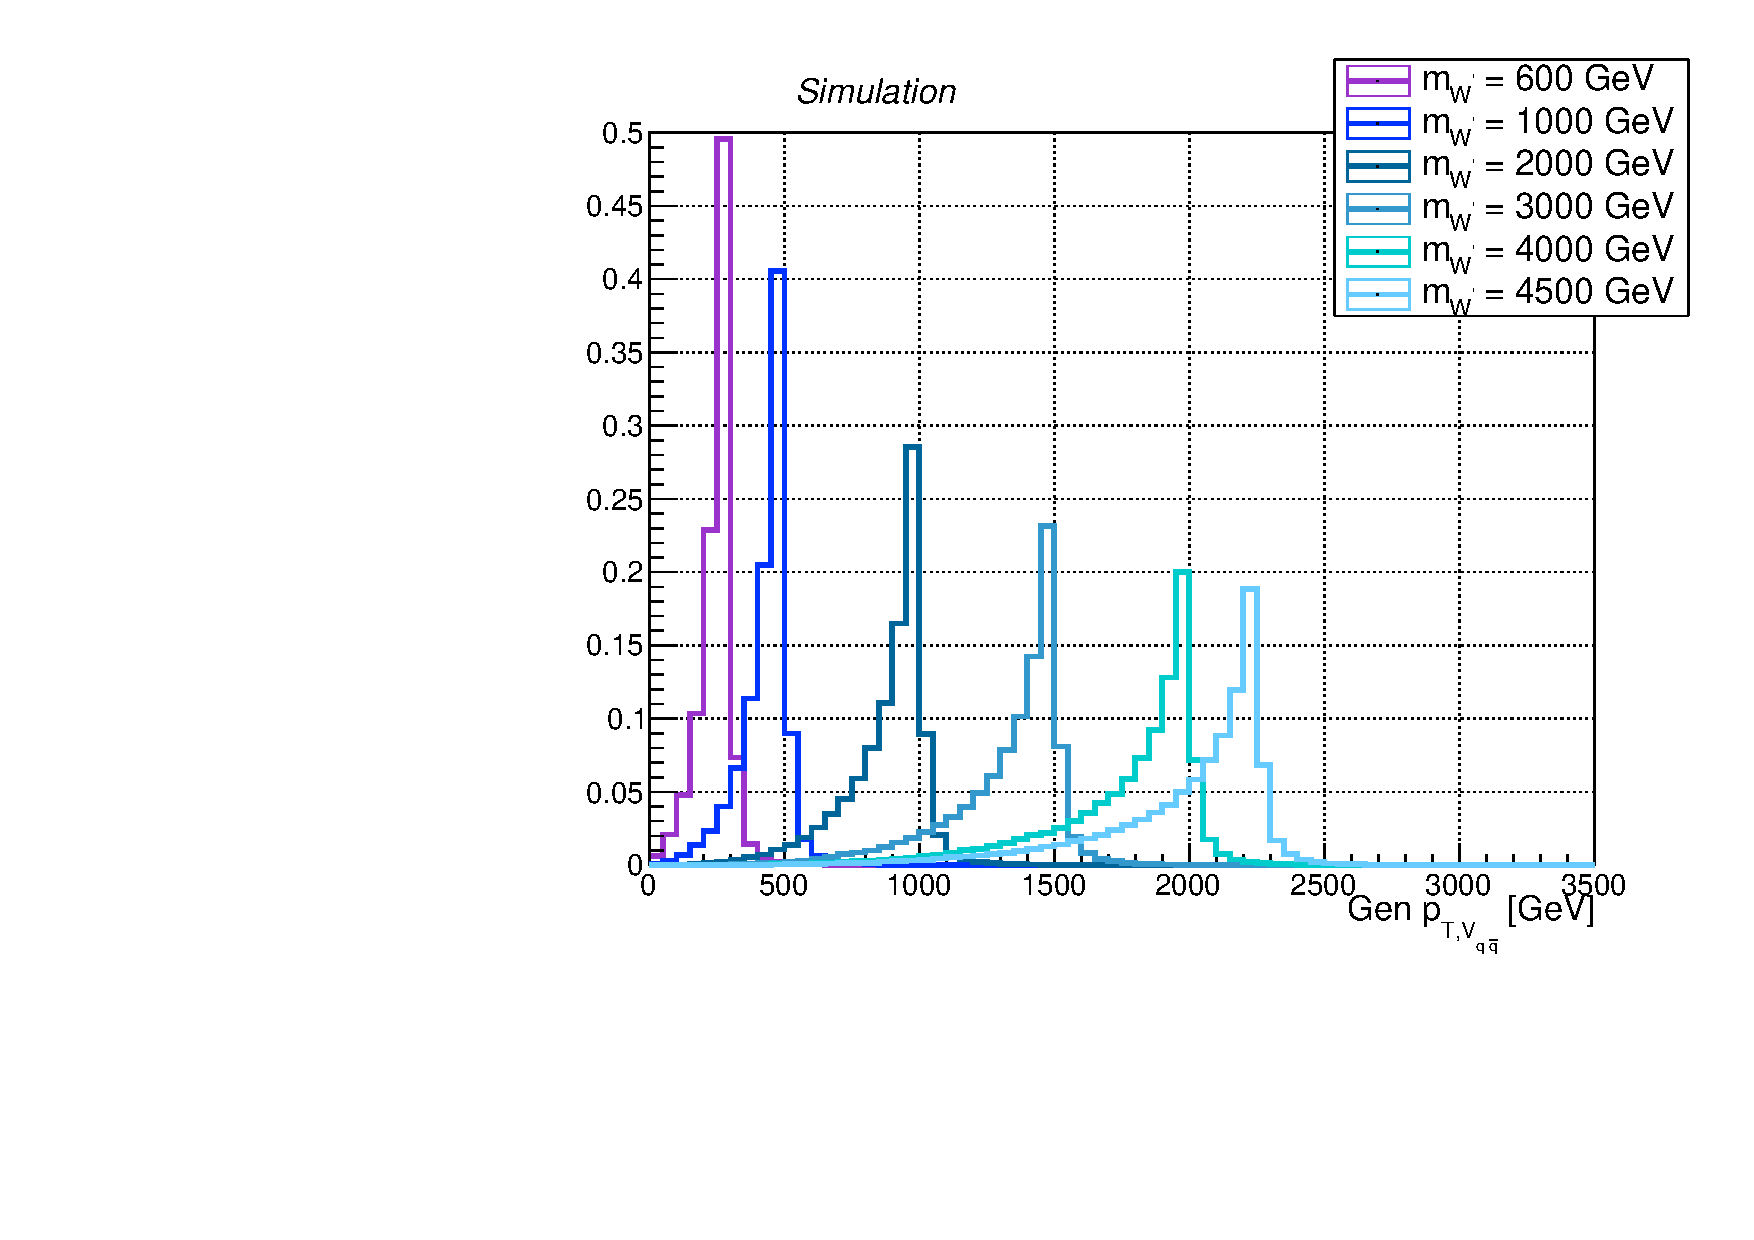
\includegraphics[width=.495\textwidth]{Gen_v9/XWZInv_g_VHadPt.pdf}%GenHdR.pdf}
   \end{center}
   \caption{Main signal kinematic quantities at generation level after parton showering, for spin-1 \Wp signal, considering different mass hypoteses ($m_{\Wp} = 0.6, 1, 2, 3, 4, 4.5$ TeV). Top: \Wp transverse mass and \pt distributions. Center: invisibly decaying \Z mass and \pt. Bottom: hadronically decaying \W mass and \pt.}
   \label{fig:genWprimeSignal1}
 \end{figure}

 \begin{figure}[!htb]
   \begin{center}
     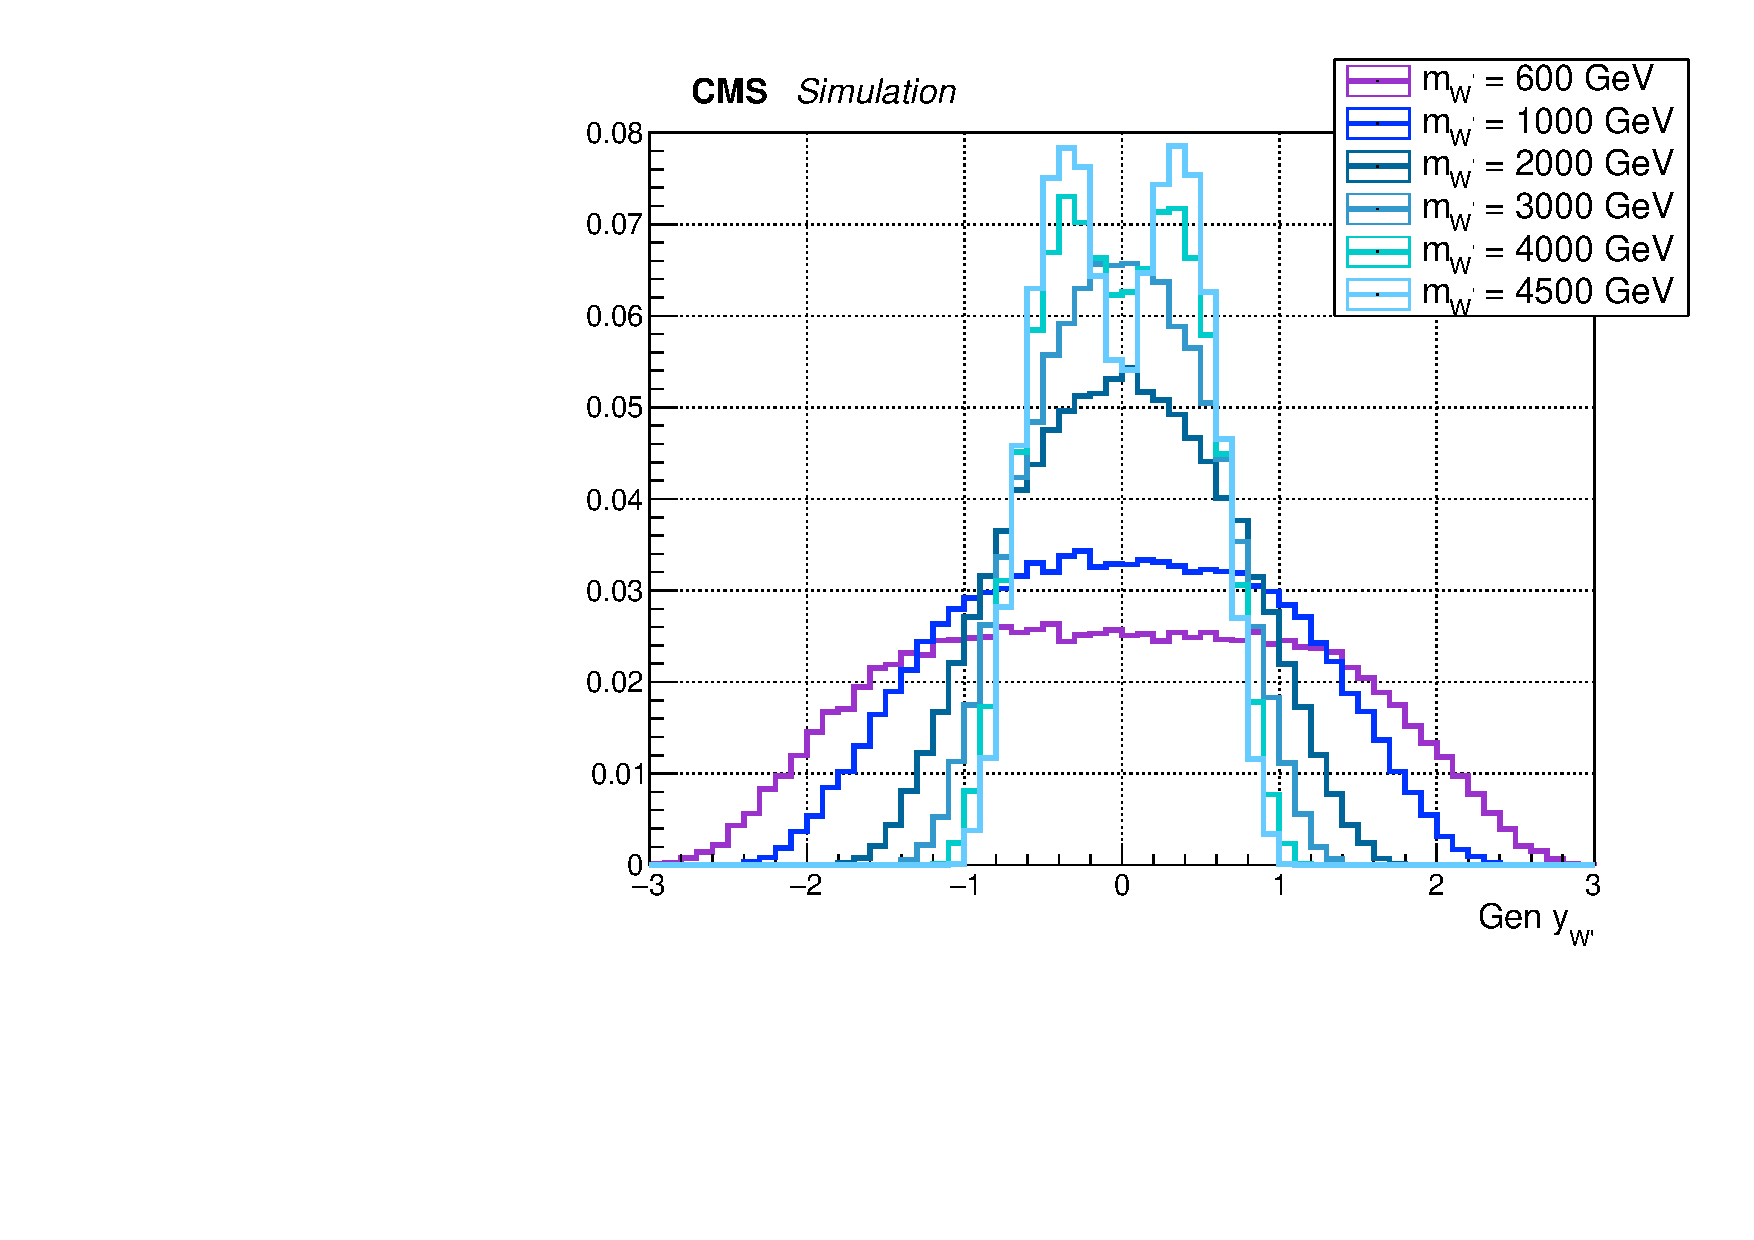
\includegraphics[width=.495\textwidth]{Gen_v9/XWZInv_g_XRapidity.pdf}%GenPhi1pt.pdf}
     %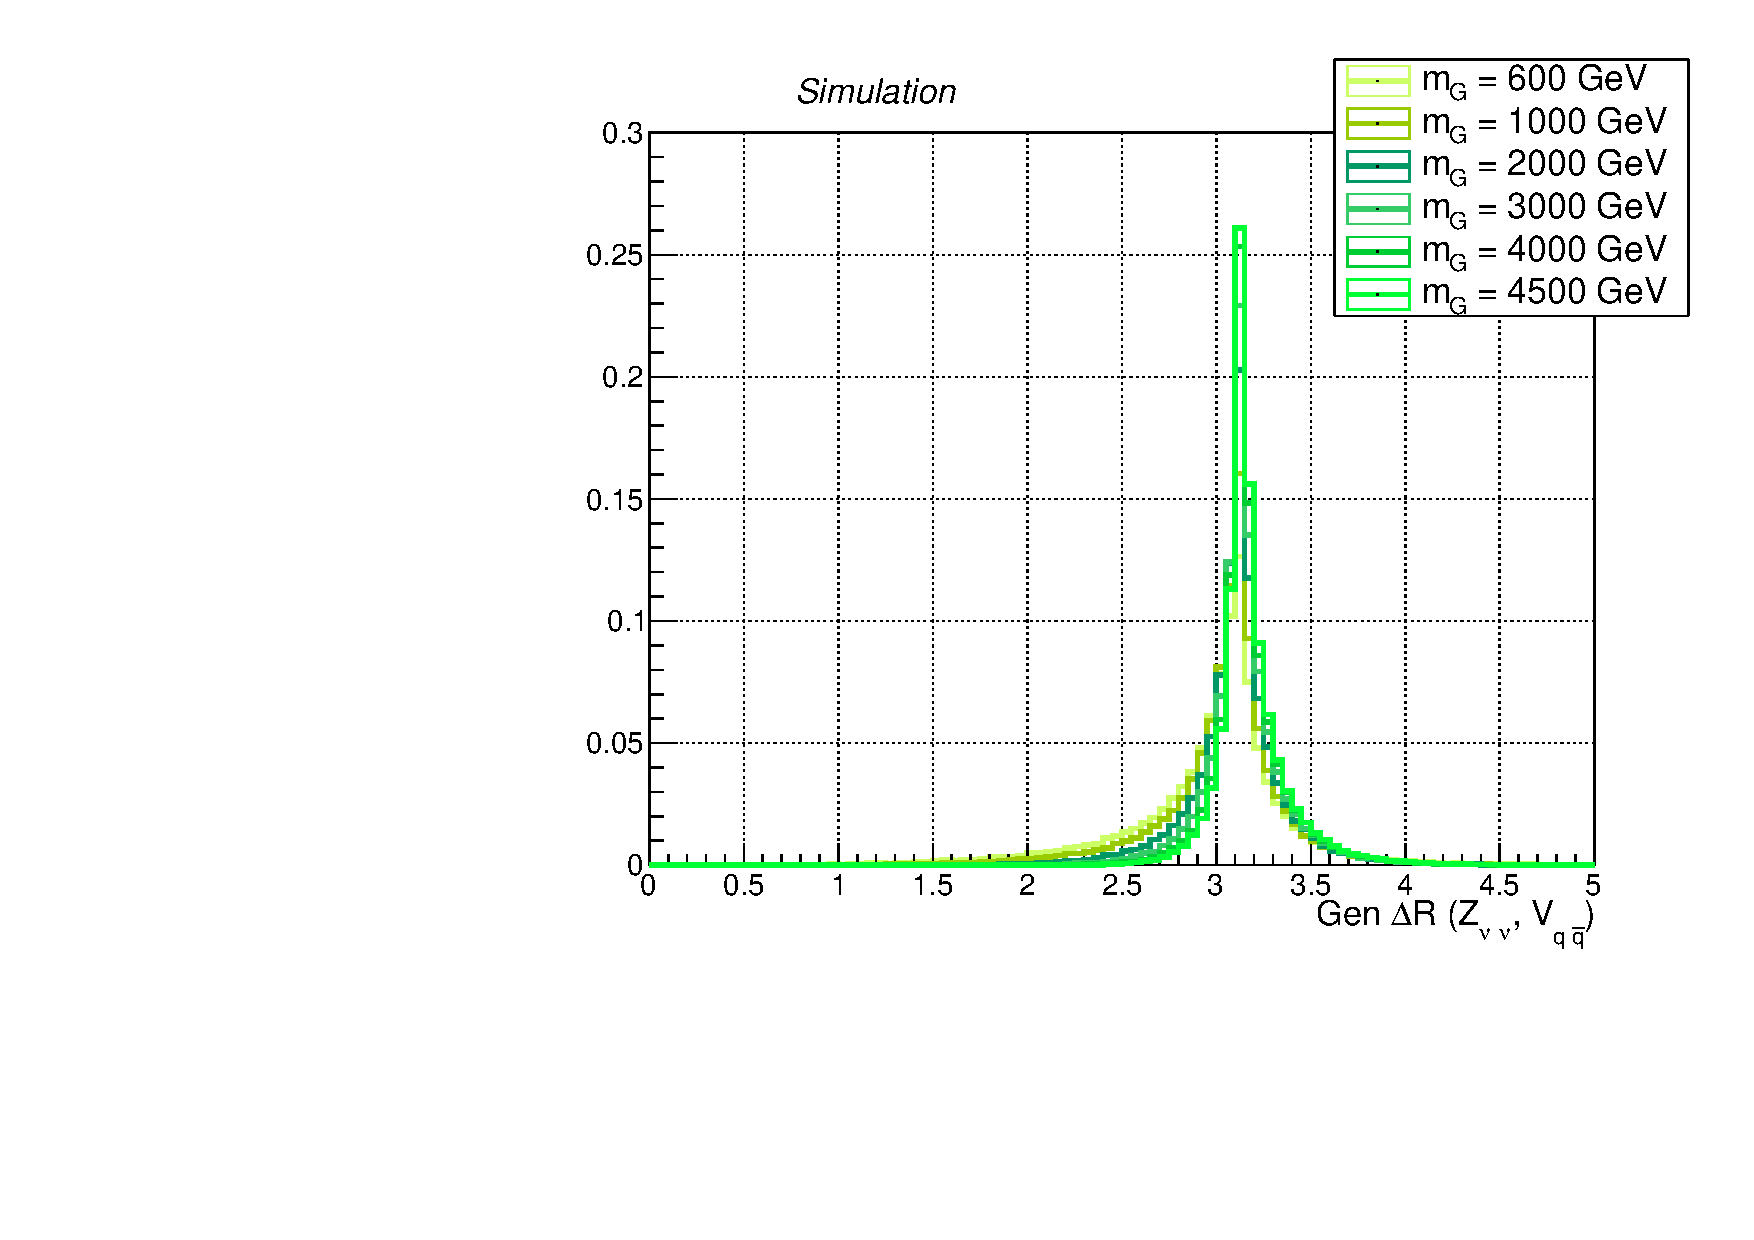
\includegraphics[width=.495\textwidth]{Gen_v9/XZZInv_g_VZDR.pdf}%GenPhi1y.pdf}
     %\\
     %\includegraphics[width=.495\textwidth]{Gen_v7/g_ZLepMass.pdf}%GenZmass.pdf}
     %\includegraphics[width=.495\textwidth]{Gen_v7/g_ZHadMass.pdf}%GenHmass.pdf}
     \\
     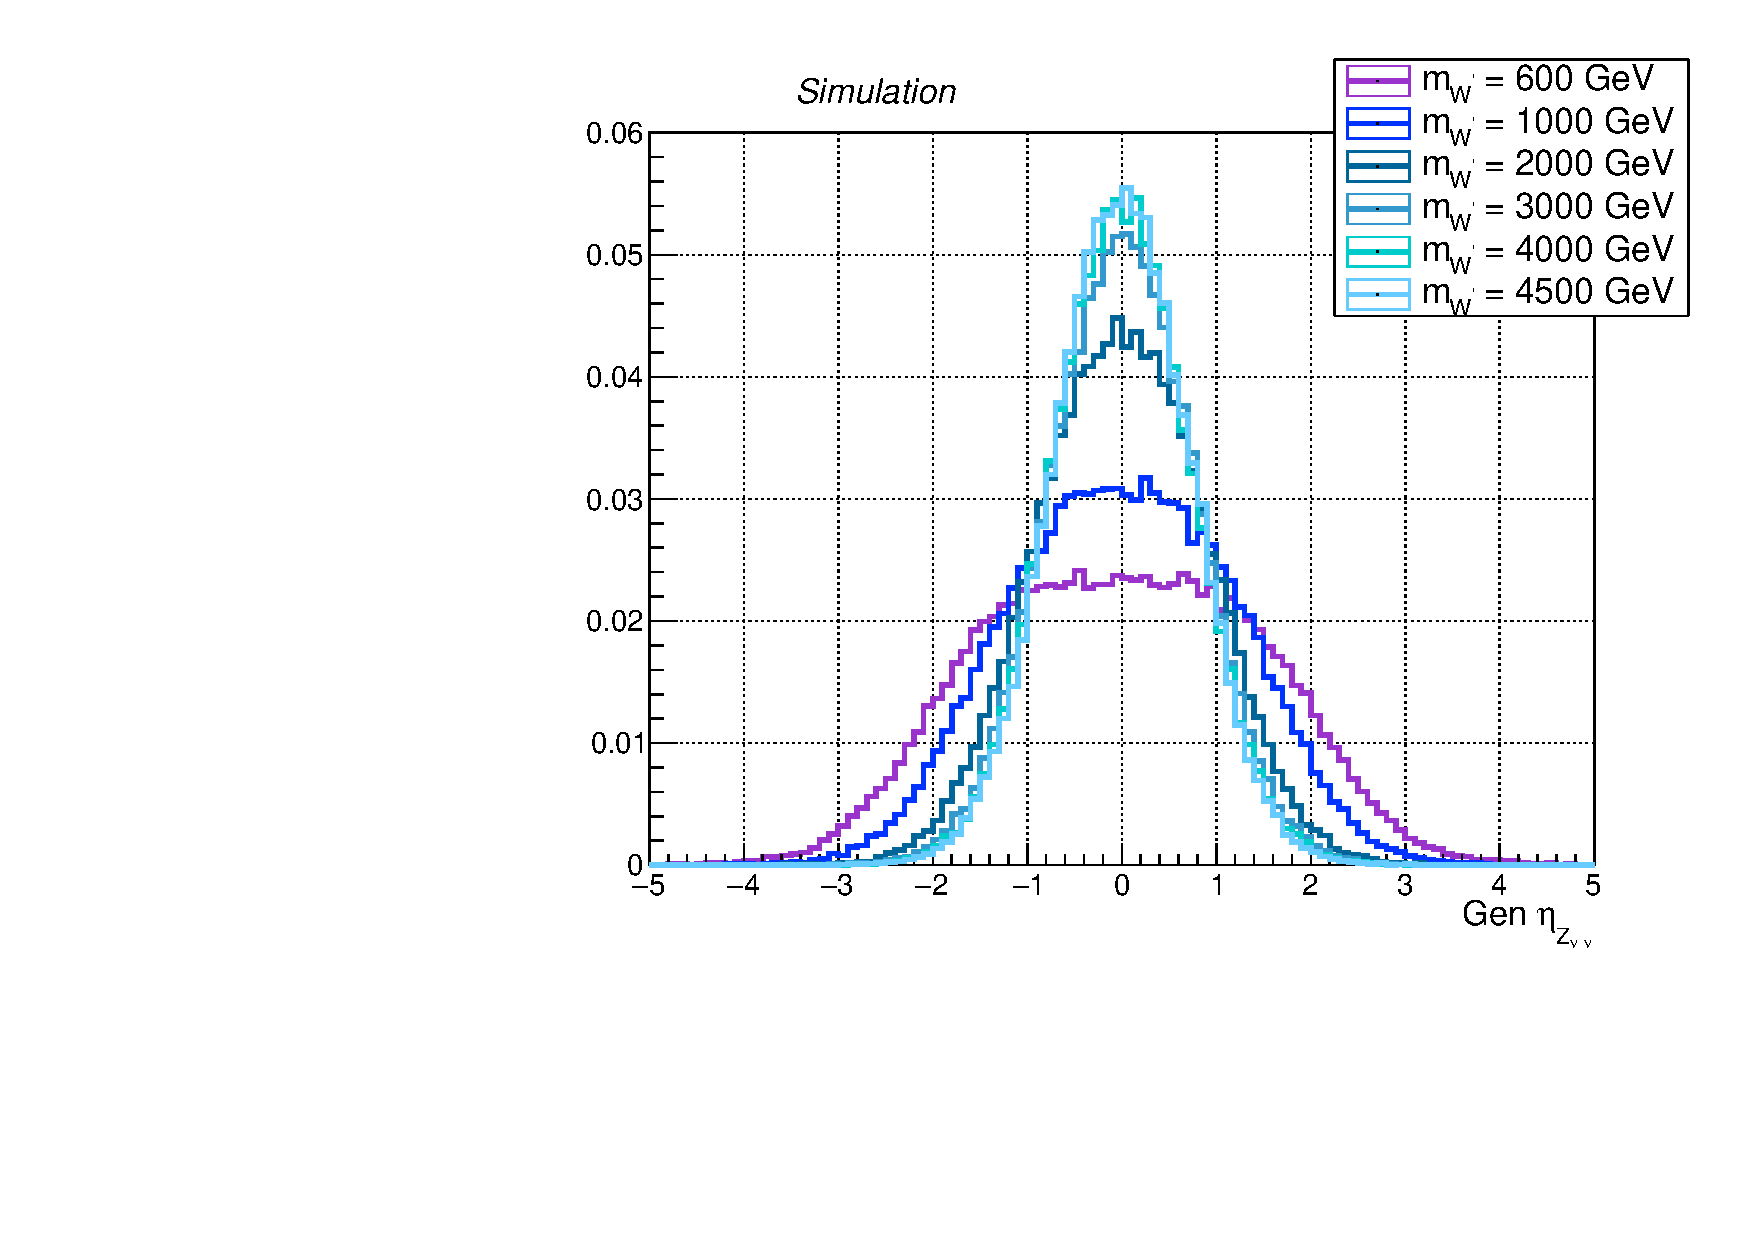
\includegraphics[width=.495\textwidth]{Gen_v9/XWZInv_g_ZLepEta.pdf}%GenZpt.pdf}
     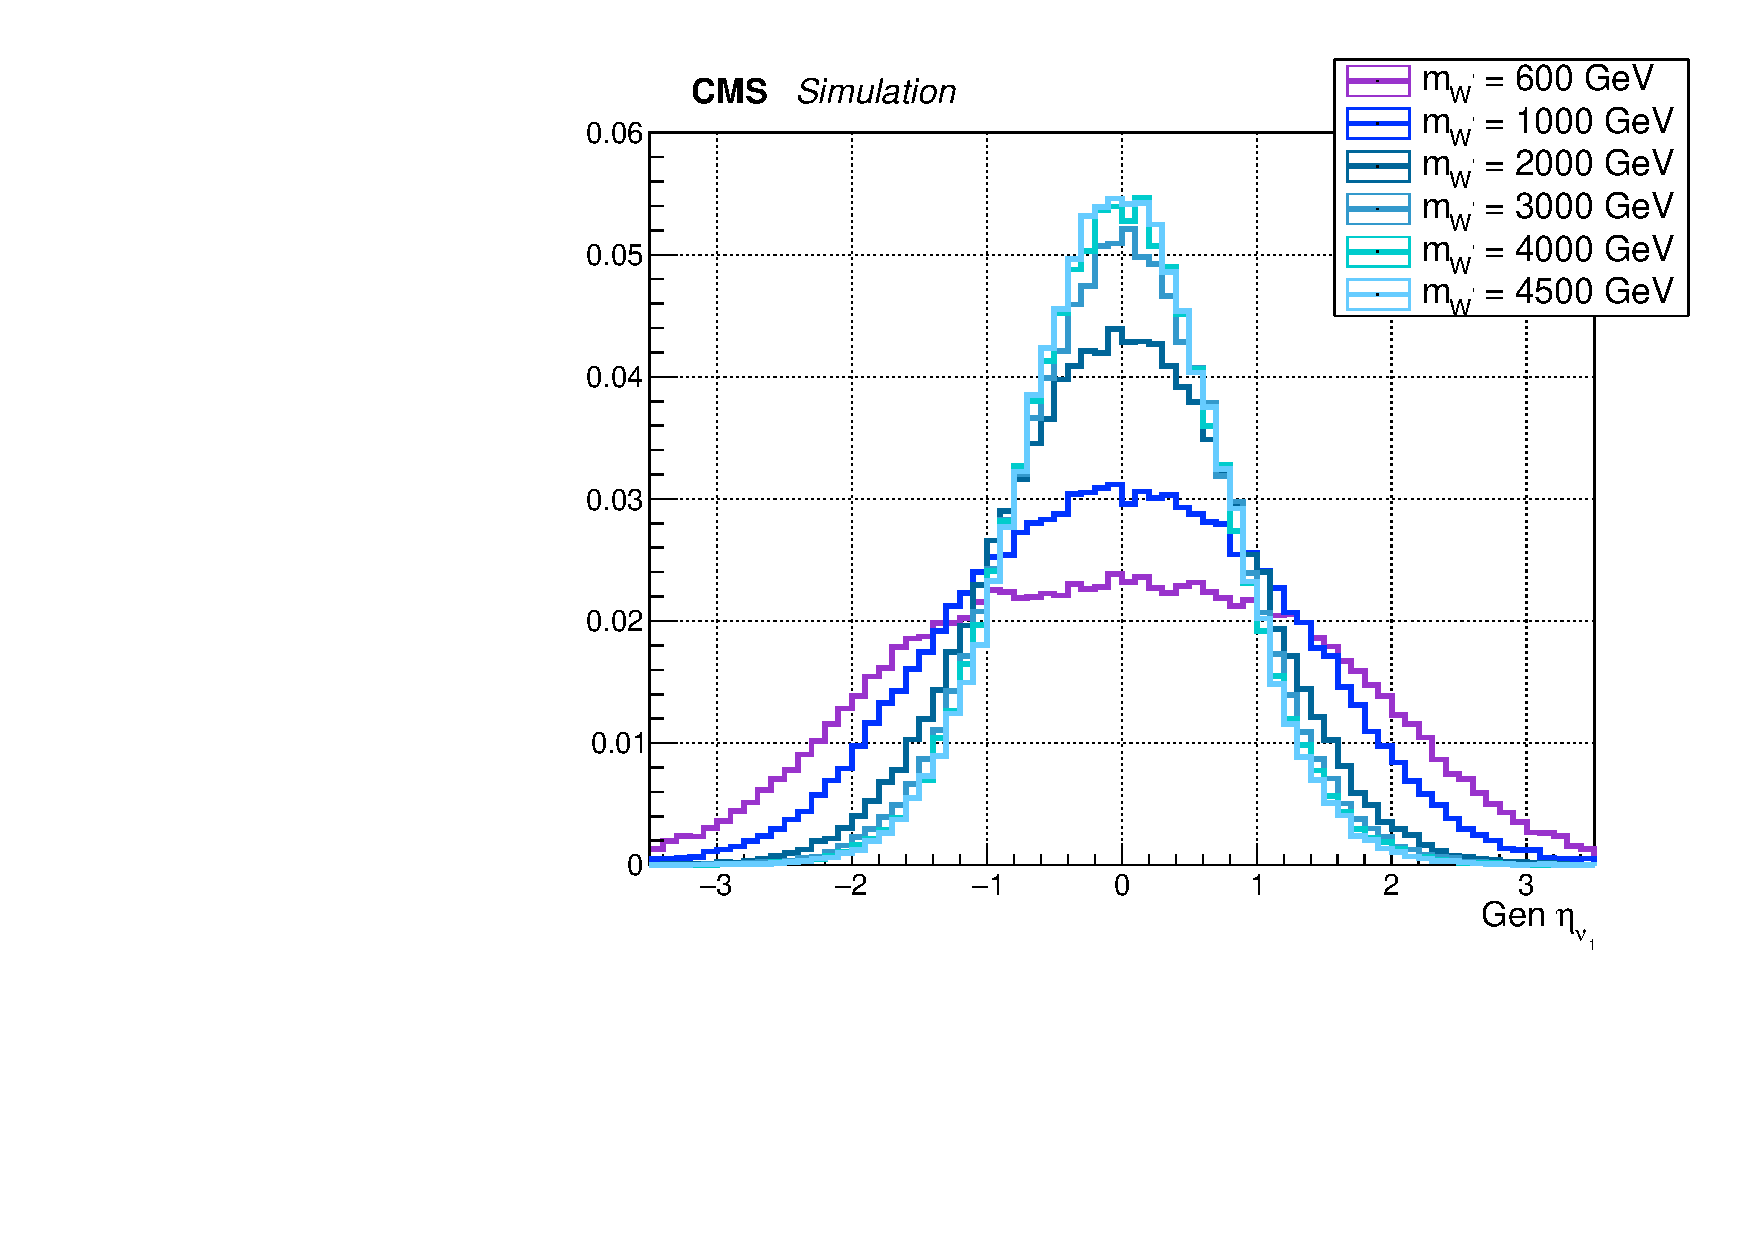
\includegraphics[width=.495\textwidth]{Gen_v9/XWZInv_g_Lep1Eta.pdf}%GenHpt.pdf}
     \\
     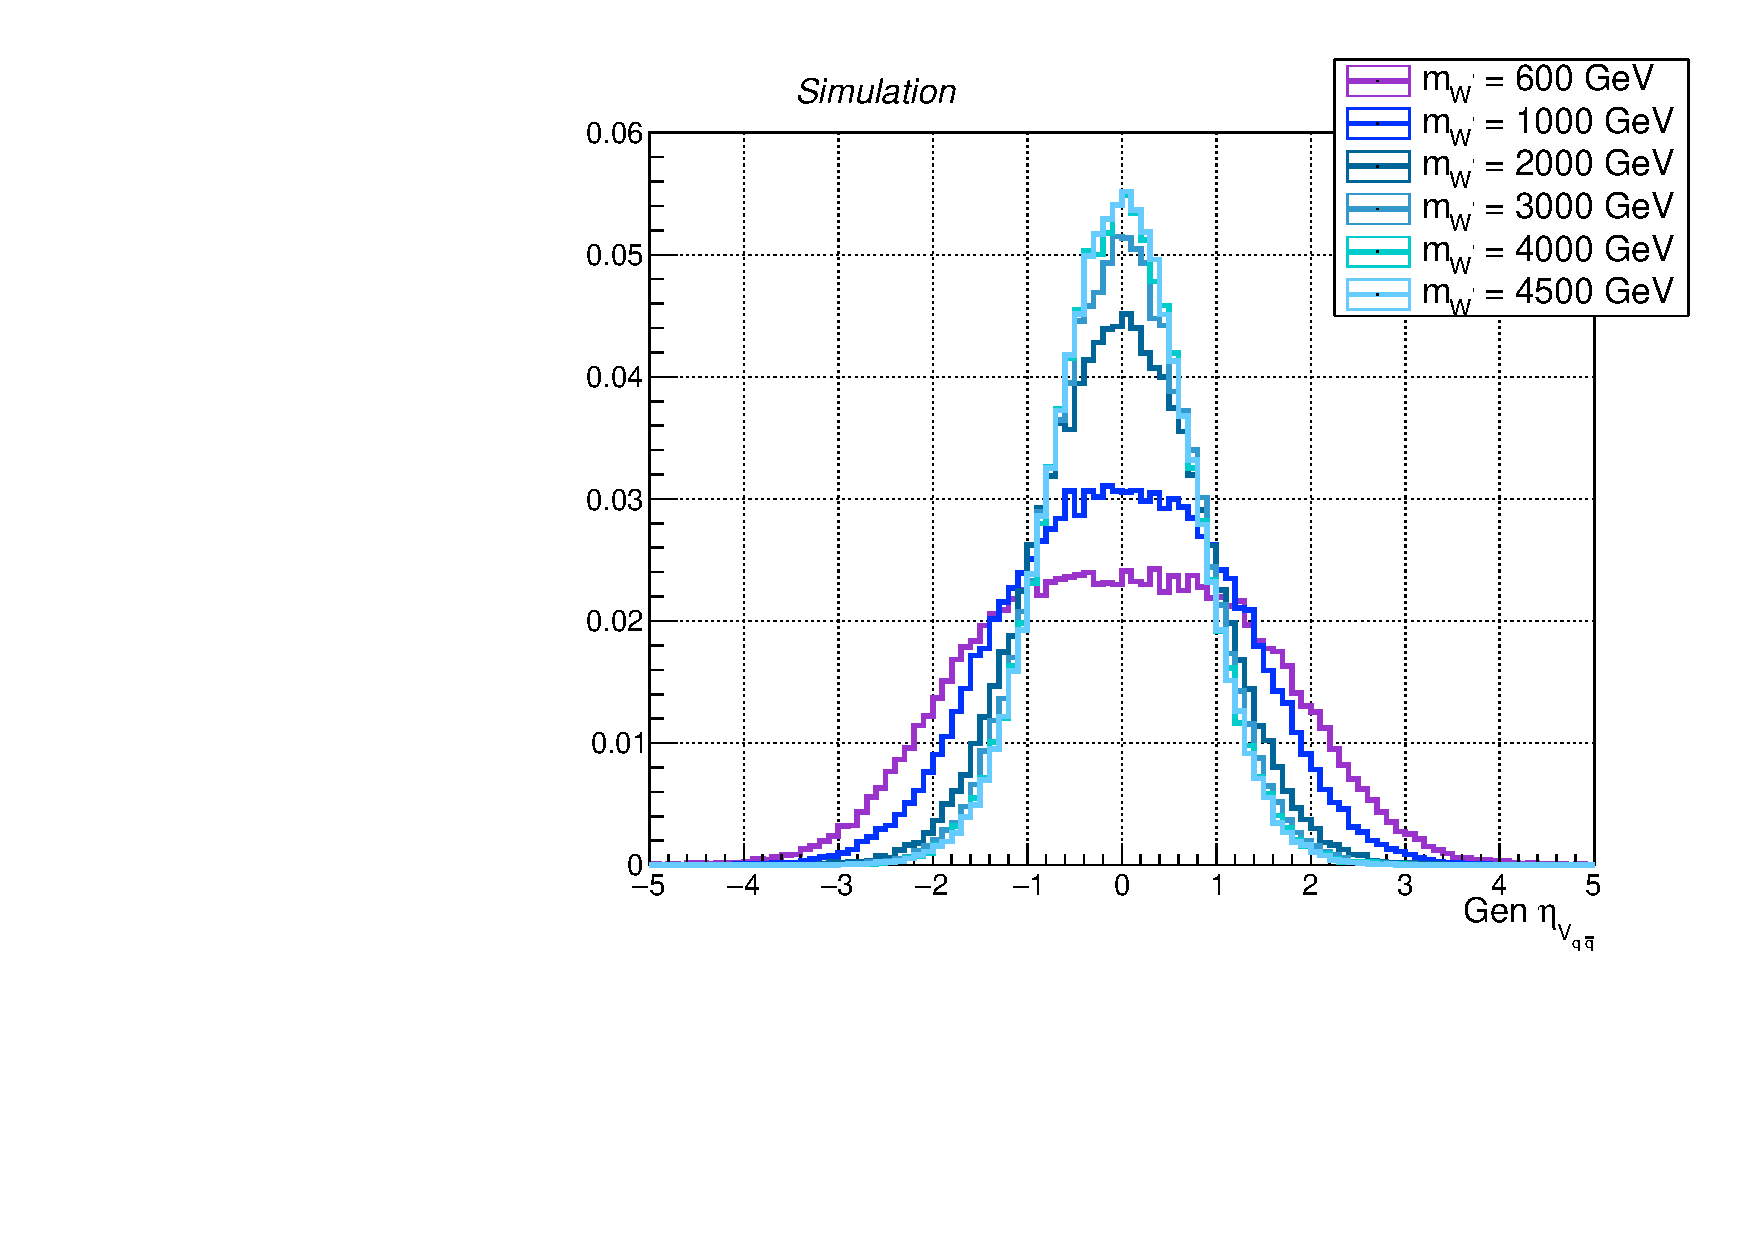
\includegraphics[width=.495\textwidth]{Gen_v9/XWZInv_g_VHadEta.pdf}%GenZdR.pdf}
     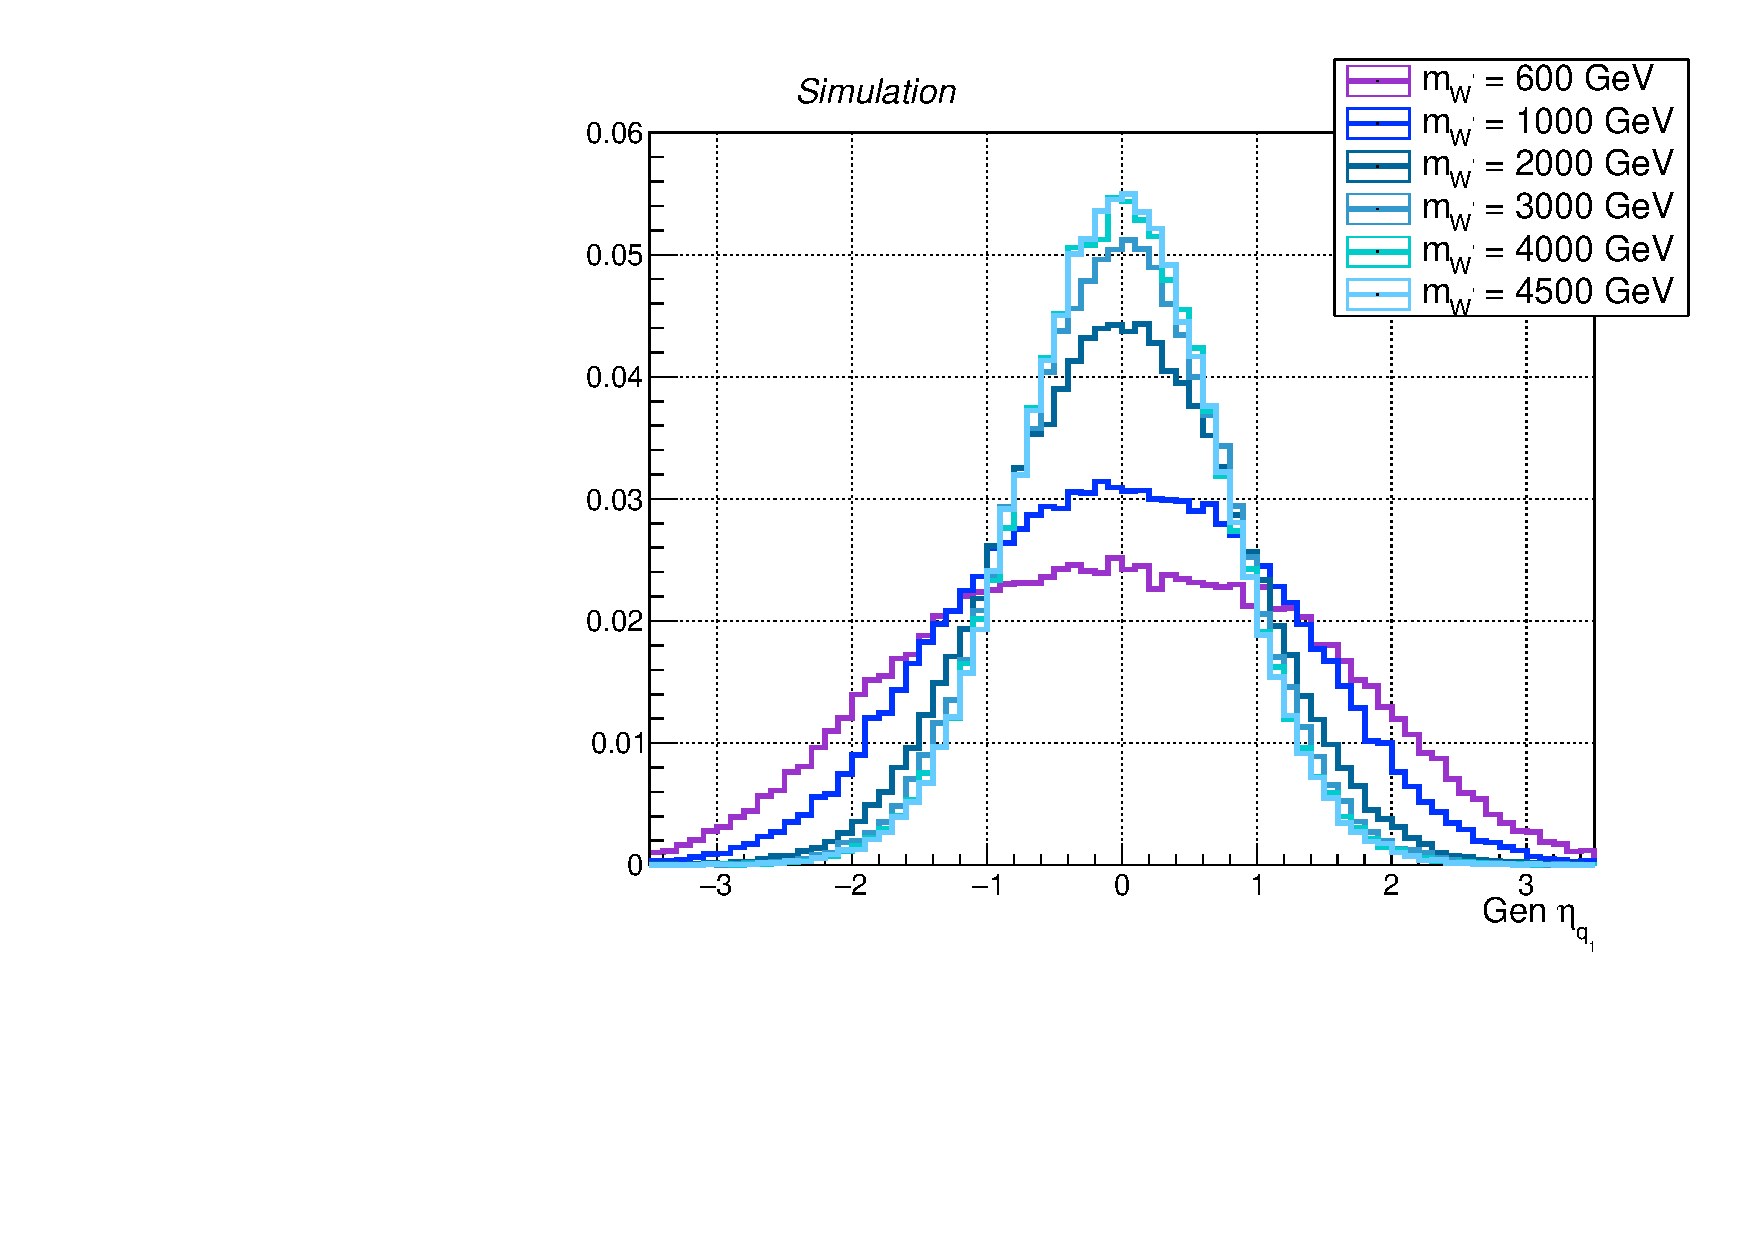
\includegraphics[width=.495\textwidth]{Gen_v9/XWZInv_g_Had1Eta.pdf}%GenHdR.pdf}
   \end{center}
   \caption{Main signal kinematic quantities at generation level after parton showering, for spin-1 \Wp signal, considering different mass hypoteses ($m_{\Wp} = 0.6, 1, 2, 3, 4, 4.5$ TeV). Top: \Wp rapidity $\mathcal{Y}$. Center: pseudorapidity $\eta$ of the invisibly decaying \Z, and pseudorapidity of the leading neutrino. Bottom: pseudorapidity $\eta$ of the hadronically decaying \W, and pseudorapidity of the leading quark.}
   \label{fig:genWprimeSignal2}
 \end{figure}

 \begin{figure}[!htb]
   \begin{center}
     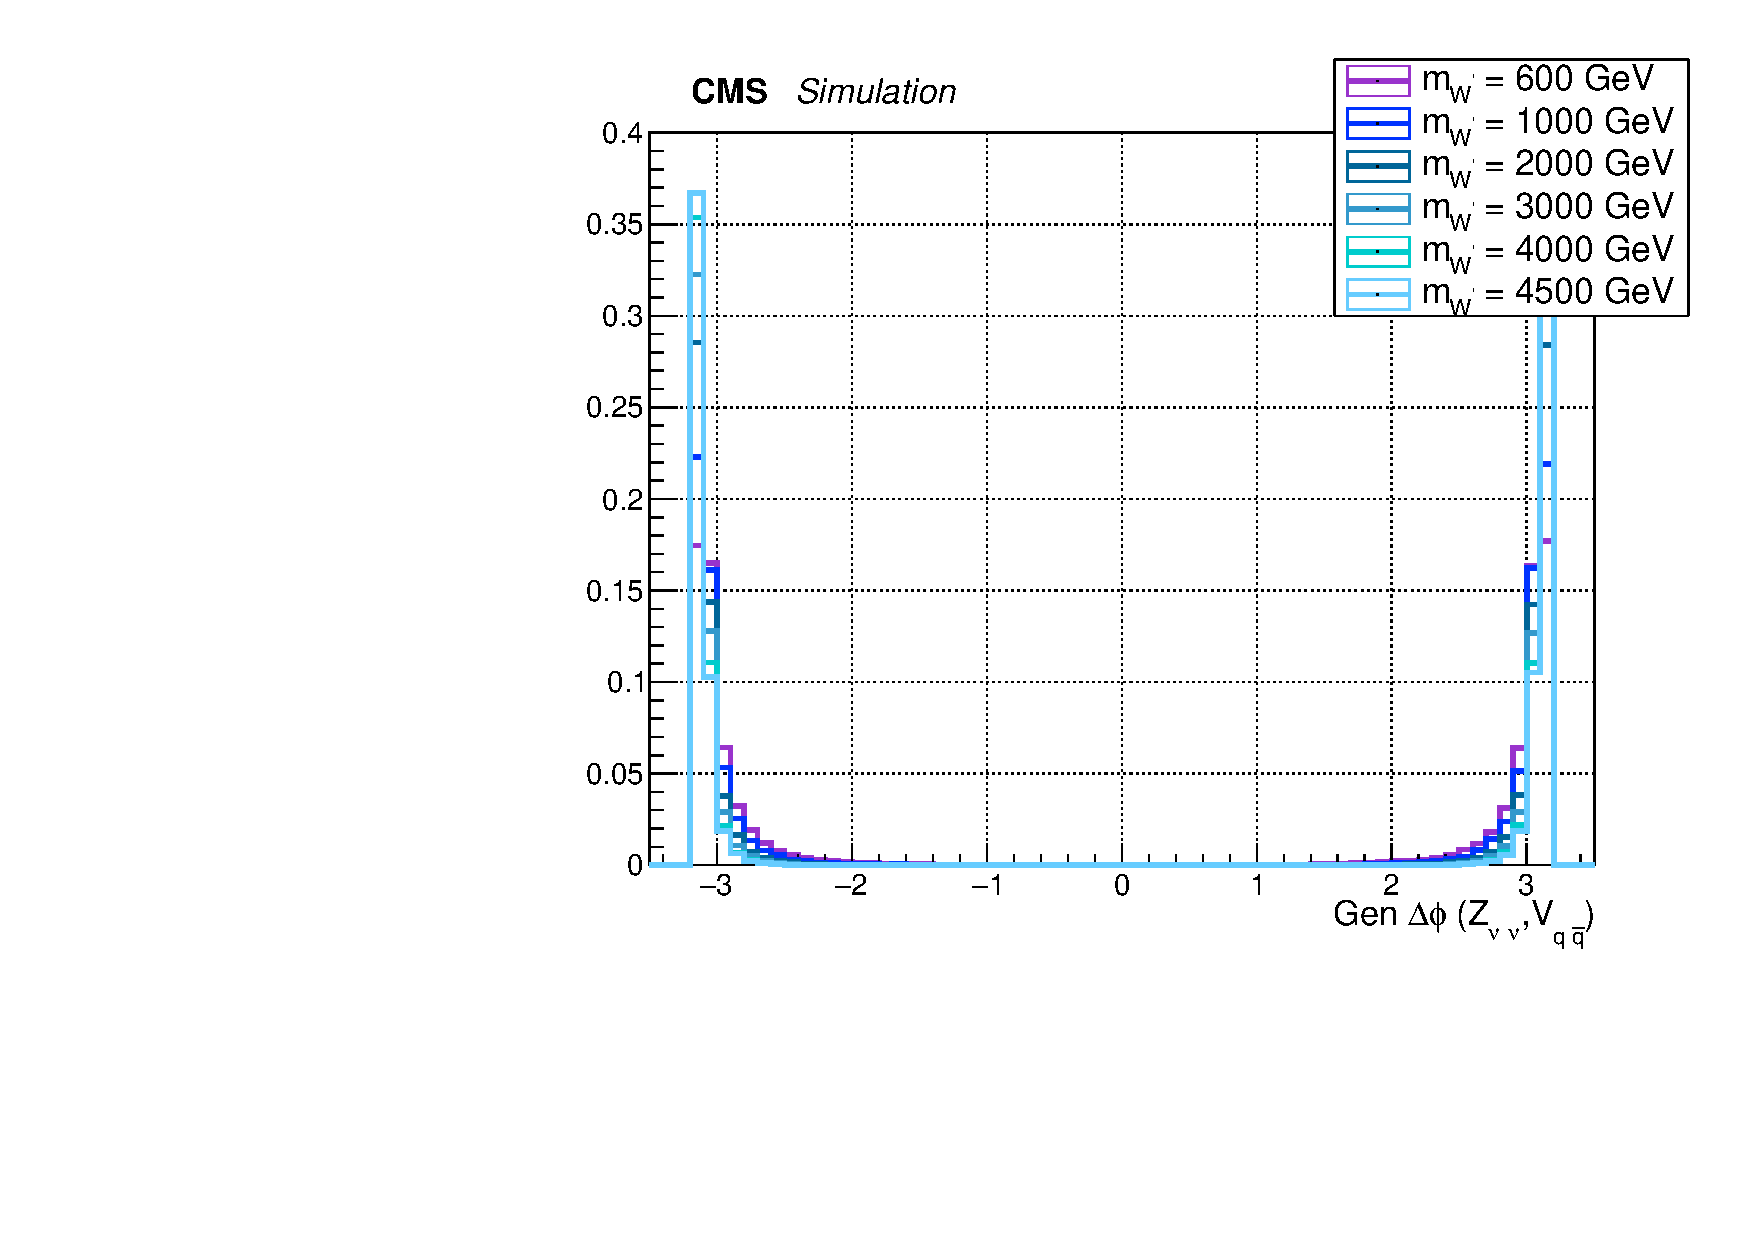
\includegraphics[width=.495\textwidth]{Gen_v9/XWZInv_g_VZDPhi.pdf}%GenPhi1pt.pdf}
     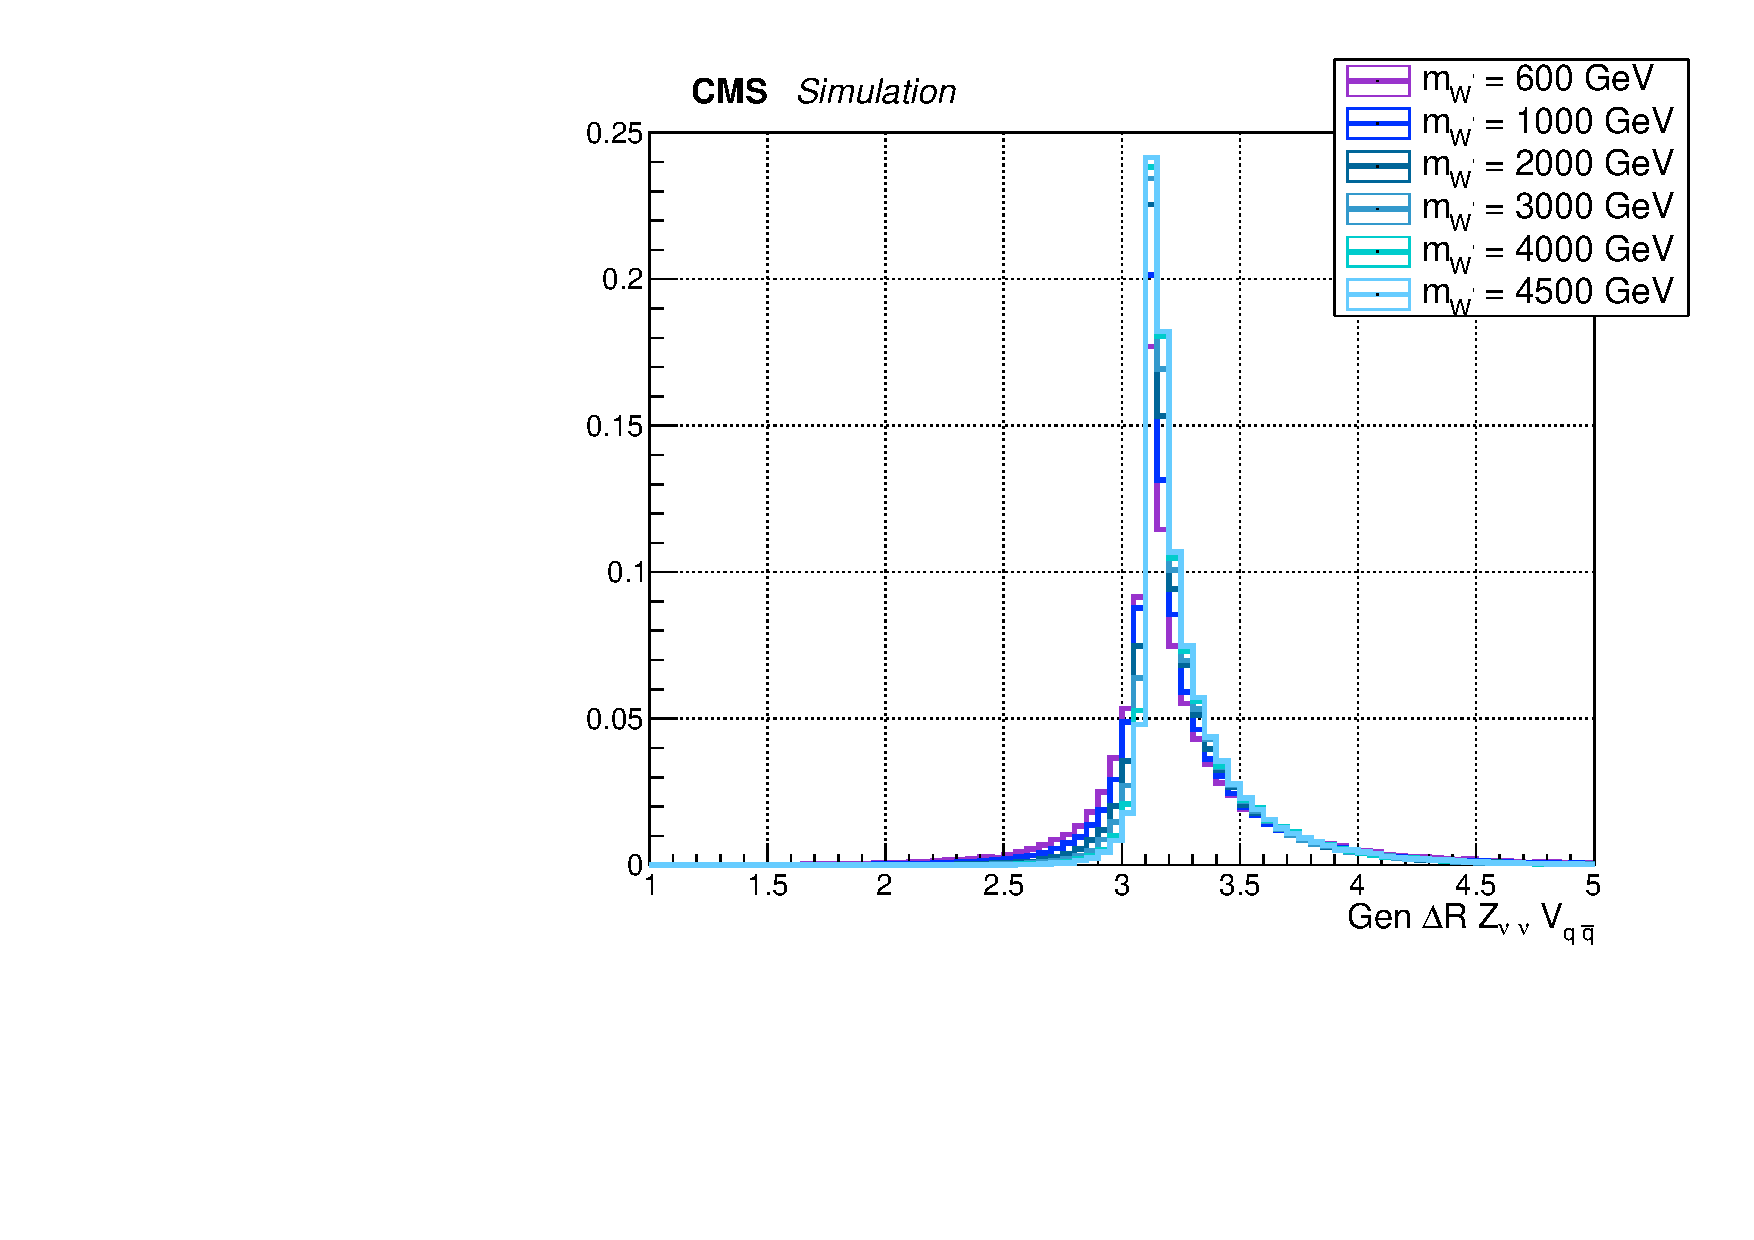
\includegraphics[width=.495\textwidth]{Gen_v9/XWZInv_g_VZDR.pdf}%GenPhi1y.pdf}
     %\\
     %\includegraphics[width=.495\textwidth]{Gen_v7/g_ZLepMass.pdf}%GenZmass.pdf}
     %\includegraphics[width=.495\textwidth]{Gen_v7/g_ZHadMass.pdf}%GenHmass.pdf}
     \\
     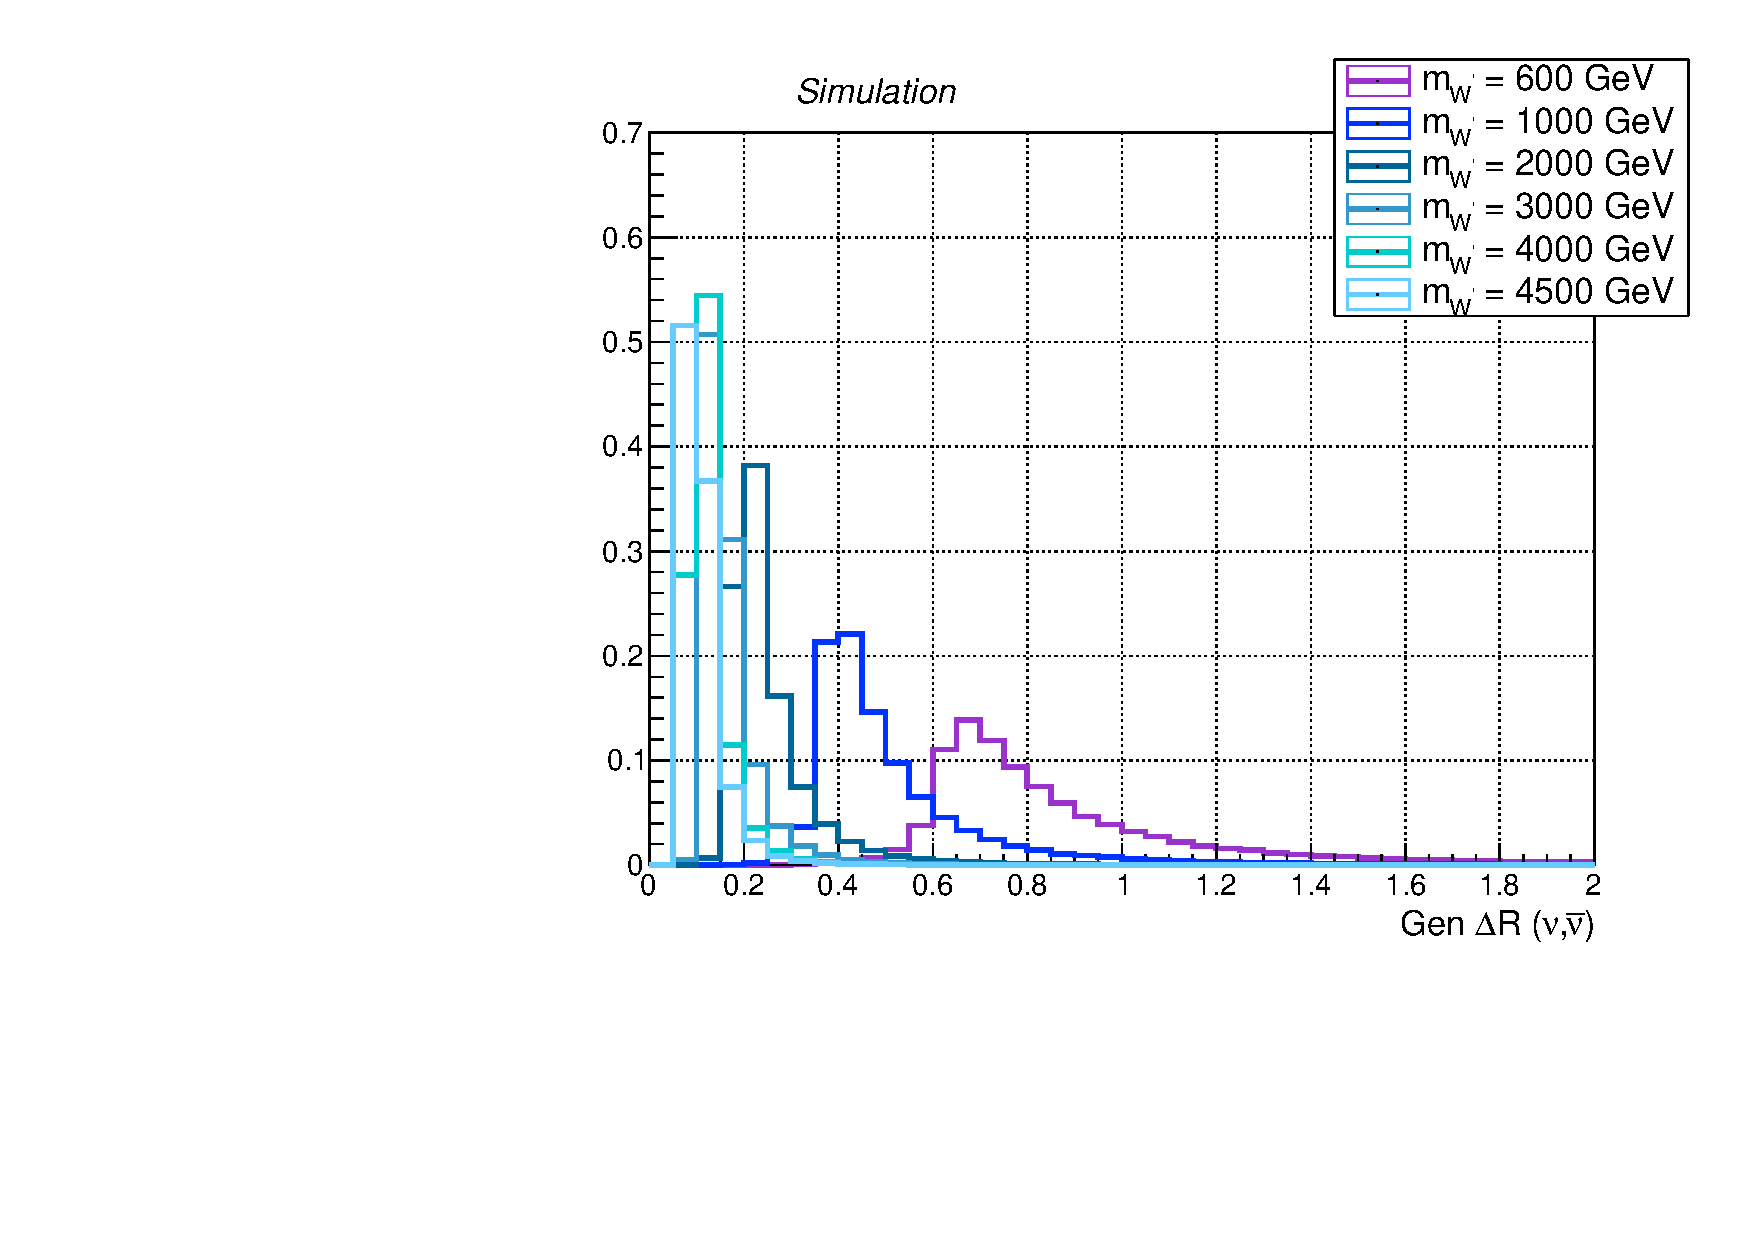
\includegraphics[width=.495\textwidth]{Gen_v9/XWZInv_g_LepDR.pdf}%GenZpt.pdf}
     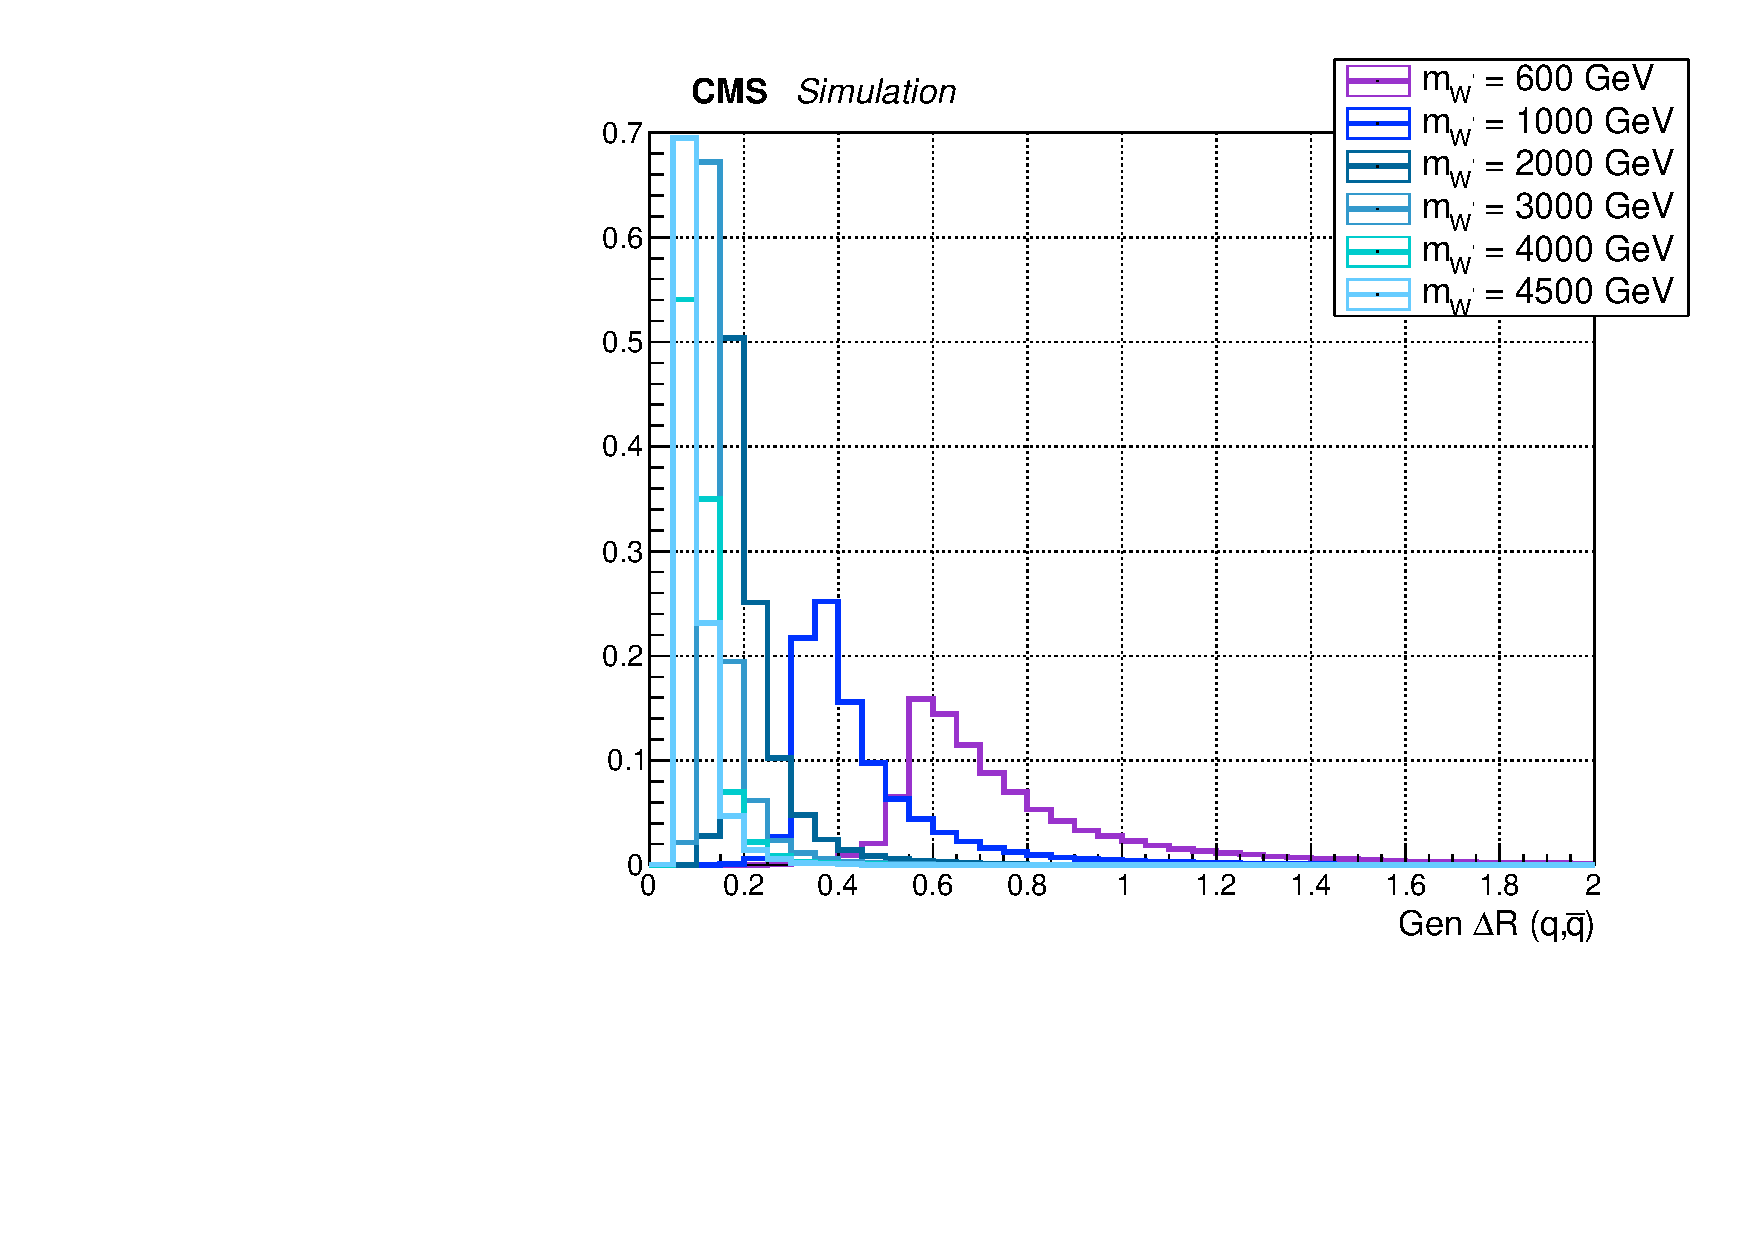
\includegraphics[width=.495\textwidth]{Gen_v9/XWZInv_g_HadDR.pdf}%GenHpt.pdf}
     \\
     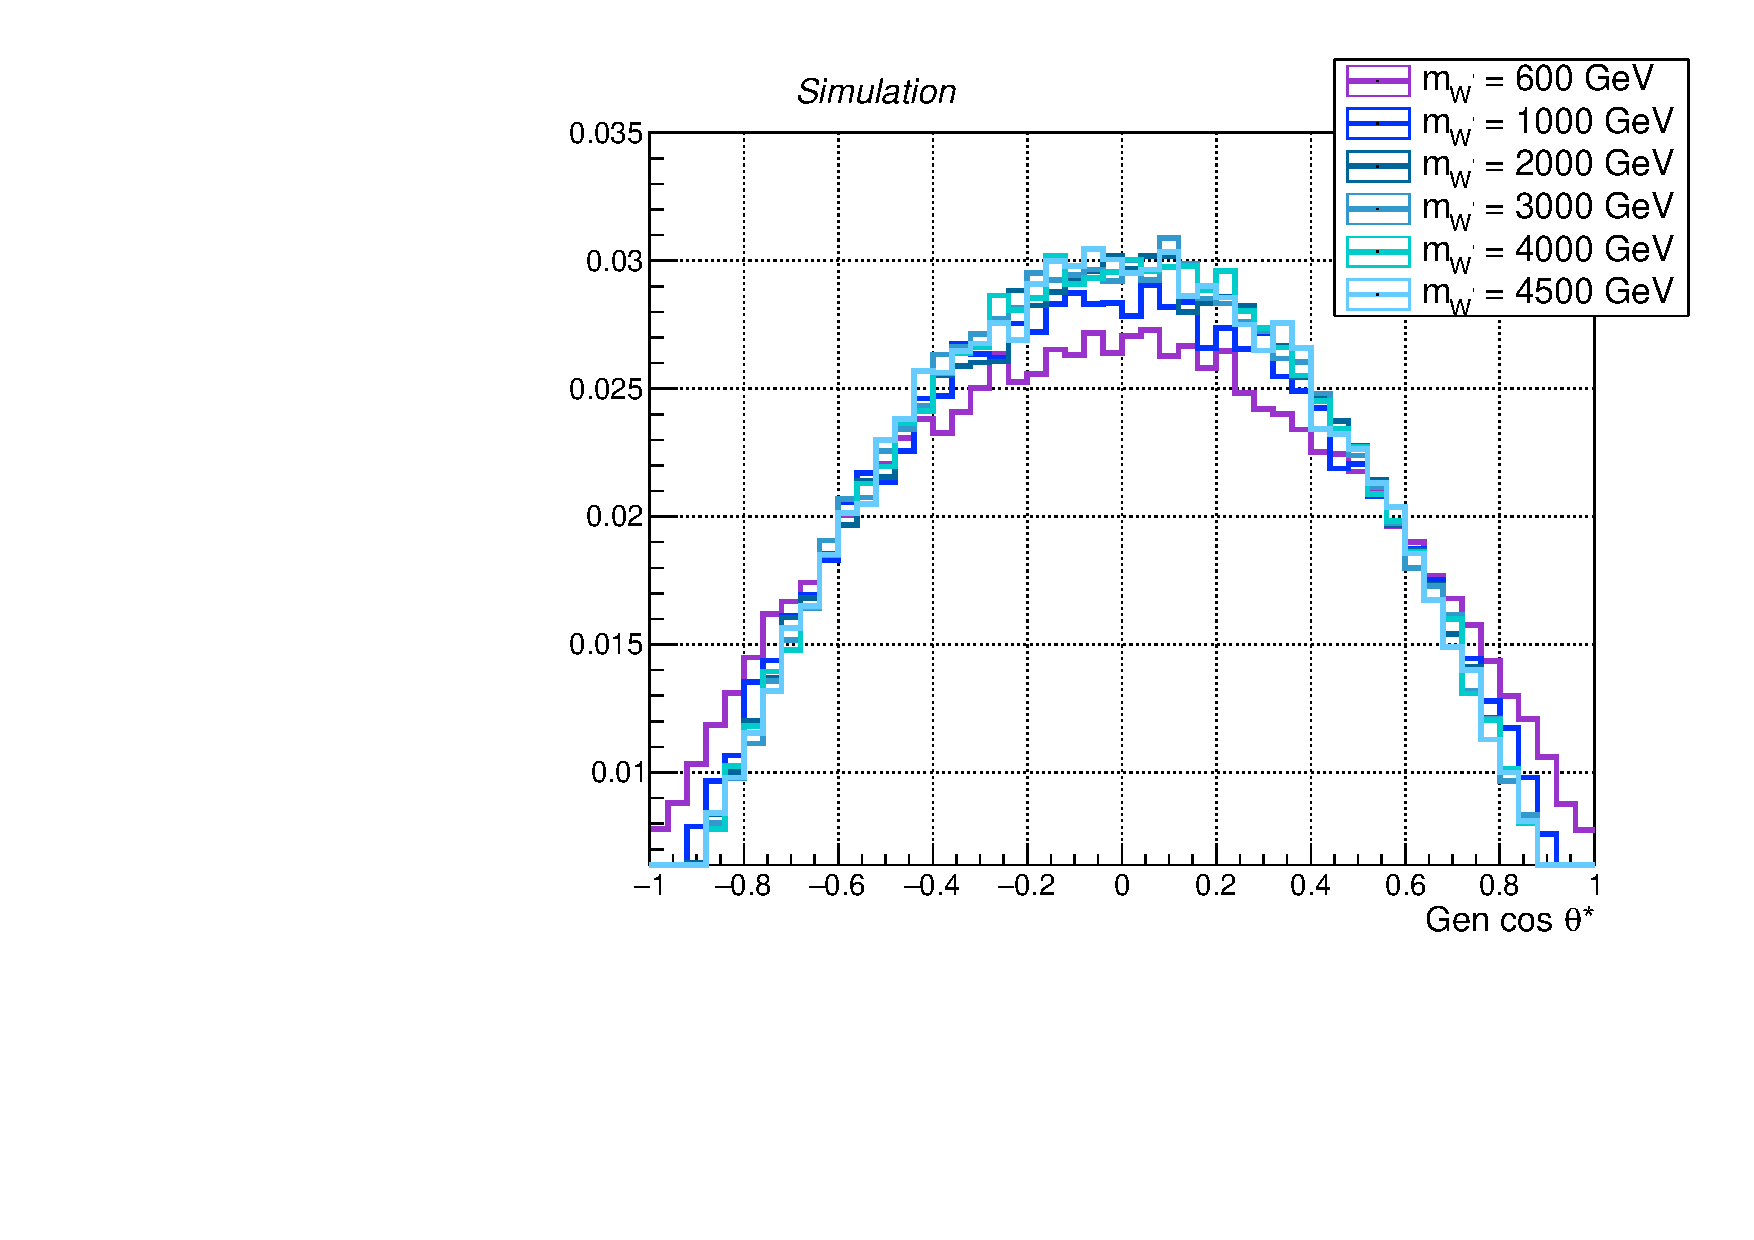
\includegraphics[width=.495\textwidth]{Gen_v9/XWZInv_g_CosThetaStar.pdf}%GenZdR.pdf}
     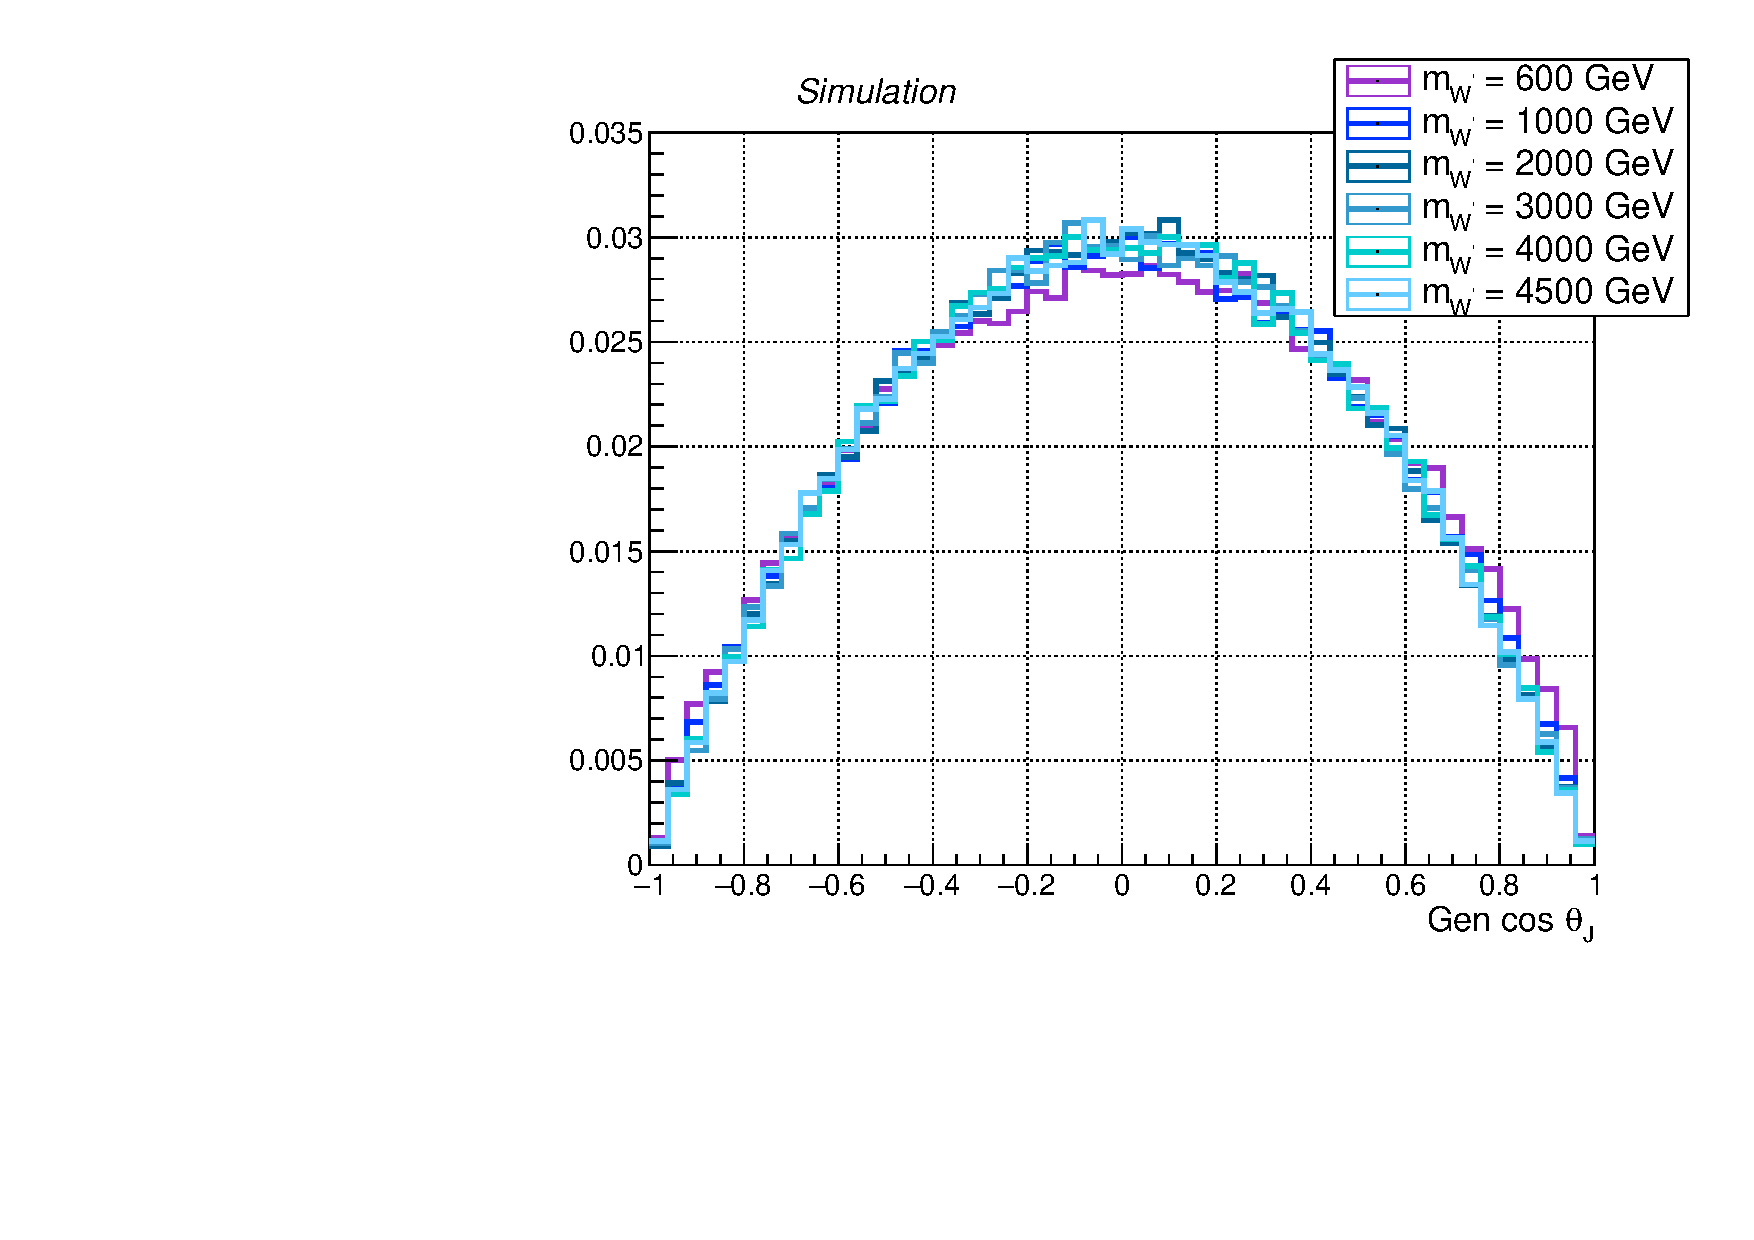
\includegraphics[width=.495\textwidth]{Gen_v9/XWZInv_g_CosThetaJ.pdf}%GenHdR.pdf}
   \end{center}
   \caption{Main signal kinematic quantities at generation level after parton showering, for spin-1 \Wp signal, considering different mass hypoteses ($m_{\Wp} = 0.6, 1, 2, 3, 4, 4.5$ TeV). Top: angular separation in the transverse plane $\Delta \phi$ (left) and solid angle $\Delta R$ (right) between leptonic \Z and hadronic \W. Center: solid angle between the neutrinos and the quarks. Bottom: distribution of $\cos{\theta}^{*}$ and $\cos{\theta}_{J}$ (described in text).}
   \label{fig:genWprimeSignal3}
 \end{figure}

\clearpage

\noindent Angular distributions are related to the spin, the polarization and the kinematics of the produced resonance; in particular:
\begin{itemize}
\item the $\Delta R$ among neutrinos and quarks reflect the boosted nature of the electroweak bosons: the more massive the resonance, the larger the boost, and hence the closer the fermions. By looking at fig.~\ref{fig:genGravSignal3}-\ref{fig:genWprimeSignal3}, with a jet clustering parameter of 0.8 (AK8 jet) it is possible to enclose the quarks produced by the decay of the \V boson, for a resonance mass over 1 \TeV;
%\item the resonance rapidity $\mathcal{Y}$ is sensitive to the production mechanism
\item the $\cos{\theta}^{*}$, namely the cosine of the angle between the momentum of the \V boson, calculated in the resonance rest frame, and the flight direction of the resonance itself in the laboratory frame. This variable depends on the spin of the diboson resonance (spin-2 and spin-1 distributions are different, fig.~\ref{fig:genGravSignal3}-\ref{fig:genWprimeSignal3}). % This variable affects the p T distributions of bosons. When cos θ ∗ = 0, the p T of bosons in the lab frame, for a given X mass, reaches the maximum value and the new resonance X has a symmetric decay where the two bosons have equal p T ’s in the lab frame.
\item the $\cos{\theta}_J$, the cosine of the angle between the momentum of the leading quark, calculated in the \V rest frame, and the flight direction of the \V boson in the laboratory frame. This variable depends on the polarization state of the decay bosons~\cite{Khachatryan:2014vla}; in both HVT and bulk graviton model, electroweak bosons are expected to be longitudinally polarized. When $\cos{\theta}_J \rightarrow 0$, quarks are produced very close in angle and hence it is difficult to disentangle the two substructures in the large-cone jet (sec.~\ref{ssec:jetsub}); when $\cos{\theta}_J \rightarrow \pi$ the quarks are emitted asymmetrically (one is softer than the other).% asymmetric production -> tau21 can fail. This variable affects the pruned mass and the jet substructure variables (e.g. τ 21 ). The pruning algorithm and the τ 21 selections preferentially select jets that are split more symmetrically, which corresponds to a cos θ 1 value closer to zero.
\end{itemize}
 


\subsection{Background samples}\label{ssec:backgrounds}

The physics processes yielding final states with two neutrinos in association with a pair of quarks are considered as sources of background; they are listed in tab.~\ref{tab:bkg_datasets1}, along with the expected cross-sections at next-to-leading order (NLO) or next-to-next-to leading (NNLO).

\begin{itemize}
  \item {\bf Z + jets}: this process represents the main irreducible background for the signal. The production of a \Z boson in association with one or more partons in the final state has a similar topology to the signal. This \Z+jets background is produced in samples binned in \pt of the \Z boson starting from 100 \GeV with the {\sc aMC@NLO} generator, with FXFX merging~\cite{bib:FXFX}. The contribution from events with $\pt<100$~GeV is negligible after we require the \met to be greater than 200~\GeV (sec.~\ref{sec:selections}).

  \item {\bf W + jets}: the leptonic decay of a \W boson can be an irreducible background in the case the charged lepton escapes undetected (e.g. outside the detector acceptance) or fails the lepton identification requirements. The production of a \W boson has a cross section larger by an order of magnitude with respect to the \Z, and this makes the \W+jets a relevant background also when a lepton veto is applied. This \W+jets background is produced in samples binned in \pt of the \W boson starting from 100 \GeV with the {\sc aMC@NLO} generator.% \W+jets background binned in \HT (the sum of the \pt of the hadrons at generator level) starting from 100 \GeV with the \MADGRAPH LO generator are kept as backup samples.
\color{red}
  \item $\mathbf{top}$: production of \ttbar pairs represents a particularly challenging background at the LHC, given its large production cross section. These events always contain two energetic b-jets and two \W bosons which may decay to leptons that escape the detector or fail to be identified as leptons. Inclusive \ttbar decays have been considered. The primary handles to reduce the \ttbar background are topological, such as the azimuthal opening angle between the \Z boson and the dijet system, which is more broadly distributed in top pair production than in signal events. In \ttbar production the dilepton mass is not resonating in the Z mass region, and their \pt spectrum is sharply falling, given the absence of a single boosted resonance. This analysis makes use of \ttbar samples based on \POWHEG v2~\cite{bib:POWHEGst} NLO generator.
  Single-top and single-antitop samples are produced in the 5-flavours scheme using \POWHEG v2~\cite{bib:POWHEGtt} NLO generator.
  
  \item {\bf Diboson}: the production of two vector bosons in the SM is a rare process inducing and irreducible background for this search, with a similar kinematics to that of the signal. 
  Inclusive diboson production processes (\W\W, \W\Z, \Z\Z) are considered.
\end{itemize}




%\begin{sidewaystable}[!htb]\centering
\begin{table}[!htb]\centering
\caption{Simulated samples. The cross section $\times$ branching ratio is shown in \pb.\label{tab:bkg_datasets1} (*) cross sections taken from McM.}
\begin{tabular}{lcccc}
 Signal process &  Kinematical cuts & Generator & $\sigma\times\mathcal{B}$ [pb] & Events \\
 \hline 
$Z \rightarrow \nu \nu$ + jets & $100 < p_{T,Z} < 250$ \GeV & amcatnloFXFX -- Pythia8 &170.4 & 5353639\\
$Z \rightarrow \nu \nu$ + jets & $100 < p_{T,Z} < 250$ \GeV & amcatnloFXFX -- Pythia8 &170.4 & 5356674\\

$Z \rightarrow \nu \nu$ + jets & $250 < p_{T,Z} < 400$ \GeV & amcatnloFXFX -- Pythia8 & 6.636 & 1052985\\
$Z \rightarrow \nu \nu$ + jets & $250 < p_{T,Z} < 400$ \GeV & amcatnloFXFX -- Pythia8 & 6.636 & 1059634\\
$Z \rightarrow \nu \nu$ + jets & $400 < p_{T,Z} < 650$ \GeV & amcatnloFXFX -- Pythia8 & 0.9372 & 1050705\\
$Z \rightarrow \nu \nu$ + jets & $400 < p_{T,Z} < 650$ \GeV & amcatnloFXFX -- Pythia8 & 0.9372 & 1050592\\
$Z \rightarrow \nu \nu$ + jets & $p_{T,Z} > 650$ \GeV & amcatnloFXFX -- Pythia8 & 0.1042 & 1022595\\
$Z \rightarrow \nu \nu$ + jets & $p_{T,Z} > 650$ \GeV & amcatnloFXFX -- Pythia8 & 0.1042 & 1024620\\
\hline
$W \rightarrow \ell \nu$ + jets & $100 < p_{T,W} < 250$ \GeV & amcatnloFXFX -- Pythia8 & 676.3 & 10089661\\
$W \rightarrow \ell \nu$ + jets & $100 < p_{T,W} < 250$ \GeV & amcatnloFXFX -- Pythia8 & 676.3& 10088599\\
$W \rightarrow \ell \nu$ + jets & $250 < p_{T,W} < 400$ \GeV & amcatnloFXFX -- Pythia8 & 23.94 & 1001250\\
$W \rightarrow \ell \nu$ + jets & $250 < p_{T,W} < 400$ \GeV & amcatnloFXFX -- Pythia8 & 23.94 & 1000132\\
$W \rightarrow \ell \nu$ + jets & $400 < p_{T,W} < 650$ \GeV & amcatnloFXFX -- Pythia8 & 3.031 & 951713\\
$W \rightarrow \ell \nu$ + jets & $400 < p_{T,W} < 650$ \GeV & amcatnloFXFX -- Pythia8 & 3.031 & 988234\\
$W \rightarrow \ell \nu$ + jets & $p_{T,W} < 650$ \GeV & amcatnloFXFX -- Pythia8 & 0.4524 & 989482\\
$W \rightarrow \ell \nu$ + jets & $p_{T,W} > 650$ \GeV & amcatnloFXFX -- Pythia8 & 0.4524 & 985127\\
%%
%%
%WJetsToLNu\_HT-100To200\_TuneCUETP8M1\_13TeV-madgraphMLM-pythia8\_ext1-v1 & 1292.0 & 35244500 \\
%WJetsToLNu\_HT-200To400\_TuneCUETP8M1\_13TeV-madgraphMLM-pythia8\_ext1-v1 & 385.9 & 19851624 \\
%WJetsToLNu\_HT-400To600\_TuneCUETP8M1\_13TeV-madgraphMLM-pythia8-v1 & 47. & 7432746 \\
%WJetsToLNu\_HT-600To800\_TuneCUETP8M1\_13TeV-madgraphMLM-pythia8-v1 & 12.8 & 3722395\\
%WJetsToLNu\_HT-800To1200\_TuneCUETP8M1\_13TeV-madgraphMLM-pythia8-v2 & 5.261 & 1540477 \\
%WJetsToLNu\_HT-1200To2500\_TuneCUETP8M1\_13TeV-madgraphMLM-pythia8\_ext1-v1 & 1.334 & 7063909\\
%WJetsToLNu\_HT-2500ToInf\_TuneCUETP8M1\_13TeV-madgraphMLM-pythia8-v1 & 0.03089 & 2254248 \\
\hline
\ttbar inclusive & - & Powheg -- Pythia8 & 831.76 & 77229341 \\
$t$ ($tW$ channel) & - & Powheg -- Pythia8 & 35.85 & 6952830\\
5f inclusive \\
$\bar{t}$ ($\bar{t}W$ channel) & - & Powheg -- Pythia8 & 35.85 & 6933094\\
5f inclusive \\
$t$ (s-channel) & - & amcatnloFXFX -- Pythia8 & 3.344 & 622990\\
4f lepton decays \\
$t$ (t-channel) & - & Powheg -- Madspin -- Pythia8 & 136.02 & 67240808 \\
4f inclusive \\
$\bar{t}$ (t-channel) & - & Powheg -- Madspin -- Pythia8 & 80.95 & 38811017\\
4f inclusive \\
\hline
$WW$ inclusive & - & Pythia8 & $118.7$ & 994012\\%uncertianty: ^{+2.5\%}_{-2.2\%}
$WW$ inclusive & - & Pythia8 & 118.7 & 6987124\\
$WZ$ inclusive & - & Pythia8 & 47.2 & 1000000\\
$WZ$ inclusive & - & Pythia8 & 47.2 & 2995828\\
$ZZ$ inclusive & - & Pythia8 & 16.6 & 990064 \\
$ZZ$ inclusive & - & Pythia8 & 16.6 & 998034\\
\hline


\end{tabular}
%\end{sidewaystable}
\end{table}

\clearpage

\subsection{V boson momentum corrections}

%\subsubsection{NLO QCD}

%In Run II, the use of next-to-leading order generators, such as aMCatNLO, allowed to have a much better description of the vector bosons (\Z, \W) with respect to Run I, when only leading order generators were available. This is confirmed by data/simulation comparison. Unfortunately, NLO genarators have not been used to generate large exclusive samples with the high statistics needed for analyses in the high-\pt regime. Instead, exclusive \MADGRAPH samples are available. In these, the \pt spectra of the (\W and) \Z bosons is know to be non-perfecly described, compared to data and the inclusive aMCatNLO sample, as seen in Fig.~\ref{fig:kfactors1}-left. Corrections are derived to improve the simulation description. Instead of a correction function as a function of the \pt at generation level, separate multiplicative factors (k-factors) are derived for exclusive \MADGRAPH starting from the inclusive aMCatNLO smaple, in order to take into account the effect of QCD NLO processes.


%The Spring16 campaign has been produced using the same GEN fragments of the previous Spring15 samples.
%The analysis is therfore currently exploiting the k-factors evaluated in B2G-16-003~\cite{CMS:2016dzw} using Spring15 simulated samples.


%The procedure to derive the k-factors is the following. Since in the V \pt spectum there is overlap between the HT-binned exclusive samples, one solution could be to separate the \pt spectrum in at least four regions and solve a linear system for the normalization of the samples in each of these regions. However, the transverse momentum at generation level of a certain exclusive sample never goes above upper HT threshold. This is always true before showering, but even after taking showering into account the effect is very small ($<0.3\%$). The matrix representing the linear system can thus be considered diagonal, and a simpler approach is followed. The ratio between the inclusive and the higher-HT exclusive sample, normalized to the corresponding cross sections and eveluated in the \pt range above the lower HT threshold, is taken as the k-factor for the sample, and its normalization is then considered as fixed. In the following steps, k-factors for the lower HT exclusive sample are evaluated with the same procedure, but taking into account the fixed contribution of the exclusive samples with higher-HT binning.

%% This k-factor extraction procedure will be performed for DYJetsToLL samples. 
%% Small differences arise, but generally the k-factor can be as large as 1.5 in the lower part of the \pt spectrum, and very close to 1 in the higher-HT samples. 
%The numerical results obtained in B2G-16-003~\cite{CMS:2016dzw} are reported in Table~\ref{tab:kfactors}. 
%% The agreement with the inclusive NLO sample after the reweighting is flat at 1, and is reported in Figure~\ref{fig:kfactors1} and~\ref{fig:kfactors2}.

%\begin{figure}[!htb]
% \centering
%   \includegraphics[width=.495\textwidth]{figures/GenWJetsToLNuRatio.pdf}
%   %\includegraphics[width=.495\textwidth]{figures/GenDYJetsToLLRatio.pdf}
% \caption{\pt spectrum for the inclusive NLO and exclusive LO samples for the $\W \to \ell\nu$ process after the k-factor application, from B2G-16-003~\cite{CMS:2016dzw}.}
% \label{fig:kfactors1}
%\end{figure}

%% \begin{figure}[!htb]
%%  \centering
%%    \includegraphics[width=.495\textwidth]{figures/GenDYJetsToNuNuRatio.pdf}
%%    \includegraphics[width=.495\textwidth]{figures/GenWJetsToLNuRatio.pdf}
%%  \caption{\pt spectrum for the inclusive NLO and exclusive LO samples for the $\Z \to \nu\nu$ (\cmsLeft) and $\W \to\ell\nu$  processes (\cmsRight) after the k-factor application.}
%%  \label{fig:kfactors2}
%% \end{figure}
% 

%\begin{table}[!htb]\centering
%\begin{tabular}{lc}
% \hline
% Dataset & k-factor \\
%% \hline
%%DYJetsToLL\_M-50\_HT-100to200 & 1.588 \\
%%DYJetsToLL\_M-50\_HT-200to400 & 1.438 \\
%%DYJetsToLL\_M-50\_HT-400to600 & 1.494 \\
%%DYJetsToLL\_M-50\_HT-600toInf & 1.139 \\
%% \hline
%% ZJetsToNuNu\_HT-100To200 & 1.626 \\
%% ZJetsToNuNu\_HT-200To400 & 1.617 \\
%% ZJetsToNuNu\_HT-400To600 & 1.459 \\
%% ZJetsToNuNu\_HT-600ToInf & 1.391 \\
% \hline
% WJetsToLNu\_HT-100To200 & 1.459 \\
% WJetsToLNu\_HT-200To400 & 1.434 \\
% WJetsToLNu\_HT-400To600 & 1.532 \\
% WJetsToLNu\_HT-600ToInf & 1.004 \\
%\hline
%\end{tabular}
%\caption{K-factors for the V+jets samples.}
%\label{tab:kfactors}
%\end{table}


\subsubsection{NLO Electroweak}

Corrections to the V \pt spectrum comes from NLO electroweak contributions, that are enhanced at \TeV scale. These corrections are effectively applied on a per-event basis depending on the \pt of the vector boson at generation level. The calculation of these contributions is explained in Ref.~\cite{Kallweit:2015dum}. Figure~\ref{fig:ewk} shows the amount of the correction for the \W and \Z bosons.


\begin{figure}[!htb]
 \centering
   \includegraphics[width=.75\textwidth]{figures/EWK.pdf}
 \caption{Electroweak corrections for the \Z (green line) and \W boson (purple line) as a function of the transverse momentum~\cite{Kallweit:2015dum}.}
 \label{fig:ewk}
\end{figure}


%\clearpage

\subsection{Data}
\label{sec:data}

Data samples used in this analysis have been collected during 2016 RunB, RunC, RunD, RunE, RunF, RunG and RunH, at a center-of-mass energy of 13 TeV, in 25ns runs and with the magnetic field enabled. The {\tt MET} datasets are used for data selected with a \met trigger. {\tt SingleMuon} and {\tt SingleElectron} datasets are used to measure trigger efficiency on data. The full list of datasets used is shown in Table~\ref{tab:datasets}. Data is processed from {\tt ReMiniAOD} campaign.

The JSON file used in the analysis is the following:
\begin{itemize}
%   \item[{\bf Golden}:] {\tt Cert\_271036-275125\_13TeV\_PromptReco\_Collisions16\_JSON.txt} includes all the runs certified as ``good'' for all subsystems. The integrated luminosity amounts to $3.99$ \fbinv.
  \item[{\bf Golden}:] {\tt Cert\_271036-284044\_13TeV\_23Sep2016ReReco\_Collisions16\_JSON.txt} includes all the runs certified as ``good'' for all subsystems. The integrated luminosity amounts to $35.867$ \fbinv.
\end{itemize}


%\begin{figure}[!htb]
%  \begin{center}
%    \includegraphics[width=.495\textwidth]{figures/int_lumi_per_day_cumulative_pp_2016.pdf}
%  \end{center}
%  \caption{Cumulative luminosity versus day delivered to (blue), and recorded by CMS (orange) during stable beams and for pp collisions at 13 TeV centre-of-mass energy in 2016. The delivered luminosity accounts for the luminosity delivered from the start of stable beams until the LHC requests CMS to turn off the sensitive detectors to allow a beam dump or beam studies. Given is the luminosity as determined from counting rates measured by the luminosity detectors}
%  \label{fig:lumi}
%\end{figure}

% The ``golden'' JSON file is applied for categories that require a full PF event description, and make use of the PF missing energy; this is the case of the zero- and 1-lepton channels. In the 2-lepton channel, PF \MET is not used, and an list of runs and lumisections are included in the ``silver'' JSON file.

In order to remove problematic or noise-dominated events, the following list of filters~\cite{JMETPOG_filt}(ICHEP version) have been applied on data and MC:

\begin{itemize}
  \item {\tt HBHENoiseFilter}
  \item {\tt HBHENoiseIsoFilter}
  \item {\tt EcalDeadCellTriggerPrimitiveFilter}
  \item {\tt goodVertices}
  \item {\tt eeBadScFilter} (not recommended for Monte Carlo, hence not applied)
  \item {\tt globalTightHalo2016Filter}
    \item {\tt BadPFMuonFilter}
    \item {\tt BadChargedCandidateFilter}
\end{itemize}

\begin{table}[!htb]
\centering
  \caption{Datasets Run2016B-H.\label{tab:datasets}}
 \begin{tabular}{l} 
 \hline
 Dataset \\
 \hline
 MET/Run2016B-03Feb2017-v2 \\
 MET/Run2016C-03Feb2017-v1 \\
 MET/Run2016D-03Feb2017-v1 \\
 MET/Run2016E-03Feb2017-v1 \\
 MET/Run2016F-03Feb2017-v1 \\
 MET/Run2016G-03Feb2017-v1 \\
 MET/Run2016H-03Feb2017\_ver2-v1 \\
 MET/Run2016H-03Feb2017\_ver3-v1 \\
 \hline
 SingleMuon/Run2016B-03Feb2017-v2 \\
 SingleMuon/Run2016C-03Feb2017-v1 \\
 SingleMuon/Run2016D-03Feb2017-v1 \\
 SingleMuon/Run2016E-03Feb2017-v1 \\
 SingleMuon/Run2016F-03Feb2017-v1 \\
 SingleMuon/Run2016G-03Feb2017-v1 \\
 SingleMuon/Run2016H-03Feb2017\_ver1-v1 \\
 SingleMuon/Run2016H-03Feb2017\_ver2-v1 \\
 \hline
 SingleElectron/Run2016B-03Feb2017-v2 \\
 SingleElectron/Run2016C-03Feb2017-v1 \\
 SingleElectron/Run2016D-03Feb2017-v1 \\
 SingleElectron/Run2016E-03Feb2017-v1 \\
 SingleElectron/Run2016F-03Feb2017-v1 \\
 SingleElectron/Run2016G-03Feb2017-v1 \\
 SingleElectron/Run2016H-03Feb2017\_ver2-v1 \\
 SingleElectron/Run2016H-03Feb2017\_ver3-v1 \\
 \hline
 \end{tabular}
\end{table}

\clearpage

\subsection{Trigger}\label{ssec:trigger}

Events are selected on-line by a two-stage trigger. The Level 1 (L1) trigger consists of hardware processors that perform a very basic selection and counting of physics objects, and reduce the rate from 40 MHz down to 100 kHz. Events passing the L1 decision are acquired by the DAQ system, and a complete and more accurate reconstruction is performed by the High Level Trigger (HLT), which exploits similar but faster variations of the same algorithms used in the offline event reconstruction. A trigger path is a string that identifies a list of selections performed at HLT.
\met triggers have been used in this analysis: they are the logic OR of different trigger quantities, with thresholds on both the \met and the ${H}_T^{\text{miss}}$ computed using particle flow objects. 

The list of triggers used, along with the L1 seeds, is reported in Table~\ref{tab:trig_default}.

\begin{table}[!htb]
\centering
  \caption{HLT trigger paths used in the analysis.\label{tab:trig_default}}
 \begin{tabular}{l|r} 
 \hline
 HLT path & L1 seeds\\
% \hline
%\texttt{HLT\_Mu45\_2p1} \\
% \texttt{HLT\_TkMu50} \\
% \texttt{HLT\_Mu50} \\
% \hline       
%\texttt{HLT\_Ele105\_CaloIdVT\_GsfTrkIdT} \\
%\texttt{HLT\_Ele115\_CaloIdVT\_GsfTrkIdT} \\
 \hline
 \hline
 \texttt{HLT\_PFMETNoMu90\_PFMHTNoMu90\_IDTight} & \texttt{L1\_ETM70 OR} \\
& \texttt{L1\_DoubleJetC56\_ETM60 OR}\\
&  \texttt{L1\_ETM60 OR L1\_ETM50}\\
 \hline
 \texttt{HLT\_PFMETNoMu110\_PFMHTNoMu110\_IDTight} & \texttt{L1\_ETM70 OR} \\
& \texttt{L1\_DoubleJetC56\_ETM60 OR}\\
&  \texttt{L1\_ETM60 OR L1\_ETM50}\\
 \hline
 \texttt{HLT\_PFMETNoMu120\_PFMHTNoMu120\_IDTight} & \texttt{L1\_ETM70 OR} \\
& \texttt{L1\_DoubleJetC56\_ETM60 OR}\\
&  \texttt{L1\_ETM60 OR L1\_ETM50}\\
\hline
 \texttt{HLT\_PFMET170\_NoiseCleaned or} & \texttt{L1\_ETM60 OR L1\_ETM70}\\
\hline
 \texttt{HLT\_PFMET170\_JetIdCleaned or} & \texttt{L1\_ETM60 OR L1\_ETM70}\\
\hline
 \texttt{HLT\_PFMET170\_HBHECleaned} & \texttt{L1\_ETM60 OR L1\_ETM70}\\
 \hline
 \end{tabular}
\end{table}

%On principle, the same set of trigger paths should be re required to be fired for both data and simulated events.
%However, in the current version of the MiniAOD samples the trigger information is not present (or not valid for the HLT paths included). %Therefore the trigger is not required to have fired in MC.
The approach adopted in this analysis consists in calculating the trigger efficiency on data, and applying the measured efficiency to Monte Carlo samples. Therefore the trigger is not required to have fired in MC.

The efficiency of the \met triggers is measured on {\tt SingleMuon} dataset by selecting $\W \to \mu \nu$ events using a single muon trigger ({\tt HLT\_IsoMu24 OR HLT\_IsoTkMu24\_v}), asking to have one isolated {\tt TightId} muon, with the suitable \pt threshold to be in the plateu of the muon trigger. The efficiency has been calculated as a function of the minimum quantity between the offline reconstructed missing transverse momentum, where the contribution of the muon is subtracted from the \met computation as in the online algorithm, and the offline ${H}_T^{\text{miss}}$, defined as ${H}_T^{\text{miss}} = \sum_{j}^{\text{n. of AK4 jets}} p_T^{j}$. This approach guarantees to mimic the behaviour of the online L1 trigger seeds. The detailed selections:
\begin{itemize}
\item {\tt HLT\_IsoMu24\_v OR HLT\_IsoTkMu24\_v}
\item 1 muon, tight ID, \pt$>35$ GeV, tight isolation
\item at least one AK8 jet, \pt$>170$ GeV, $|\eta<|2.5$, LooseID
\item AK4 jets included in ${H}_T^{\text{miss}}$: \pt$>30$ GeV, $|\eta<|2.5$, LooseID
\end{itemize}

The efficiency of the \met triggers has independently been measured also on {\tt SingleElectron} dataset, by selecting $\W \rightarrow e \nu$ events using a single electron trigger ({\tt HLT\_Ele27\_WPLoose\_Gsf OR HLT\_Ele27\_WPTight\_GsfOR HLT\_Ele32\_WPTight\_Gsf}), asking to have one {\tt TightId} electron, with the suitable \pt threshold, and asking to the electron and the \met to be separated in $\phi$ in order to suppress fake events ($\Delta \phi > 0.5$).
\begin{itemize}
\item {\tt HLT\_Ele27\_WPLoose\_Gsf OR HLT\_Ele27\_WPTight\_GsfOR HLT\_Ele32\_WPTight\_Gsf}
\item 1 electron, tight ID, \pt$>35$ GeV
\item at least one AK8 jet, \pt$>170$ GeV, $|\eta<|2.5$, LooseID
\item AK4 jets included in ${H}_T^{\text{miss}}$: \pt$>30$ GeV, $|\eta<|2.5$, LooseID
\end{itemize}


%The contributions of passed-failed events coming from both datasets have been added together.
The full available statistics has been employed to derive the efficiency. The final turn-on curve for the \met trigger used in this analysis is shown in fig.\ref{fig:MetTrigMu}-\ref{fig:MetTrigEle}, divided in muon-electron dataset. The {\tt METNoMu} trigger efficiencies are displayed separately, together with their OR. The quantity plotted in the x axis depends on the dataset, according to what was explained previously.

The difference needed to cover the gap between these two curves is taken as trigger systematic uncertainty, and it amounts to 1\% at 200 GeV. %A complete description of the method used to derive trigger efficencies and scale factor can be found in Ref. [25]. Trigger scale factors are applied consistently in simulation to take into account residual efficiency differences.
%[SISTEMA LA REFERENZA]

%The efficiencies of the single muon triggers are provided centrally by the Muon POG~\cite{MuonSF} with a tag and probe procedure by selecting $\Z \to \ell\ell$ events.
%HighPt lepton ID and tracker isolation requirements are applied to the \emph{probes}. The trigger efficiency is then evaluated studying the \emph{tag} lepton efficiency as a function of both \pt and $\eta$ for both data and MC.
%The muon trigger efficiency is applied consistently to the simulation throughout the analysis.
%The average scale factor for the triggers used is about $\--\%$.

%Figure~\ref{fig:MuonTrig} shows the trigger efficiency as centrally provided by the muon POG.

 \begin{figure}[!htb]
   \begin{center}
     \includegraphics[width=.7\textwidth]{Efficiency/ZhadZinv/TriggerTurnOn_SingleMuAllRunsmin_met_mht_nomu_Lmu3.pdf}
   \end{center}
   \caption{\met trigger efficiency for the \met trigger paths used in this analysis, calculated on {\tt SingleMuon} dataset.}
   \label{fig:MetTrigMu}
 \end{figure}

 \begin{figure}[!htb]
   \begin{center}
     \includegraphics[width=.7\textwidth]{Efficiency/ZhadZinv/TriggerTurnOn_SingleEleAllRunsmin_met_mhtele3.pdf}
   \end{center}
   \caption{\met trigger efficiency for the \met trigger paths used in this analysis, calculated on {\tt SingleElectron} dataset.}
   \label{fig:MetTrigEle}
 \end{figure}

\clearpage

